%% LaTeX2e class for seminar theses
%% pflichtenheft.tex
%% 
%% Karlsruhe Institute of Technology
%% Institute for Program Structures and Data Organization
%% Chair for Software Design and Quality (SDQ)
%%
%% Version 1.0

%% Available page modes: oneside, twoside
%% Available languages: english, ngerman
%% Available modes: draft, final (see README)
\documentclass[oneside, english, final]{PSE_Adininspector}

%% ---------------------------------
%% | Information about the thesis  |
%% ---------------------------------

%% Name of the author
\author{Xiaoru Li, Klevia Ulqinaku, Mario Alberto Gonzalez Ordiano, \\ Philipp Mergenthaler}

%% Title (and possibly subtitle) of the thesis
\title{Real-time visualization of analyzed industrial communication network traffic}

%% Type of the thesis 
\thesistype{PSE Report}

%% Change the institute here, ``IPD'' is default
 \myinstitute{ KOMPETENZZENTRUM FÜR ANGEWANDTE SICHERHEITSTECHNOLOGIE }

%% The advisors are PhD Students or Postdocs
\advisor{M.Sc. Ankush Meshram}

\settitle

%% --------------------------------
%% | Settings for word separation |
%% --------------------------------

%% Describe separation hints here.
%% For more details, see 
%% http://en.wikibooks.org/wiki/LaTeX/Text_Formatting#Hyphenation
\hyphenation{
% me-ta-mo-del
}

%% --------------------------------
%% | Bibliography                 |
%% --------------------------------

%% Use biber instead of BibTeX, see README
\usepackage{graphicx}
\usepackage{subcaption}
\usepackage{pdfpages}
\usepackage[export]{adjustbox}
\usepackage{hyperref}
\usepackage{mwe}
\usepackage{flafter}
\usepackage[citestyle=numeric,style=numeric,backend=biber]{biblatex}
\addbibresource{Pflichtenheft.bib}

\usepackage[nonumberlist]{glossaries}
\makeglossaries

\newglossaryentry{data point}
{
	name=data point,
	plural=data points,
	description={A tuple of values or key-value pairs},
}

\newglossaryentry{data source}
{
	name=data source,
	plural=data sources,
	description={A data source is a service that provides a network interface that can be accessed by the GUI and provides one or more data streams}
}

\newglossaryentry{data stream}
{
	name=data stream,
	plural=data streams,
	description={A sequence of data points of the same type. A data stream may grow dynamically, in which case it will provide a kind of "read next" method}
}

\newglossaryentry{diagram}
{
	name=diagram,
	plural=diagrams,
	description={A graphical representation of \glspl{data point} as per a certain \gls{diagram type}. Each data point is represented by a symbol whose position, size, color, shape etc. represent values of the data point. The diagram has labeled axes and, for other properties of the symbol, legends that allow the user to determine the values represented by each symbol}
}

\newglossaryentry{diagram container}
{
	name=diagram container,
	plural=diagram containers,
	description={The area of the GUI within which the diagram(s) are displayed}
}

\newglossaryentry{diagram type}
{
	name=diagram type,
	plural=diagram types,
	description={A diagram type is a specific style or method of drawing a diagram and visualizing its data points}
}

\newglossaryentry{offline}
{
	name=offline,
	description={a mode in which data is read from the database. Also: "offline data", data that is read from the database}
}


\newglossaryentry{online}
{
	name=online,
	description={a mode in which data is read from a streaming service or messenger service. Also: "online data", data that is read from such a service}
}


\newglossaryentry{role}
{
	name=role,
	plural=roles,
	description={A security role is a list of access permissions. It determines which data streams (and, potentially, which diagram types and which data operations) are accessible to a user with a given role}
}


%% ====================================
%% ====================================
%% ||                                ||
%% || Beginning of the main document ||
%% ||                                ||
%% ====================================
%% ====================================
\begin{document}


%% Set PDF metadata
\setpdf

%% Set the title
\maketitle

%% ----------------
%% |   Abstract   |
%% ----------------
This Document describes the development process of the Adininspector visualization tool.

\hfill

\begin{center}
	\large{Version 1.0.0}
\end{center}


%% -----------------
%% |   Main part   |
%% -----------------

\thispagestyle{empty}
\newpage
\thispagestyle{empty}
\tableofcontents
\cleardoublepage
\setcounter{page}{1}

\chapter{Introduction}\label{sec:main_introduction}
The Adininspector visualization tool was developed using the waterfall software development process.
This document contains the reports for the individual process phases.

\chapter{Requirements}\label{sec:requirements}
\section{Motivation}\label{sec:intro}
The goal of this project is to create a software visualization tool for industrial network traffic to simplify the analysis of anomalous behaviour, both in realtime and from stored captured data.
\newline
\newline
This software is part of the Anomaly Detection in Industrial Networks (ADIN) framework and is referred to as the "ADIN Inspector". The ADIN framework serves to first capture network traffic in industrial networks. This traffic data is then dissect and analyzed for anomalies using machine learning. A streaming platform is used to provide access to both network data and the notifications produced by the dissectors. Finally, a GUI component visualizes the network traffic and anomalies.
\\
One component to achieve this goal is a web interface built with modularity in mind so as to make it easily extendable.
\newline
\newline
The Web view is able to display a series of \glspl{diagram} and charts to easily identify the behaviour of the network.
Within the Web view the user has the ability to zoom, select, highlight, and filter out data to better understand the aforementioned behaviour at different OSI layers, as well as visualize the flow rate between network nodes.
\newline
\newline
To support this Web view a back-end messaging solution is needed. This allows the user to easily switch between multiple streams of captured data.
\\
\section{Overview}

While computers can analyze raw data easily, for humans it's easier to recognize behavior using visual aids.
Visual analytics is utilizing graphics to enhance human cognition to understand a problem better or find 'a needle in the haystack' within a huge amount of data. Making it an invaluable tool for security analysis.
\newline
\newline
Industrial network security aims to understand the communication network traffic generated in an industrial production system. Analyzing the traffic generated by underlying industrial protocols is the primary step.
\newline
\newline
Real-time visualization of analyzed network data will help the end-user to understand the system's communication behavior and changes within it more clearly. Deviations or incidents can be detected visually by operators as they are occurring or already persisting.\newline
\newline
Supplemental to this, the ability of operators to run an analysis of past anomalous behavior can help strengthen infrastructure for future failure or attacks. As well as provide useful information for training of new security analysts.
\newpage
\section{Interfaces}


The environment of the project is a modern browser with internet access. The project is OS-agnostic. Therefore the underlying Operating system is irrelevant on the user's end.


\subsection{Software}
\begin{itemize}
	\item{Client}
	      \begin{itemize}
		      \item{web-browser of the latest generation.}
	      \end{itemize}

	\item{Server:}
	      \begin{itemize}
		      \item{Java}
		      \item{Kafka messaging framework}
		      \item{MongoDB database}
	      \end{itemize}
	      Kafka and OpenJDK, a Java implementation, are open source products and MongoDB is released under a license that is free for non-public use.
	
\end{itemize}

\subsection{Hardware}
\begin{itemize}
	\item{Client:}
	      \begin{itemize}
		      System capable of network connectivity
	      \end{itemize}

	\item{Server:}
	      \begin{itemize}
		      \item{Network capable system}
		      \item{System capable of running all backend-software components}
		      \item{System with adequate storage}
	      \end{itemize}

\end{itemize}

\section{Functional Requirements}
\subsection{Must Have}

\begin{description}
	\item[FR100]
	      When opening the Web view the user has to be greeted by a login screen.
	\item[FR110]
	      The user has to be able to log out of the system.

	\item[FR200]
	      There need to be at least two levels of access for different account types (aka security \glspl{role}).
	      Level of access is defined as: the specific set of \glspl{data stream} the user is able to view and select to analyze.
	\item[FR300]
	      Once logged in, an user has to be able to select a data stream to be visualized.
	\item[FR400]
	      The user has to have the ability to select multiple \glspl{diagram} to visualize the selected \gls{data stream}.
	\item[FR500]
	      The user can use at least these \glspl{diagram type}:
	      \begin{itemize}
		      \item{A timeline plot}
		      \item{A scatter plot}
		      \item{A Network diagram}
	      \end{itemize}
	\item[FR600]
	      The user is able to dynamically change which components of the data are used for the X and Y axis of the diagram.
	\item[FR700]
	      The user should be able to add new diagrams to the GUI and configure them (i.e. setting diagram type and axis) both at creation and at a later time.
	\item[FR710]
	      The GUI has to support a minimum of 4 different diagrams at once.
	\item[FR720]
	      Each diagram should be able to be maximised to take on the full size of the \gls{diagram container}.
	\item[FR800]
	      Each drawn diagram can be connected to a different data stream.
	\item[FR900]
	      The amount of data can be limited via a slider, effectively setting a limited time window, to which all diagrams must update to.
	\item[FR910]
	      Within the slider the user is able to scroll through the timeline and the diagrams need to react in real-time.
	\item[FR1000]
	      There needs to be an auto scroll function (play button) which automatically scrolls through the selected time window and whose speed is adjustable.
	\item[FR1100]
	      ADIN Inspector has to have a function to pick any data point and show all its information.
	\item[FR1110]
	      ADIN Inspector has to support, for node-link diagrams, both picking of nodes and links
	\item[FR1200]
	      ADIN Inspector has to offer a function to select one or more data points.
	\item[FR1210]
	      ADIN Inspector has to offer a function to create a new diagram showing the selected data points.

	\item[FR1300]
	      ADIN Inspector has to offer a filter mechanism for global filters and per-diagram filters.

	\item[FR1310]
	      The user should be able to enable one or more global filters and disable them again.

	\item[FR1330]
	      ADIN Inspector should provide at least these filter types:
	      \begin{itemize}
		      \item{Passing only packets with a specific value for a specific key}
		      \item{Filtering according to one of these comparison operators: <, <=, >, >=}
		      \item{Computing a moving average}
	      \end{itemize}

\end{description}

\subsection{Should Have}
\begin{description}
	\item[FR1320]
	      The user should be able to enable one or more per-diagram filters for each diagram and disable them again.

	\item[FR1332]
	      ADIN Inspector should provide this filter type:
	      \begin{itemize}
		\item[]Computing a data rate or flow rate
	      \end{itemize}

	\item[FR1400]
	      The GUI should be able to support an undeterminate number of diagrams and scrollbar.
\end{description}

\subsection{Nice To Have}
\begin{description}
	\item[FR590]
	      Extended selection of diagram types (e.g. temporal raster plot and scatterplot matrix).
	\item[FR1390]
	      The GUI should have functionality to interactively change filter settings  (Sliders, drop down menus etc.)
	\item[FR1500]
	      Save the session state and display it in the user profile.
\end{description}

\section{Data Requirements}
\subsection{User Data} (\textbf{DR100)}

\begin{itemize}
	\item User ID \textit{(Unique)}
	\item User Name \textit{(Unique)}
	\item User Password
	\item User \gls{role}
\end{itemize}


\subsection{Event stream data for Web UI} (\textbf{DR200)}

\begin{itemize}
	\item Timestamp
	\item 2 types of events for both notifications (eg. warning or errors) and data points
	      \begin{itemize}
		      \item Notification
		            \begin{itemize}
			            \item Severity level
			            \item Notification content
		            \end{itemize}
		      \item Data Point
		            \begin{itemize}
			            \item Packet type, eg. protocol or network layer
			            \item Packet summary (incl. packet length)
			            \item Source
			            \item Destination
		            \end{itemize}
	      \end{itemize}
\end{itemize}

\subsection{Raw packet metadata}(\textbf{DR300)}
\begin{description}
	\item
	      Raw packet metadata include Time, Source, Destination, Protocol and Packet Length.
\end{description}

\section{Non-Functional Requirements}

\begin{description}

	\item[NF100]
	      The rendering latency should be no longer than 2 seconds.

	\item[NF200]
	      The web UI should be viewable on modern web browsers.

	\item[NF300]
	      The web UI should not crash when network connection is unstable.

	\item[NF310]
	      The system should not crash when malformed or incomplete data are received.
	\item[NF320]
	      The system should be able to be recovered with ease from a crash.

	\item[NF400]
	      The framework should be able to handle \glspl{data stream} from at least 100 physical nodes in the network.

	\item[NF500]
	      The system should have a mechanism in place that is able to deny access from unauthorized personnel.

	\item[NF600]
	      The data visualization should be easily understandable or learnable for non-professionals.

	\item[NF700]
	      The web UI should be accessible to all user groups, including people with conditions like color blindness.

	\item[NF800]
	      The web UI should be easily extendable with new diagram types.

	\item[NF810]
	      The web UI should be easily extendable with new filter and aggregation components.

	\item[NF820]
	      The web UI should be easily extendable with new input data types.

\end{description}
\subsection{Quality Requirements}

\begin{tabular}{l*{3}{c}r}
	Product Quality        & really good & good & normal & not relevant \\
	\hline
	\textbf{Functionality} &             &      &        &              \\
	Accuracy               & x           &      &        &              \\
	Interoperability       &             &      & x      &              \\
	Security               & x           &      &        &              \\
	\textbf{Reliability}   &             &      &        &              \\
	Error tolerance        &             &      & x      &              \\
	Recoverability         &             &      & x      &              \\
	\textbf{Usability}     &             &      &        &              \\
	Understandability      &             & x    &        &              \\
	Learnability           &             &      &        & x            \\
	Usability              & x           &      &        &              \\

	\textbf{Efficiency}    &             &      &        &              \\
	Time behaviour         &             & x    &        &              \\
	Consumption behaviour  &             & x    &        &              \\
\end{tabular}

\section{Essential Test cases}

\begin{description}

	\item[T100] Successful login
	      \begin{description}
		      \item[Precondition]
		            Open browser window.
		      \item[Action]
		            The user enters the URL for the ADIN web server in the address bar and presses Enter.
		      \item[Reaction]
		            The browser loads the ADIN website and shows the login screen.

		      \item[Precondition]
		            ADIN website had been opened and show the login screen.
		      \item[Action]
		            The user enters a valid username and the corresponding password.
		      \item[Reaction]
		            Successfully logged in. The browser loads the ADIN main screen with one empty diagram.
	      \end{description}

	\item[T101] Failed login (wrong username or wrong password)
	      \begin{description}
		      \item[Precondition]
		            Open browser window.
		      \item[Action]
		            The user enters the URL for the ADIN web server in the address bar and presses Enter.
		      \item[Reaction]
		            The browser loads the ADIN website and shows the login screen.

		      \item[Precondition]
		            ADIN website has been opened and shows the login screen.
		      \item[Action]
		            The user enters either a valid username and an incorrect password or a non existing username and an arbitrary password.
		      \item[Reaction]
		            The login screen shows an error message that the username or password is incorrect and the entry field for the password is cleared.
	      \end{description}



	\item[T200] Open second diagram.
	      \begin{description}
		      \item[Precondition]
		            The browser has been logged in to ADIN and shows the main screen with one empty diagram.
		      \item[Action]
		            The user presses the "New Diagram" button on the top right side of the screen.
		      \item[Reaction]
		            The browser opens a modal with diagram settings
		      \item[Action]
		            The user presses the create button at the bottom left
		      \item[Reaction]
		            The browser opens a second diagram, splitting the diagram panel in to two.
	      \end{description}



	\item[T210] Open multiple diagrams
	      \begin{description}
		      \item[Precondition]
		            The browser has been logged in to ADIN and [T200] has been passed.
		      \item[Action]
		            The user repeats [T200] two more times.
		      \item[Reaction]
		            The diagrams grid now displays four diagrams in a 2 x 2 formation.
	      \end{description}

	\item[T220] Configure a diagram. (Concrete case: timeline diagram of packet size)
	      \begin{description}
		      \item[Precondition]
		            The browser has been logged in to ADIN and shows the main screen with one empty diagram.
		      \item[Action]
		            The user selects "Timeline Diagram" from the Diagram selection box.
		      \item[Reaction]
		            The diagram changes to a timeline diagram. The x-axis is labeled with "time [s]".
		      \item[Action]
		            The user selects "Packet size" in the "Y-Axis" selection box.
		      \item[Reaction]
		            The diagram's y-axis is labeled with "size [bytes]".
	      \end{description}

	\item[T300] Filtering
	      \begin{description}
		      \item[Precondition]
		            The browser has been logged in to ADIN and shows at least one diagram.
		      \item[Action]
		            The user enables a filter from the global filters section.
		      \item[Reaction]
		            The diagram now only shows filtered data
		      \item[Action]
		            The user disables the same filter.
		      \item[Reaction]
		            The diagram shows original data again
	      \end{description}

	\item[T310] Filter chaining
	      \begin{description}
		      \item[Precondition]
		            Logged in to ADIN and at least one diagram and one global filter is active.
		      \item[Action]
		            The user enables another filter from the global filters section.
		      \item[Reaction]
		            The diagram now only shows relevant data
	      \end{description}

	\item[T400] Full screen a diagram
	      \begin{description}
		      \item[Precondition]
		            Logged in to ADIN and shows at least two diagrams
		      \item[Action]
		            The user presses the full screen button on the top right corner of the diagram
		      \item[Reaction]
		            The diagram's window is maximized to the \gls{diagram container} of the web page.
	      \end{description}

	\item[T450] Full screen and exit Full screen
	      \begin{description}
		      \item[Precondition]
		            Logged in to ADIN and shows at least two diagrams
		      \item[Action]
		            The user presses the full screen button on the top right corner of the diagram
		      \item[Reaction]
		            The diagrams window is maximized to the diagram grid of the web page.
		      \item[Action]
		            The user presses the exit full screen button on the top right corner of the diagram
		      \item[Reaction]
		            The diagram grid of the web page is restored.
	      \end{description}

	\item[T500] Play button basic functionality
	      \begin{description}
		      \item[Precondition]
		            Logged in to ADIN and shows at exactly one diagram.
		      \item[Action]
		            The user presses the play button at the bottom left of the web page.
		      \item[Reaction]
		            The play button turns into a stop button.
		      \item[Reaction]
		            The diagram updates according to the time shown at the play head. This means the diagram displays data from the start time of the data unitl the time shown at the play head
		      \item[Action]
		            The user presses the stop button.
		      \item[Reaction]
		            The diagram remains static with the currently displayed data.
	      \end{description}

	\item[T510] Time window(s)
	      \begin{description}
		      \item[Precondition]
		            Logged in to ADIN with one diagram. The play head is in its default position all the way to the left
		      \item[Action]
		            User drags the left diagram time window key-frame to the right.
		      \item[Reaction]
		            The timestamp above the keyframe updates according to it's position
		      \item[Action]
		            User drags the right diagram time window key-frame to the right.
		      \item[Reaction]
		            The timestamp above the keyframe updates according to it's position
	      \end{description}

	\item[T600] Investigate a data point
	      \begin{description}
		      \item[Precondition]
		            A diagram showing data points.
		      \item[Action]
		            The user hovers with the cursor over a data point.
		      \item[Reaction]
		            ADIN Inspector opens a tooltip which shows all values or key-value pairs of this data point.
	      \end{description}

	\item[T610] Investigate nodes and links in a node-link diagram
	      \begin{description}
		      \item[Precondition]
		            A node-link diagram showing data points.
		      \item[Action]
		            The user hovers with the cursor over a node.
		      \item[Reaction]
		            ADIN Inspector opens a tooltip which shows information about this node.
		      \item[Action]
		            The user hovers with the cursor over a node.
		      \item[Reaction]
		            ADIN Inspector opens a tooltip which shows all values or key-value pairs of the data point that this line represents.

	      \end{description}

	\item[T620] Select data points
	      \begin{description}
		      \item[Precondition]
		            A diagram showing data points.
		      \item[Action]
		            The user clicks on a data point.
		      \item[Reaction]
		            ADIN Inspector marks this data point, e.g. by highlighting.
		      \item[Action]
		            The user clicks on a different data point.
		      \item[Reaction]
		            ADIN Inspector marks this second data point, e.g. by highlighting, and unmarks the first data point.
	      \end{description}

	\item[T630] Create a new diagram based on a selection, where the new diagram has a different type than the first diagram
	      \begin{description}
		      \item[Precondition]
		            A diagram showing data points.
		      \item[Action]
		            The user selects one or more data points. \\
		            The user right-clicks the selection. \\
		            In the pop-up menu the user selects "create new diagram from selection"

		      \item[Reaction]
		            ADIN Inspector opens a new diagram.
		      \item[Action]
		            The user selects a diagram type.
		      \item[Reaction]
		            ADIN Inspector displays the selected data points in the new diagram.
	      \end{description}


\end{description}

\section{Software Modeling}



\subsection{GUI}
In this subsection we'll discuss the GUI, it's components and the workflow of a typical user.
\subsubsection{Main Window}
As the programm is opened the user is greeted with a login screen shown in \autoref{fig:loginWindow}. After the user has entered it's credentials and clicked on the login button he is shown \autoref{fig:mainWindow0}.
\\
\vfill

\begin{figure}[h]
	\centering
	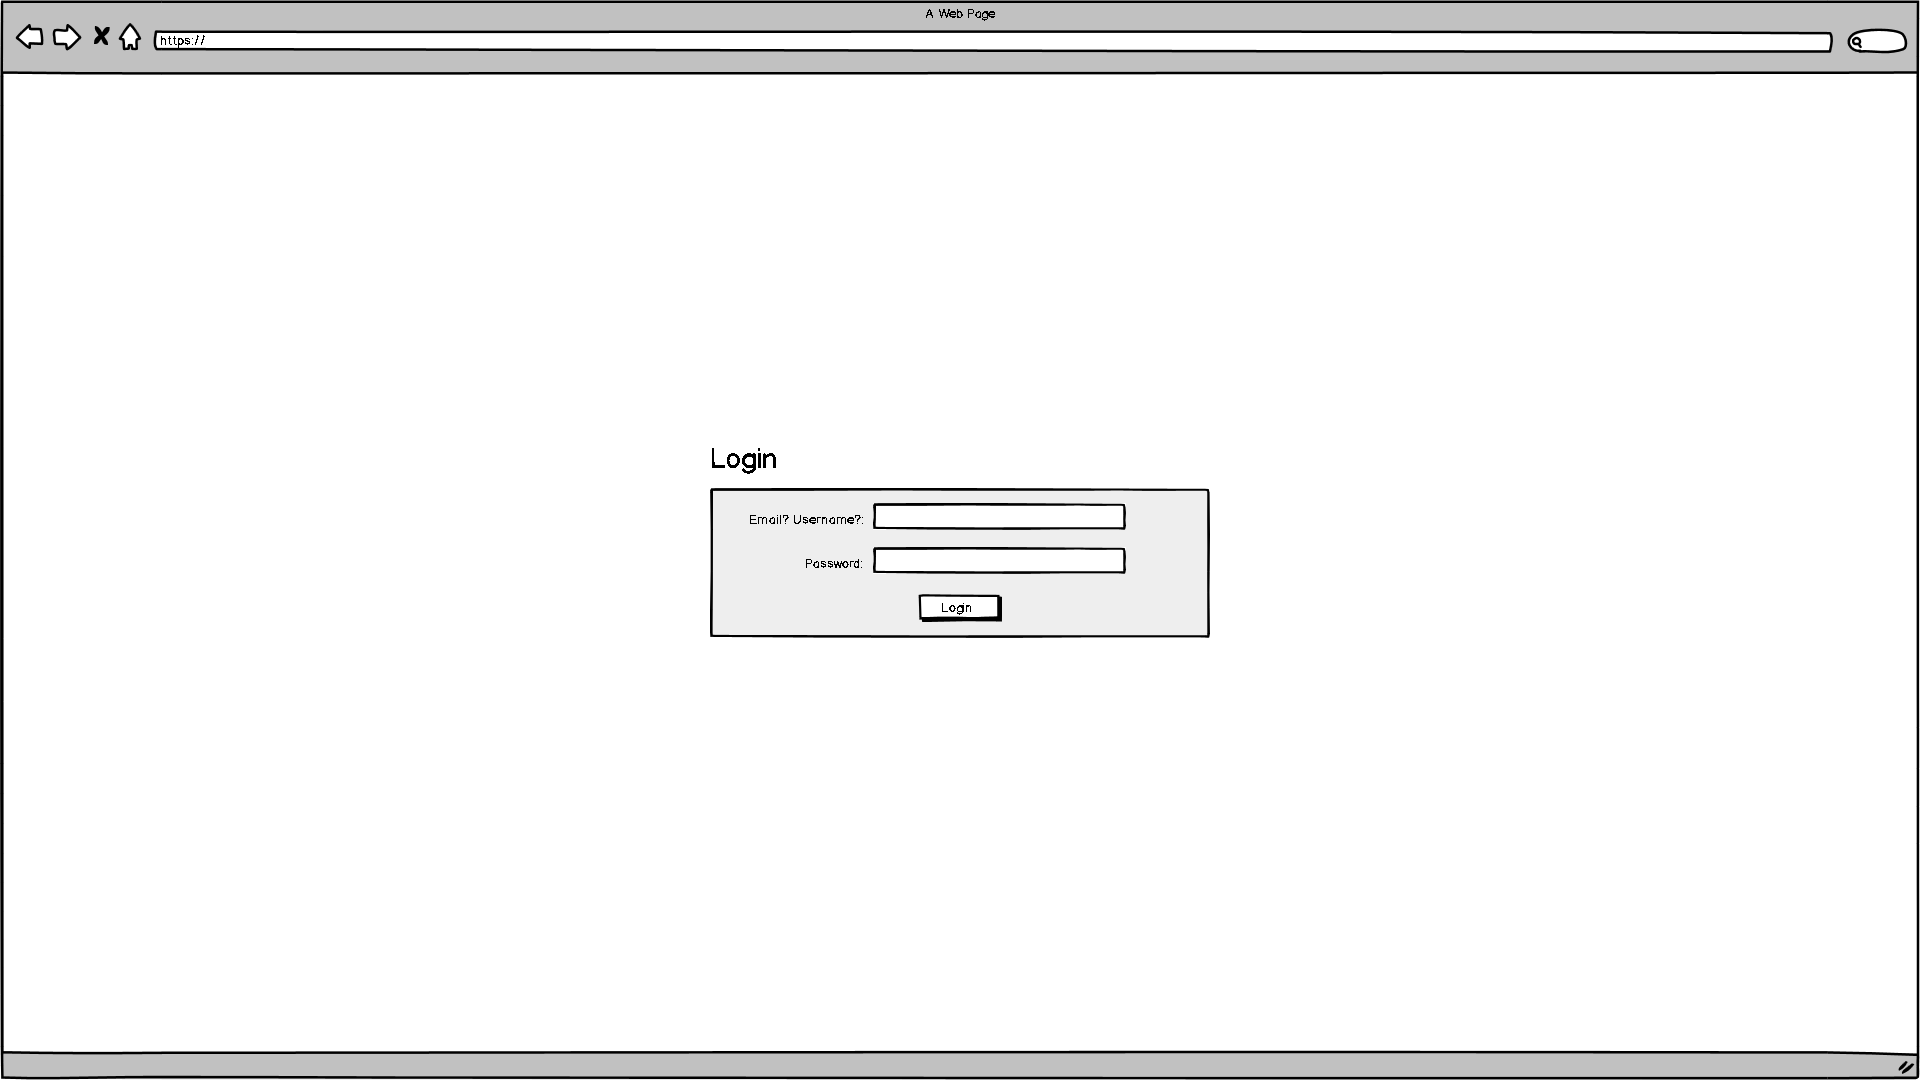
\includegraphics[width=\textwidth]{Images/01MWL.png}
	\caption{The Login Windows shown as the page is first loaded}
	\label{fig:loginWindow}
\end{figure}


\begin{figure}[ht]
	\centering
	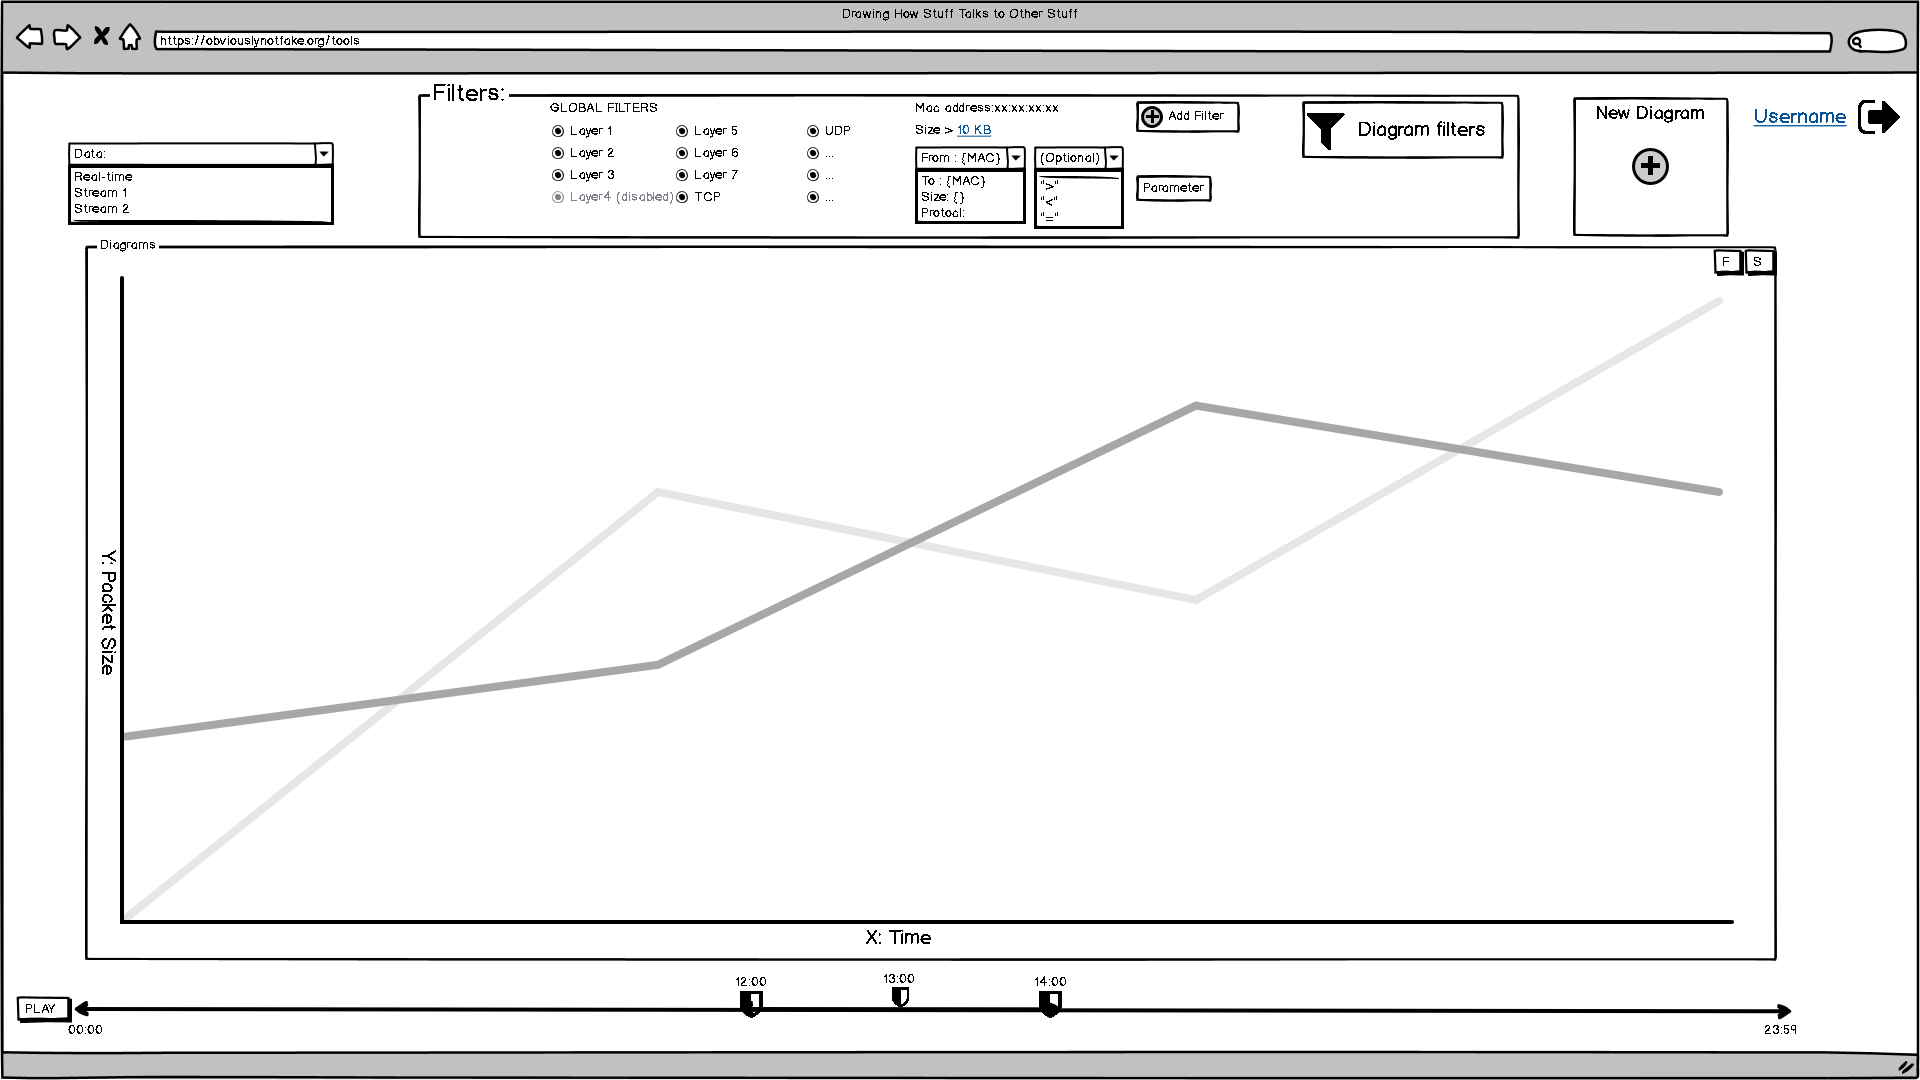
\includegraphics[width=\textwidth]{Images/02MW.png}
	\caption{The Main window the user sees once he logs in}
	\label{fig:mainWindow0}
\end{figure}
\vfill
\clearpage

To discuss in depth this interface it has been divided into subsections labeled in \autoref{fig:mainWindow5}, these are:
\\
\begin{enumerate}
	\item The Data stream drop down menu allows the user to select which stream he is currently listening to. This dropdown menu shows the selected diagram's selected data stream and by default is set to real-time.
	\item Here the user can set filters affecting all diagrams, namely limiting which layers and protocols are currently being shown. To add a new filter a user would click on the add filter button, select which part of the data stream is to be used in the filter, any optional comparators, and set a parameter in the text-box.
	\item This button opens the diagram filter list. This list contains filters specific to each diagram.
	\item By clicking this button the user can create a new diagram. The creation workflow is shown in \autoref{fig:mainWindow1} to \autoref{fig:mainWindow5}.
	\item Here is the currently logged in user, by clicking the button to the right of his name the user can log out.
	\item This is the \gls{diagram container}, inside are all diagrams the user has created with all the set constraints. At most 4 diagrams are shown in the container, and more can be made visible via the slider on the right of the container.
	\item This is a diagram.
	\item By hovering with the mouse over a data point a tooltip is shown with all data associated with this data point.
	\item These buttons control whether a diagram is fullscreen and the diagram settings. By clicking the button labeled F the diagram grows to take on all available space in the container, like shown in \autoref{fig:mainWindow0}.
	      \\
	      Clicking on the button labeled "S" replaces the diagram with the Settings for this diagram like shown in \autoref{fig:mainWindow1}
	\item The play button starts and stops auto scroll along the selected time frame
	\item This is a timeline represented as a slider. It shows on the left and right bottom labels the beginning and end of all data streams.
\\ The labels on top show the currently selected time window and are movable to increasea nd decrease the time window.
\\ The middle shield icon shows the current time while being played, and is also movable to scroll by data manually.

\end{enumerate}


\vfill

\begin{figure}[ht]
	\centering
	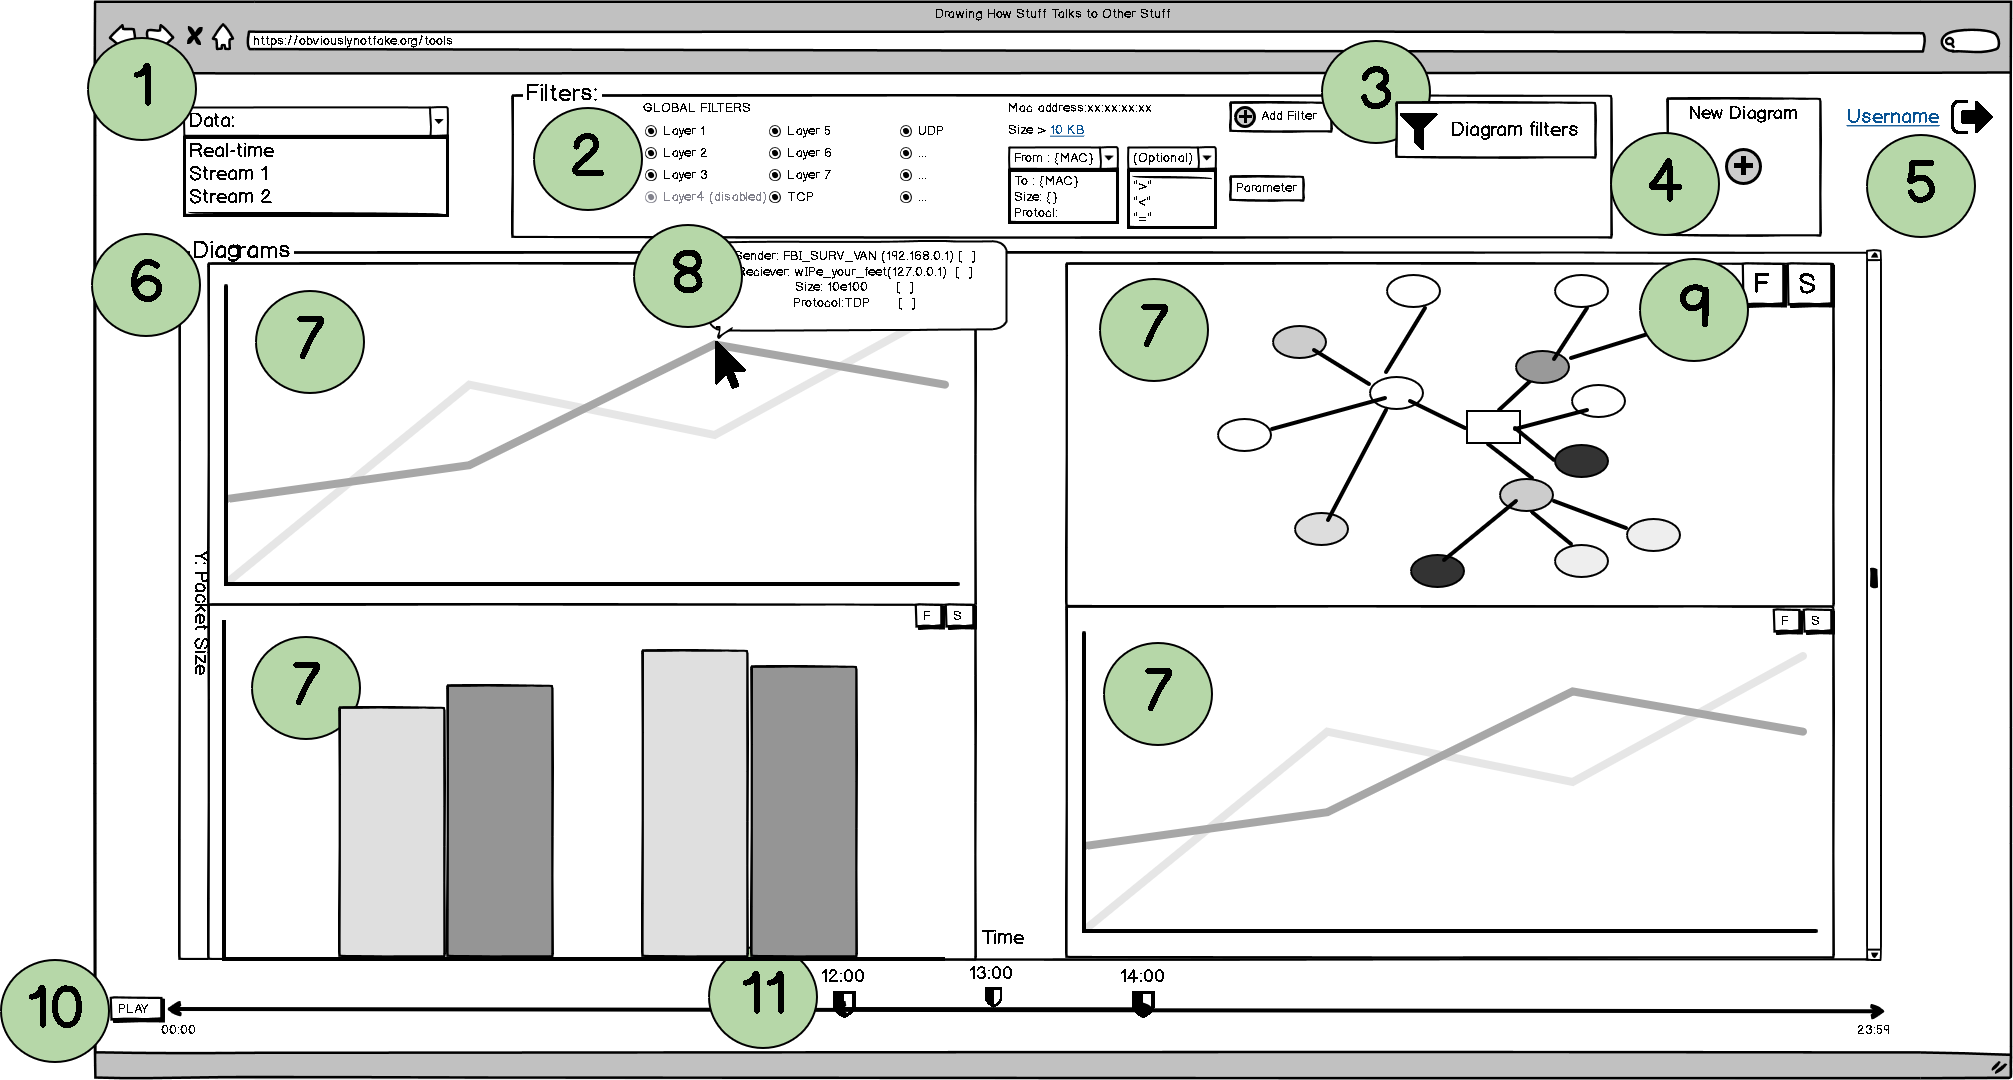
\includegraphics[width=\textwidth]{Images/07MW.png}
	\caption{The GUI divided into relevant sections}
	\label{fig:mainWindow5}
\end{figure}

\vfill
\clearpage

Next we'll take a look at the workflow a user will go through when opening a new diagram.
\\
As referenced above \autoref{fig:mainWindow0} is what the user first sees. When he wants to create a new diagram, by clicking the button labeled new diagram, the Main window is split (shown in \autoref{fig:mainWindow1}) and the new diagram settings are shwon where the new diagram will be.
\\
The user sets here the settings for the new diagram, these are:
\\
\begin{itemize}
	\item{Which data stream it draws its data from}
	\item{Which data is pulled to be represented as the x and y axis}
	\item{Any filters the user wants to apply at the start}
\end{itemize}

Afterwards, the screen looks like \autoref{fig:mainWindow2}, the \gls{diagram container} split in half. By going through this process two more times the diagram container fills up, containing four diagrams total (shown in \autoref{fig:mainWindow3}); at this point the diagrams have their minimum size.
\\
Any diagrams created afterwards are spawned underneath the existing ones and the user can scroll up and down to view all of them (shown in \autoref{fig:mainWindow4}) 



\vfill

\begin{figure}[h]
	\centering
	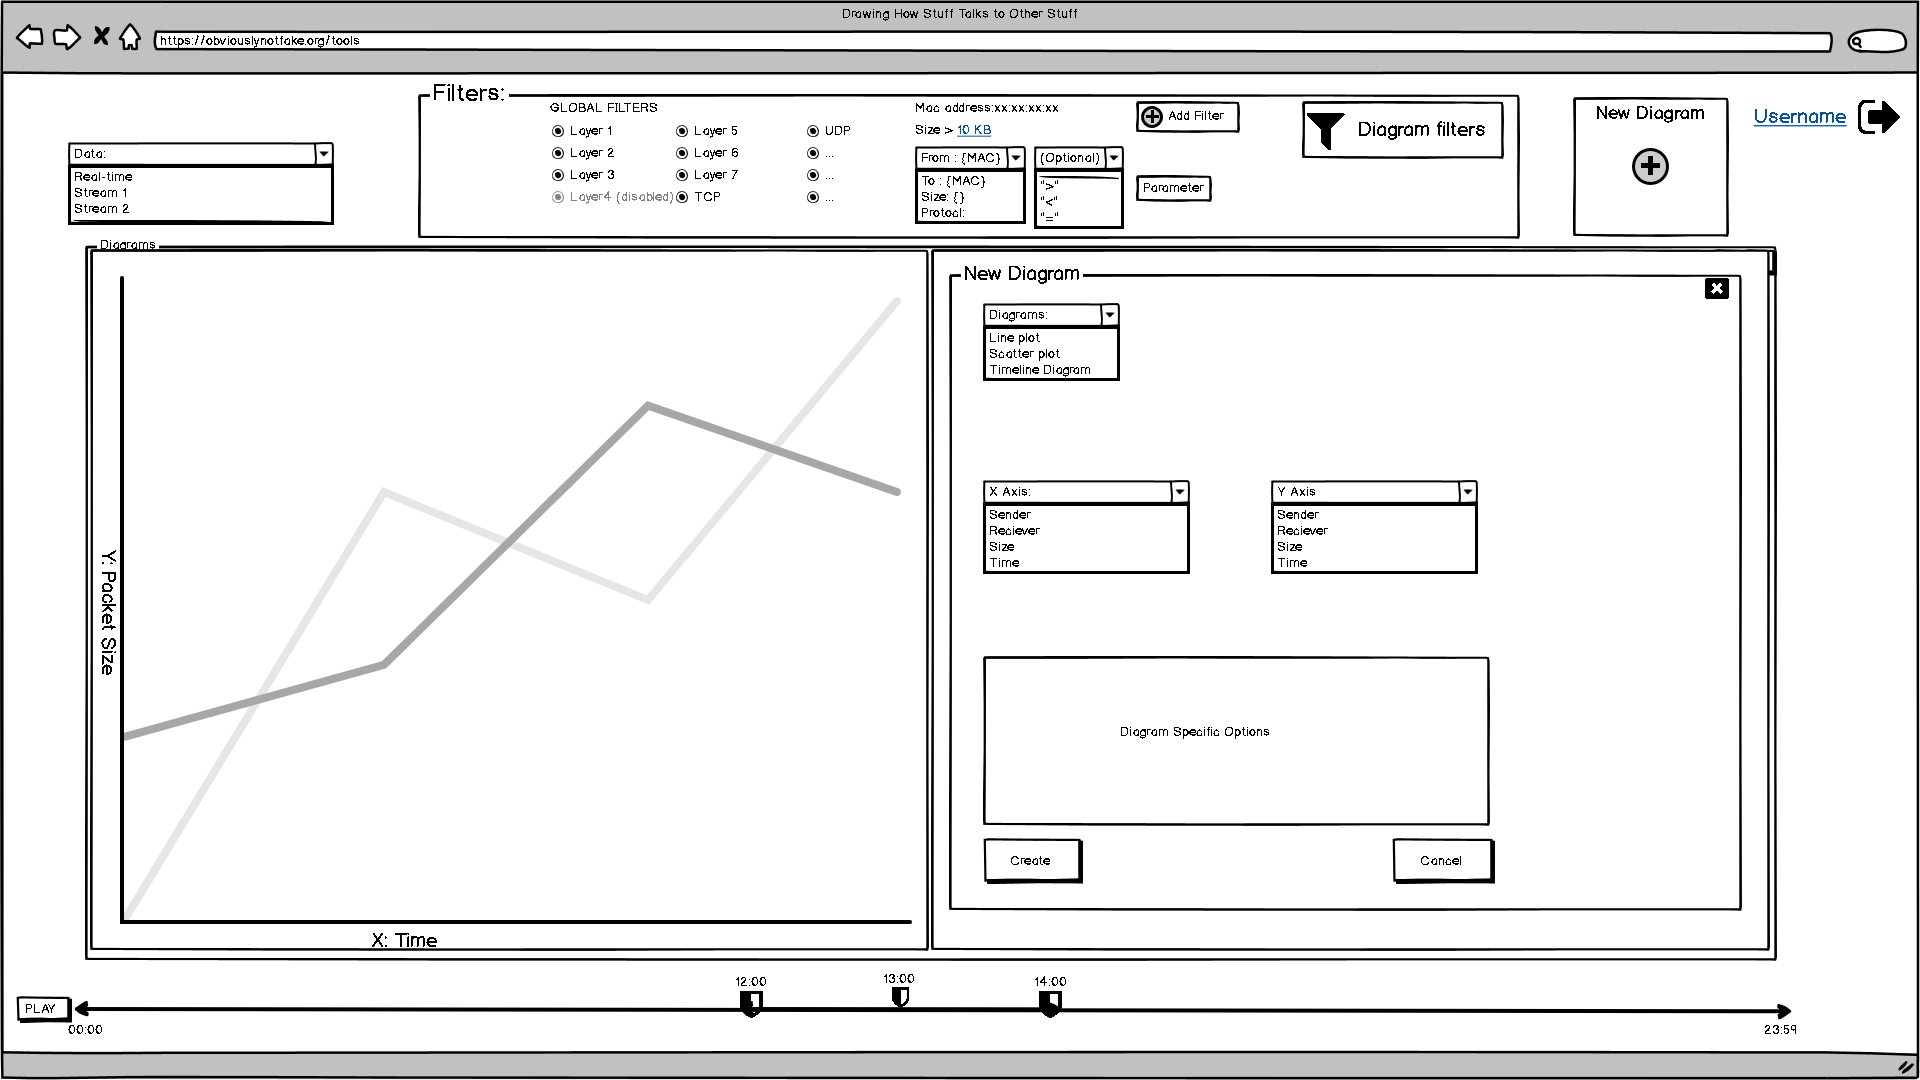
\includegraphics[width=\textwidth]{Images/03MW.png}
	\caption{Main window split in two after user has clicked on the "New diagram" button. New diagram options are set up on the right.}
	\label{fig:mainWindow1}
\end{figure}


\vfill

\begin{figure}[h]
	\centering
	\label{fig:mainWindow2}
	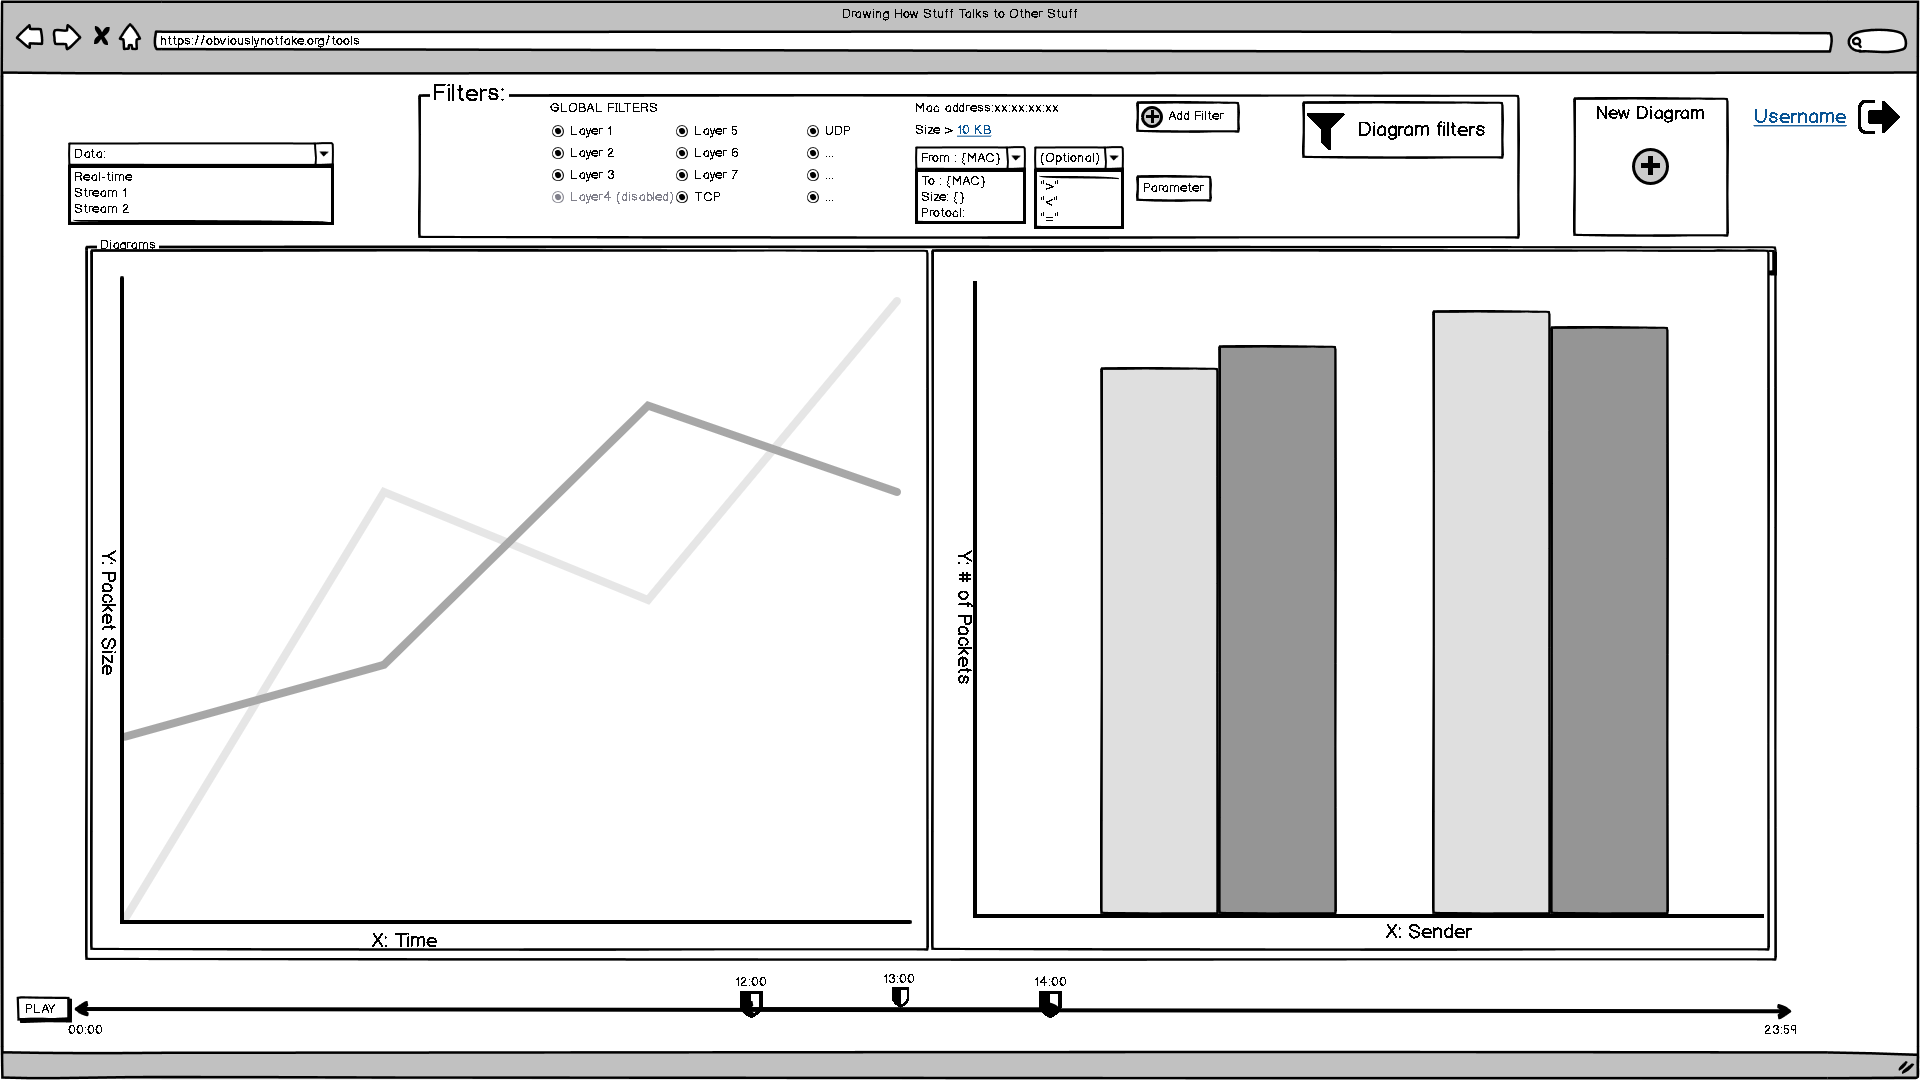
\includegraphics[width=\textwidth]{Images/04MW.png}
	\caption{Main Window with two diagrams side by side.}
	\label{fig:mainWindow2}
\end{figure}



\begin{figure}[h]
	\centering
	\label{fig:mainWindow3}
	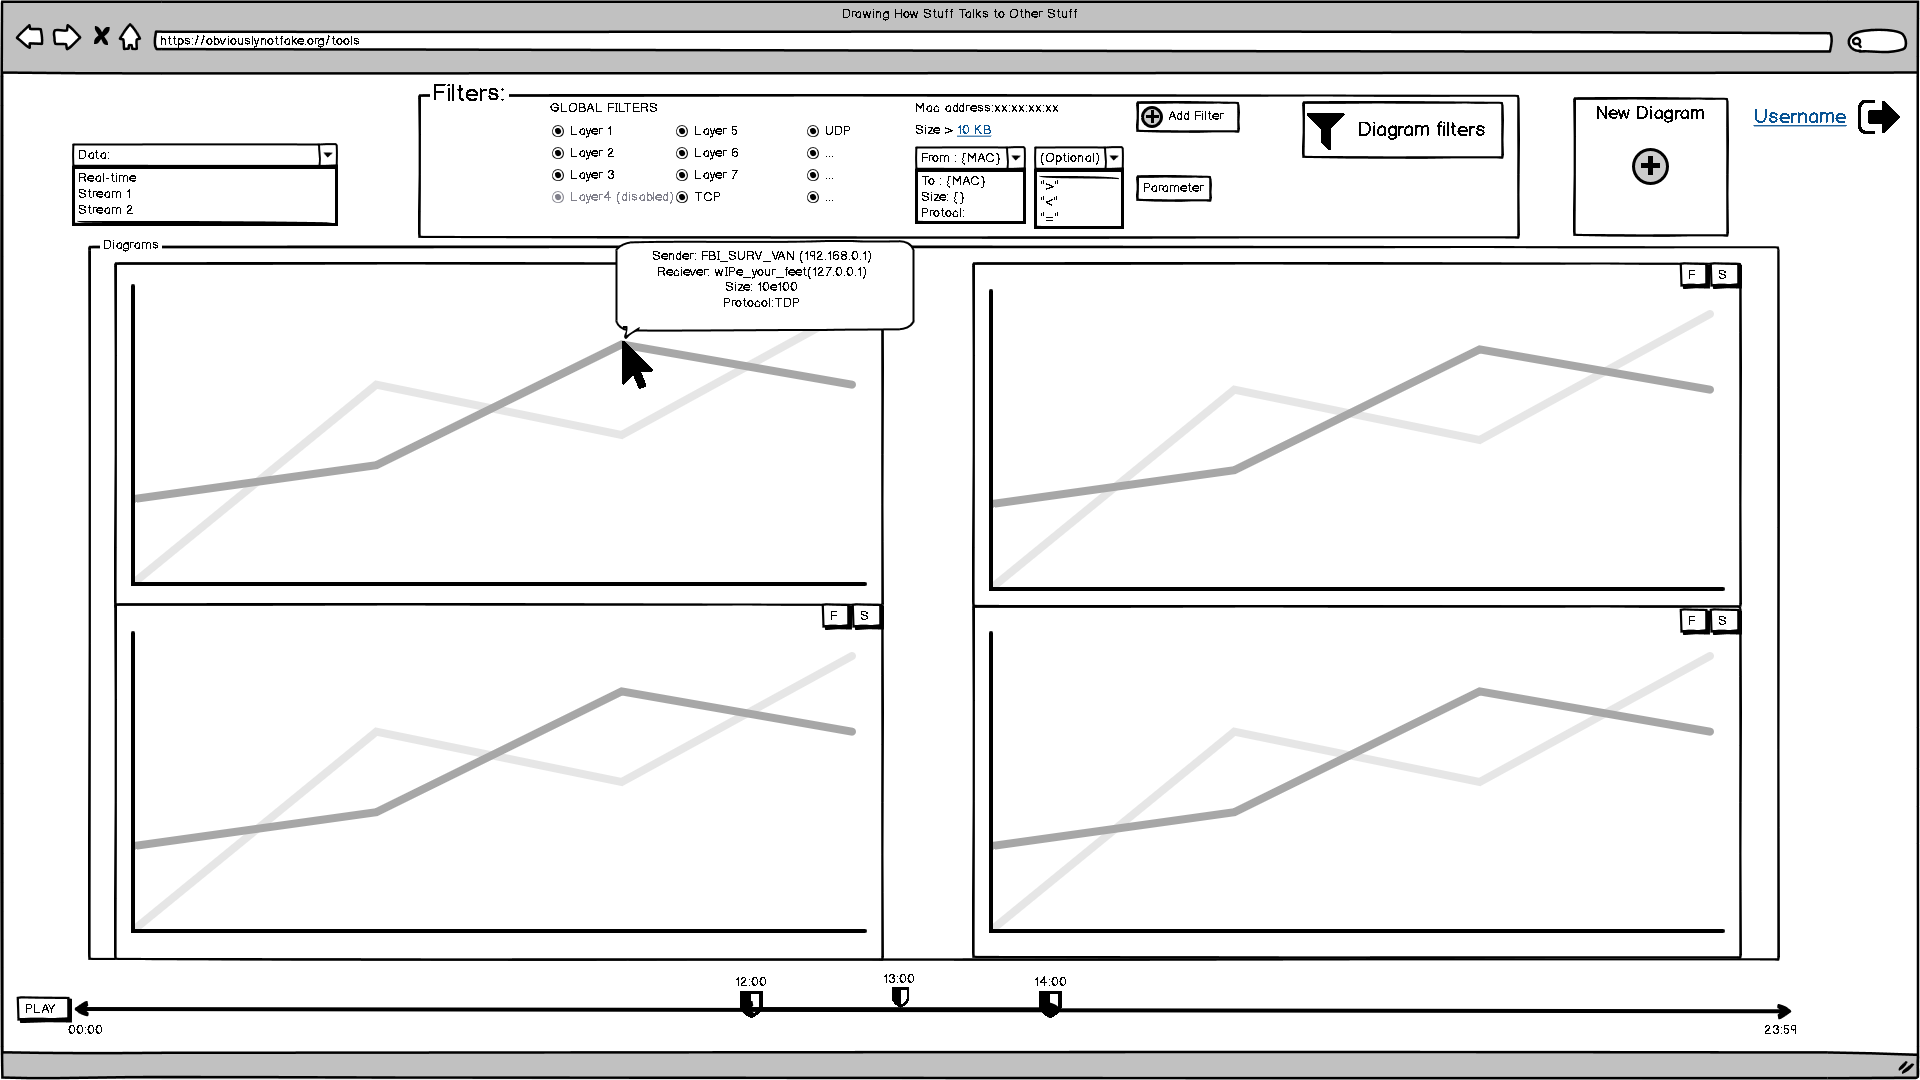
\includegraphics[width=\textwidth]{Images/05MW.png}
	\caption{Main window with four diagrams open}
	\label{fig:mainWindow3}
\end{figure}

\begin{figure}[h]
	\centering
	\label{fig:mainWindow4}
	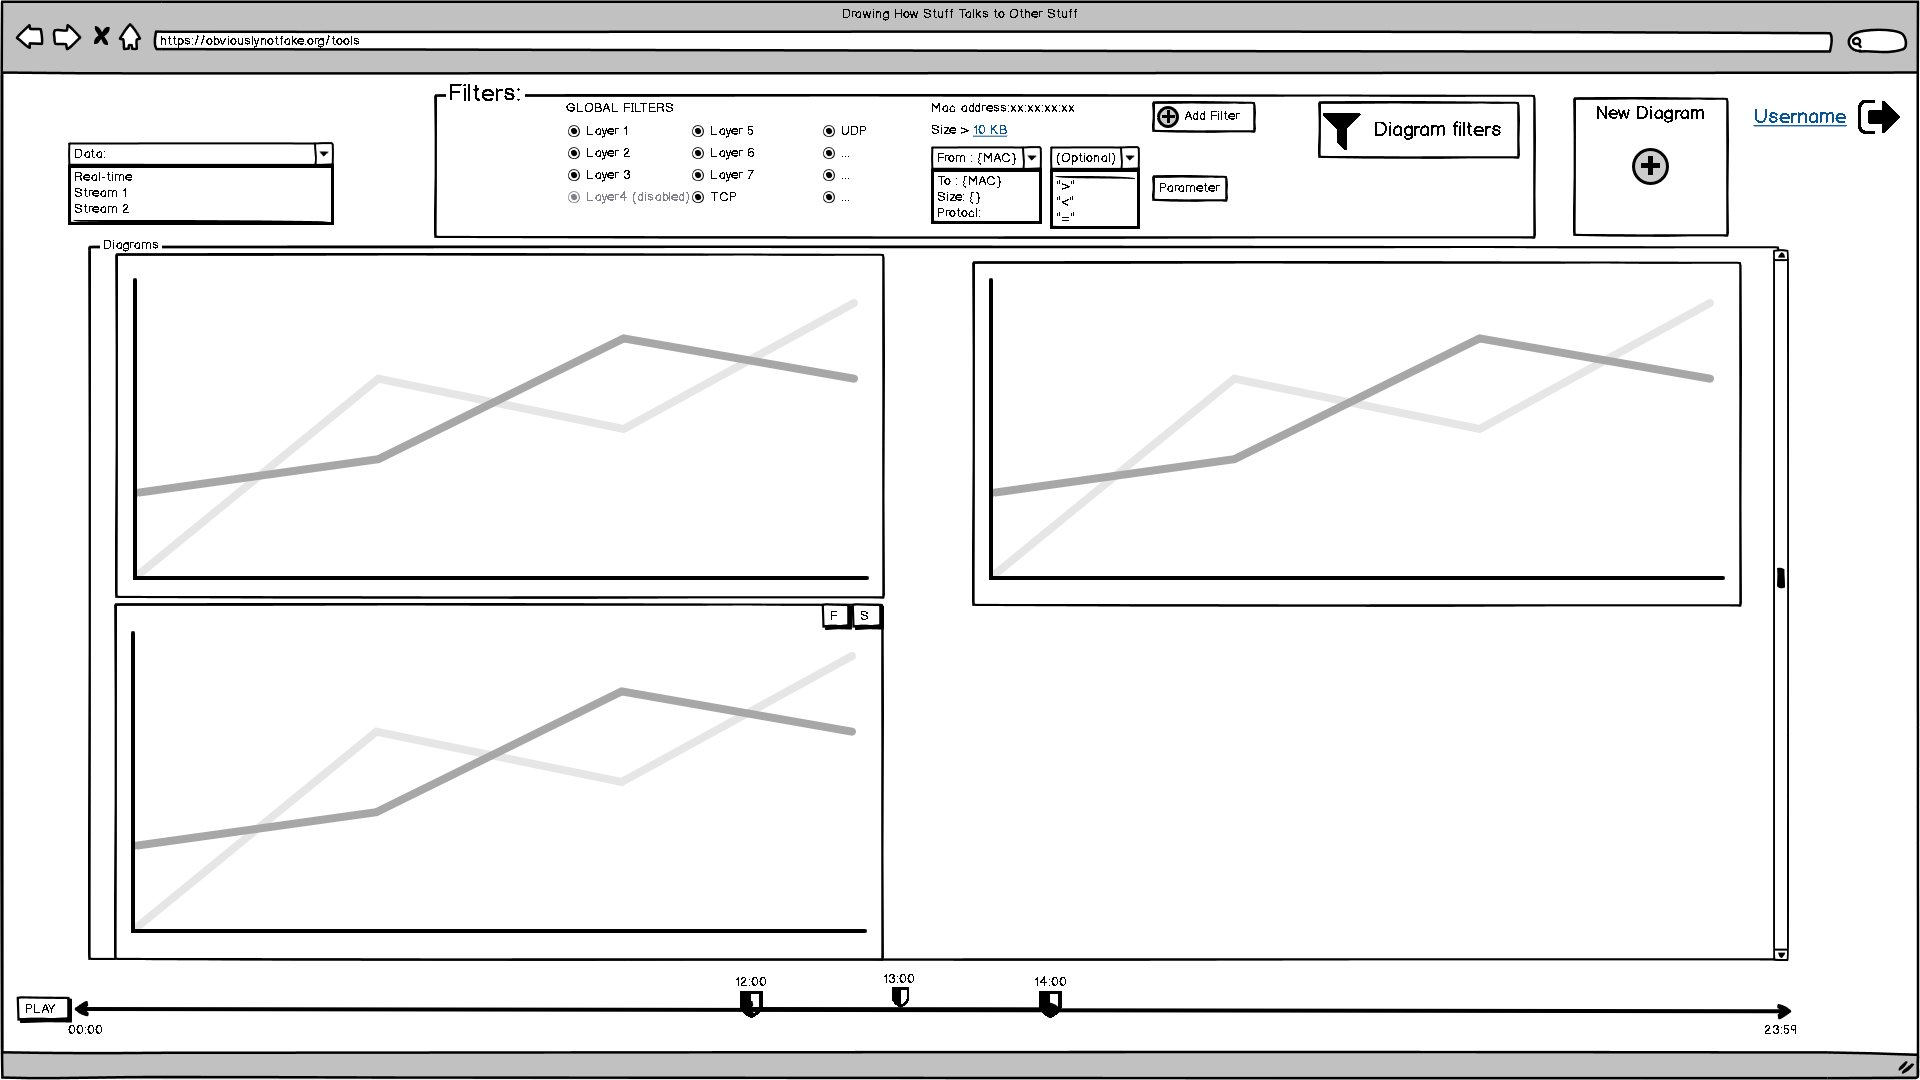
\includegraphics[width=\textwidth]{Images/06MW.png}
	\caption{Main window with more than four diagrams open, more diagrams can be shown using the scroll bar}
	\label{fig:mainWindow4}
\end{figure}

Another activity the user will use frequently is the filtering system.
\\
In the previous section we took a look at the Main window and its different sections. There we described that filters that apply to every diagram are shown at all times shown as item 2. But what about when the user wants to create a filter that only affects one diagram?
\\
For that, the user would click on the Diagram filter (see previous section), an overlay would cover the whole window and a new set of containers, similar to the global filter, would appear, as seen on \autoref{fig:mainWindow6}
\\
On the top we see the global filter list, below it we see the filter list corresponding to the first diagram (diagram numbering is done left to right and top to bottom).
\\
In order to set a new filter that applies to only one diagram the user would open this screen, search for the corresponding diagram number and click on the "add filter button" at which point the button get's moved down to make space for a drop down menu containing all types of data from a data stream. The user selects one, and depending on which one, if appropriate, another drop down menu appears, with contextual relational symbols (i.e. less than (<), equals, etc.) and next to it a text box where the user can input the matching string to which to filter.


\begin{figure}[h]
	\centering
	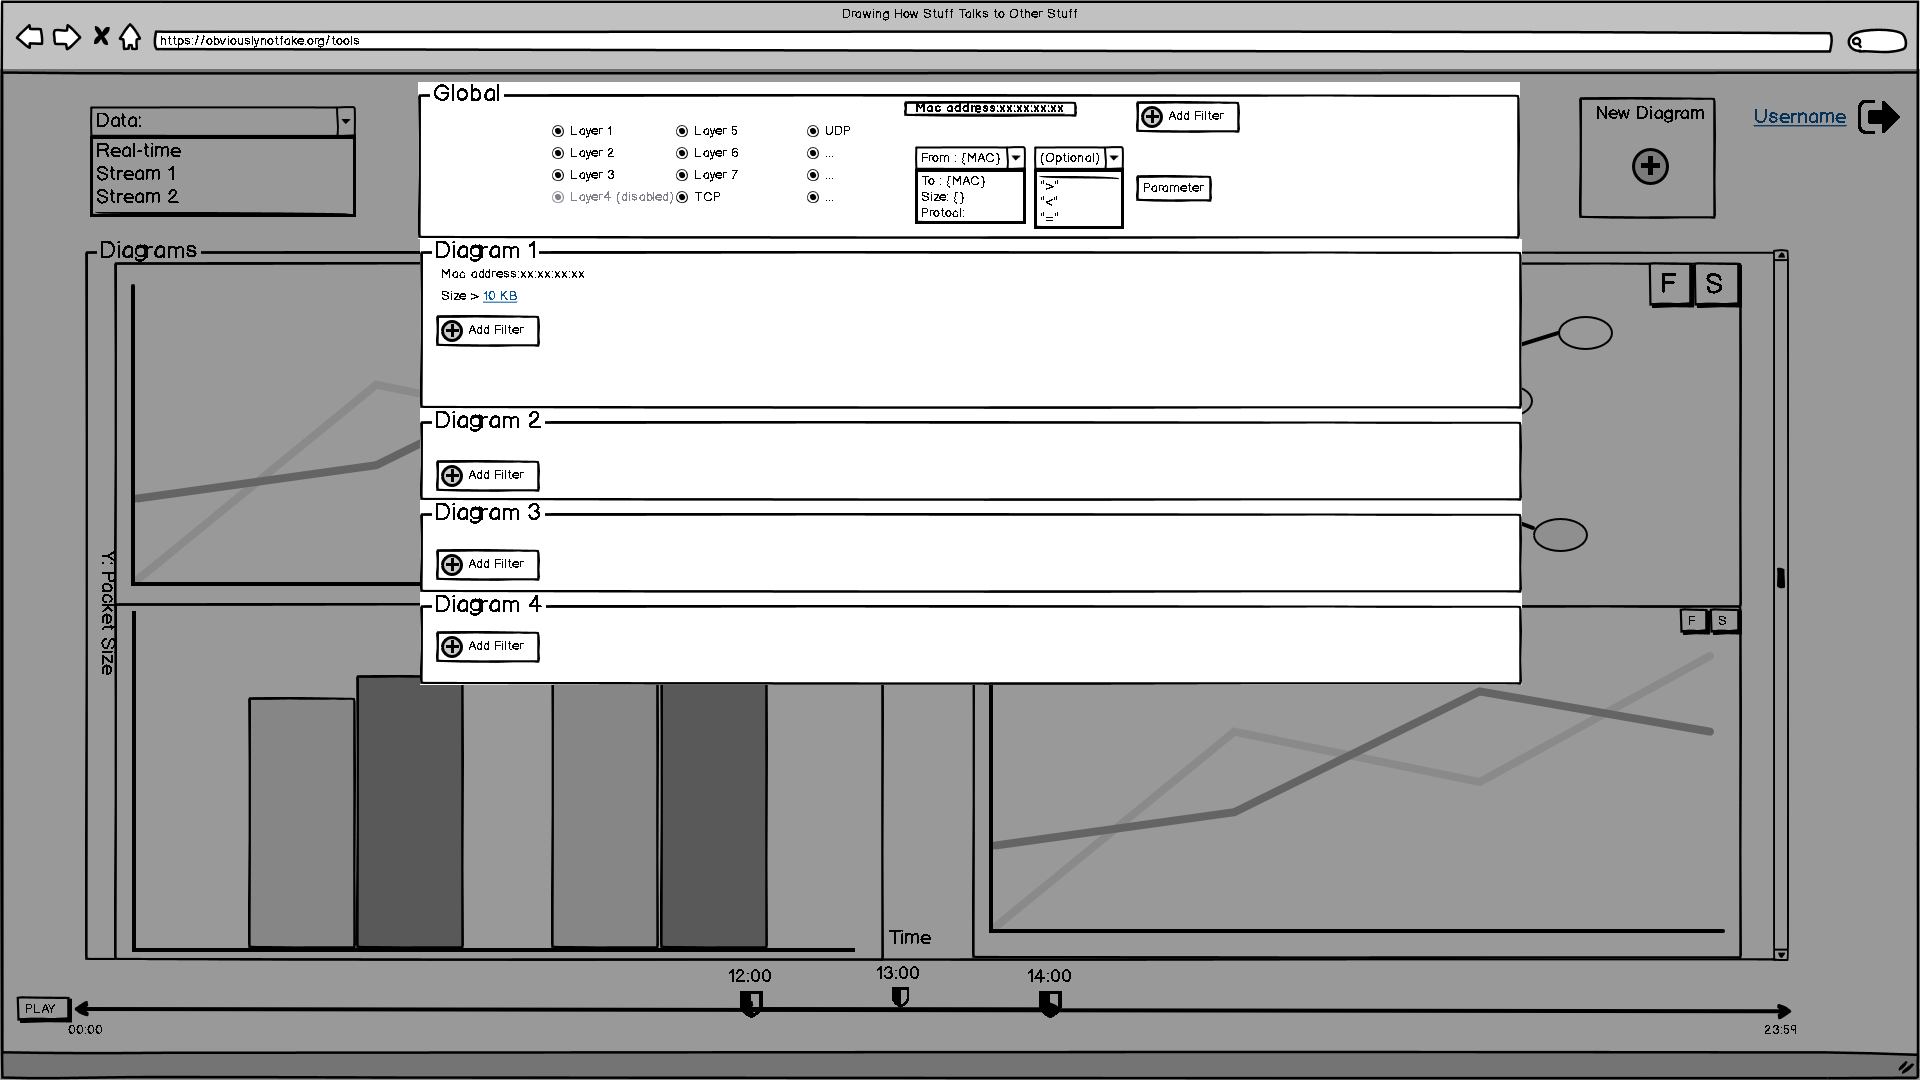
\includegraphics[width=\textwidth]{Images/09MW.png}
	\caption{Main window with more than four diagrams open, more diagrams can be shown using the scroll bar}
	\label{fig:mainWindow6}
\end{figure}
\clearpage

\subsubsection{Diagram types}
Next we'll discuss the four basic diagram types that comprise the minimum scope of this project and their possible use cases.
These are ~\autoref{fig:Diagram types}:

\begin{itemize}
	\item[] \textbf{Line chart}: to easily compare, linearly, two variables from a data stream.
~\autoref{fig:Diagram types}(a)
	\item[]\textbf{Network Diagram}: provides a simple way to visualize the network topology. This diagram also gives the user the ability to inspect the nodes of the network and select data from a data point to be used as a filter in other diagrams (refer to last section for usage example).~\autoref{fig:Diagram types}(b)
	\item[]\textbf{Raster spike diagram}: this is useful to show the transmission window of each packet and it's corresponding partner.~\autoref{fig:Diagram types}(c)
	\item[]\textbf{Scatter plot}: a way to visualize up to 4 dimensions of the data stream.~\autoref{fig:Diagram types}(d)
\end{itemize}

These are examples and since the user has the ability to chose what part of the data stream is used for each axis it does not convey the full ability of these diagrams, that is left to the end user.
\begin{figure*}[!h]
	\centering
	\begin{subfigure}[h]{0.475\textwidth}
		\centering
		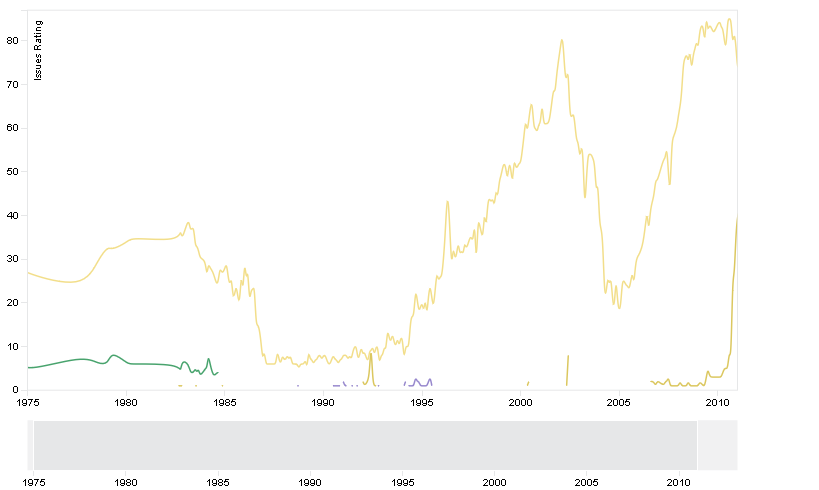
\includegraphics[width=\textwidth]{Images/line_chart.png}
		\caption[Line Chart]%
		{{\small Line Chart}} \cite{Firstarticle}
		\label{fig:Diagram types}
	\end{subfigure}
	\hfill
	\begin{subfigure}[h]{0.475\textwidth}
		\centering
		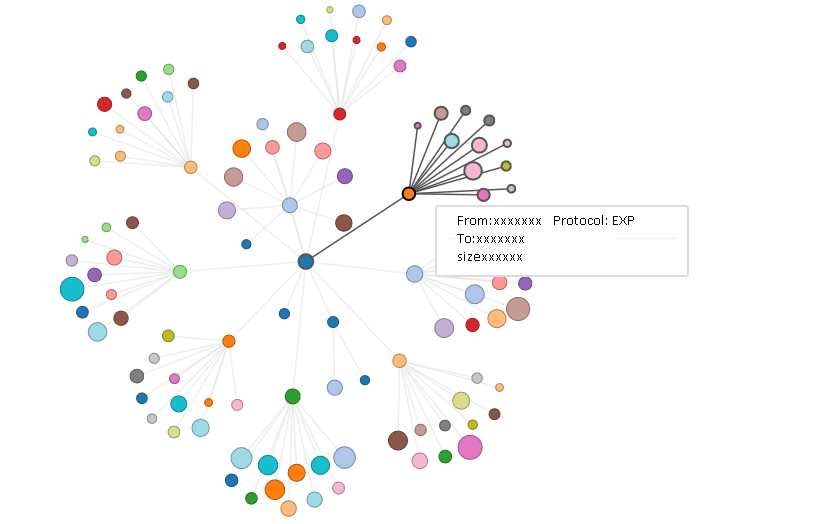
\includegraphics[width=\textwidth]{Images/net_diag.png}
		\caption[]%
		{{\small Net diagram}} \cite{Secondarticle}
		\label{fig:Diagram types}
	\end{subfigure}
	\vskip\baselineskip
	\begin{subfigure}[h]{0.475\textwidth}
		\centering
		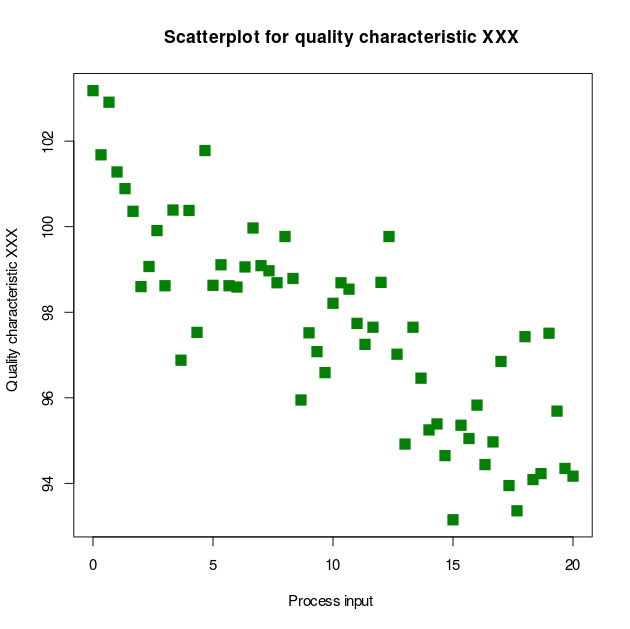
\includegraphics[width=\textwidth]{Images/Scatter_diagram.png}
		\caption[]%
		{{\small Scatterdiagram}} \cite{Thirdarticle}
		\label{fig:Diagram types}
	\end{subfigure}
	\quad
	\begin{subfigure}[h]{0.475\textwidth}
		\centering
		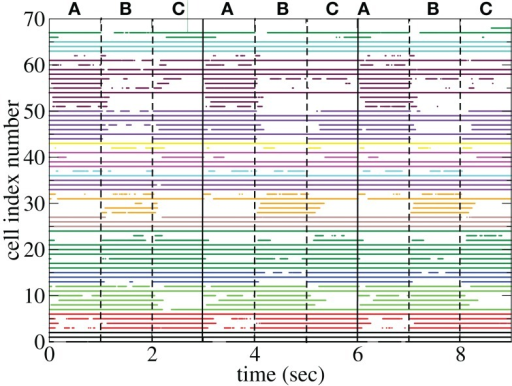
\includegraphics[width=\textwidth]{Images/spike_raster_plot.png}
		\caption[]%
		{{\small Spike raster plot}} \cite{Fourtharticle}
		\label{fig:mean and std of net44}
	\end{subfigure}
	\caption[ Diagram types ]
	{\small Diagram types}
	\label{fig:Diagram types}
\end{figure*}
\vfill
\clearpage
\subsection{Scenarios}

\begin{description}
	\item[S100:] An operator wants to check manually/visually whether network nodes appeared or disappeared over the last day
	      \begin{itemize}
		      \item{the operator opens the web page}
		      \item{the operator selects the database as \gls{data source}}
		      \item{the operator selects a time-line-based \gls{diagram type}}
		      \item{the operator selects node addresses as the data to be displayed}
		      \item{the operator moves to or selects the last 24 hours as the range of data to display}
		      \item{the operator closes the web page}
	      \end{itemize}



	\item[S200:] A security analyst wants to look at the current flow rates between network nodes to see whether they change / there are trends
	      \begin{itemize}
		      \item{the analyst opens the web page}
		      \item{the analyst selects a source of live data}
		      \item{the analyst selects an appropriate visualization type}
		      \item{the analyst selects node addresses as the independent variable}
		      \item{the analyst selects flow rates as the data to be displayed}
	      \end{itemize}



	\item[S300:] A security analyst wants to examine a specific point of data
	      \\
	      Precondition: the analyst has already selected the relevant dataset and visualization type
	      \begin{itemize}
		      \item{the analyst selects a data point}
		      \item{the GUI displays a small pop-up window with all the data of this data point}
		      \item{the analyst right-clicks one of the attibutes in the pop-up window and selects "Display all matching types"}
		      \item{the GUI marks all data points that have the same value in this attribute}
	      \end{itemize}



	\item[S400:] The user wants to look at alarms/notifications (TBD)
	      \begin{itemize}
		      \item{the user opens the web page}
		      \item{the user selects the database as data source}
		      \item{the user selects the data stream from the relevant dissector}
		      \item{the GUI diplays the notifications along a timeline, according oder of occurance}
		      \item{the user right-clicks on the x-axis and selects "use record number"}
		      \item{the GUI diplays the notifications along a timeline adjacently}
	      \end{itemize}



	\item[S500:] The user wants to look at normal data together with alarms/notifications
	      \\
	      Precondition: Scenario S100 apart from closing the web page
	      \begin{itemize}
		      \item{the user selects menu "data", entry "sources"}
		      \item{the GUI displays a list of all known data sources with a checkbox in front of each}
		      \item{the user selects the checkboxes for the data sources they want to examine}
		      \item{the GUI displays data from all these data sources within the currently active visualization}
	      \end{itemize}


\end{description}

\subsection{Use cases}
\begin{figure}[h]
	\centering
	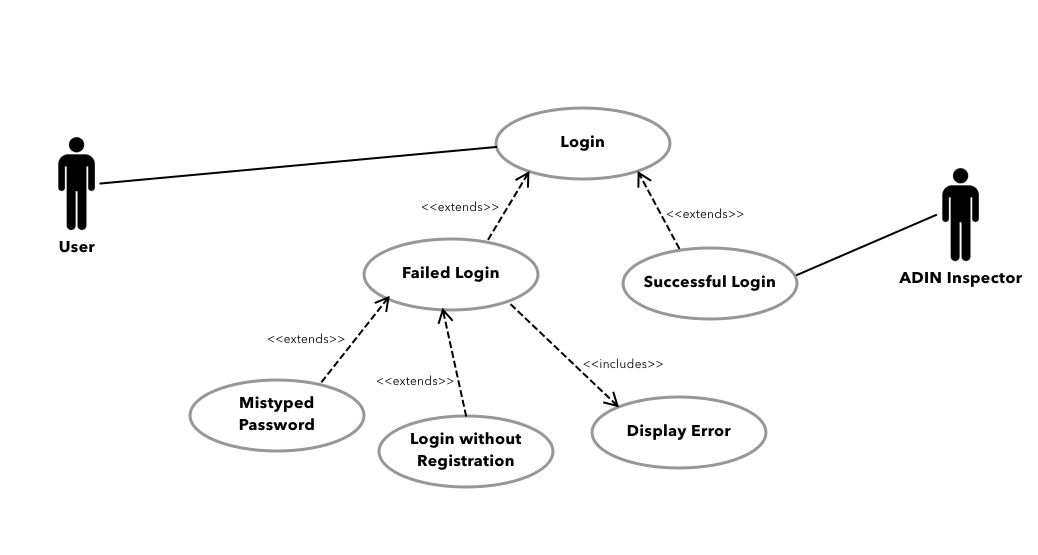
\includegraphics[width=\textwidth]{Images/case_login.PNG}
	\caption{User Login.}
\end{figure}

\begin{description}
	\item[Use Case UC1: Login]
	      \hfill
	      \begin{description}
		      \item[Scope:] ADIN Inspector and hub
		      \item[Level:] user goal
		      \item[Stakeholders and Interests:]
		            \hfill
		            \begin{itemize}
			            \item{User: Wants to login quickly and easily}
			            \item{System administrator: Wants to ensure that only authorized persons access the system. Wants few user support requests.}
			            \item{Manager: Wants protection of data. Wants no obstacle to the user's work.}
		            \end{itemize}
		      \item[Preconditions:] An account for the user has been created.
		      \item[Postconditions:] User is loged in.
		      \item[Main Success Scenario:]
		            \hfill
		            \begin{enumerate}
			            \item{Customer opens the ADIN website in the browser}
			            \item{Customer enters his/her username and password}
			            \item{The ADIN system checks the entered password and loads the access permissions for the user.}
			            \item{The sytem presents the ADIN main screen.}
			            \item{User begins to use the ADIN Inspector.}
		            \end{enumerate}

		      \item[Exception control flow]
		            \hfill
		            \begin{itemize}
			            \item[] Possible at any time: the network connection to the server fails or the server crashes:
			                  \begin{enumerate}
				                  \item{the user reloads the web site which takes him/her to the ADIN login screen}
			                  \end{enumerate}

			            \item[]At step 3: Wrong username or password:
			                  \begin{enumerate}
				                  \item{System produces an error message and stays on the login screen.}
			                  \end{enumerate}

		            \end{itemize}
	      \end{description}

	      \begin{figure}[h]
		      \centering
		      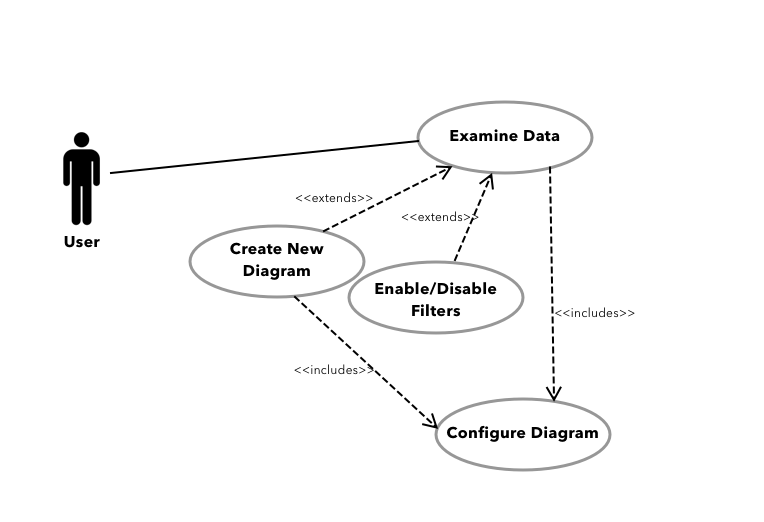
\includegraphics[width=\textwidth]{Images/case_examine_data.png}
		      \caption{Examine Data.}
	      \end{figure}
\end{description}


\subsubsection{Interactivity}

Visual analytics methods combine interactive visualisations with automated analysis
techniques. This allows the user to decide e.g. which part
of the data he or she wants to explore in more detail.

A basic principle for visual data exploration was introduced by Shneiderman (1997) by what he called the “The Visual Information Seeking Mantra:

Overview first, zoom and filter, then details-on-demand”.
This lets the data analyst define to a certain level what he or she wants
to analyze and visualise.

Similar to this, Bertin (1983) specified three “levels of reading,”:
The elementary level (allowing the analyst to look at the information about a
single data record), the intermediate level (showing summarised information about a group of data records), and the global level (providing an overview of all data elements).

\subsection{Object Modelling}

The diagram in \autoref{fig:adin-sys} shows a high-level view of the components of the ADIN-Inspector. The PSE group will develop the visualization component that runs in the web browser and a server side component called hub. The hub interfaces with the data sources and also implements the access control.

\begin{center}
	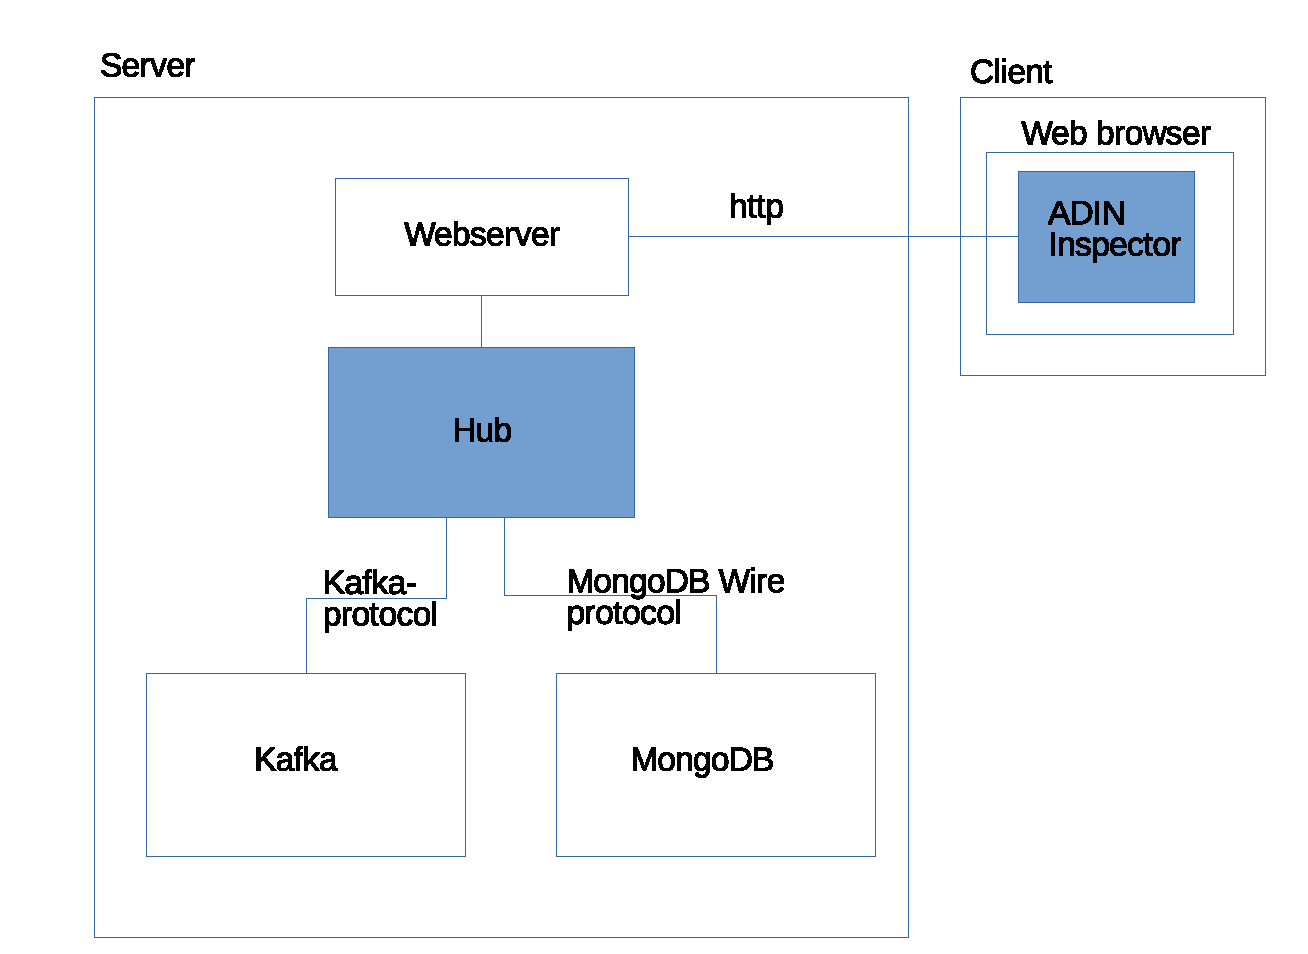
\includegraphics[scale=0.8]{Images/adin-sys1d.eps}
	\captionof{figure}{General system layout. Components to be developed by the PSE group are marked blue.}
	\label{fig:adin-sys}
\end{center}


\subsection{Dynamic Modelling}

The sequence diagram in \autoref{fig:adin-login-seq} shows the actions of the Hub component during login.

\begin{center}
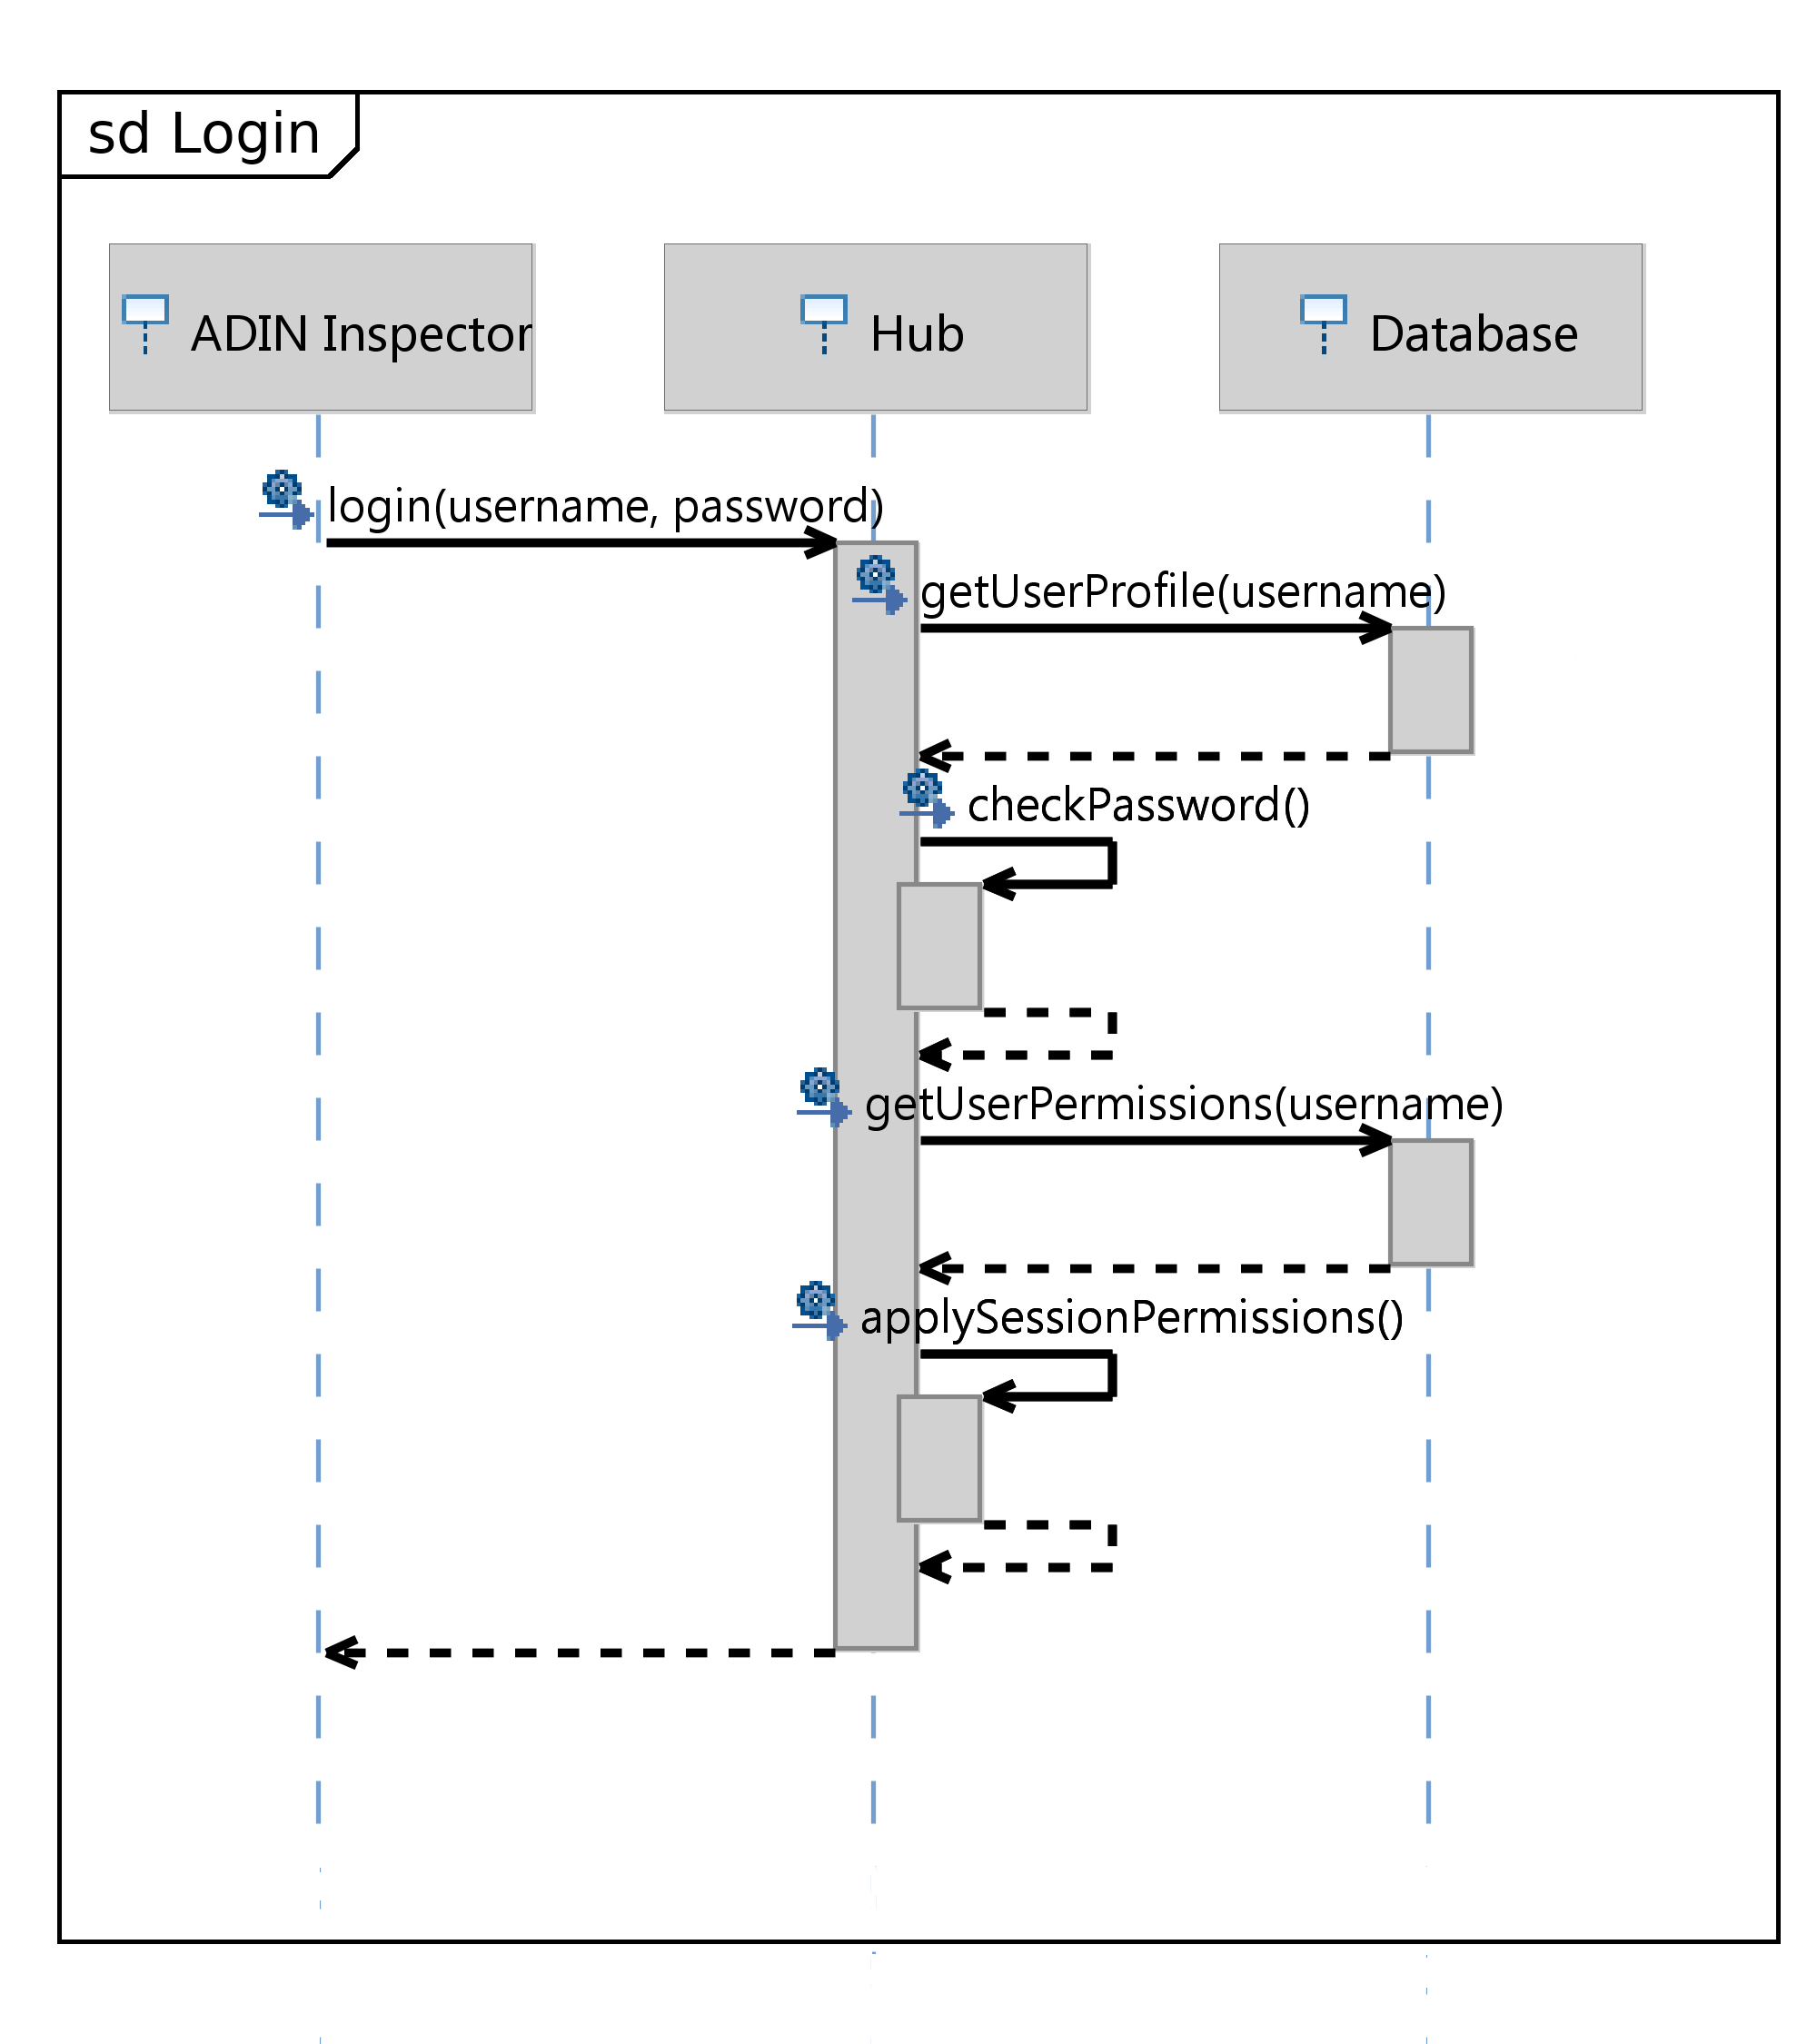
\includegraphics[width=0.8\textwidth]{Images/adin-login-seq.png}
\captionof{figure}{The activity of the Hub during login.}
\label{fig:adin-login-seq}
\end{center}

\section{Glossary}
\printglossary[title=,toctitle=]


%% |   Bibliography   |
%% --------------------

%% Add entry to the table of contents for the bibliography
\printbibliography[heading=bibintoc]

\chapter{Design}\label{sec:design}
\section{Front-End}
This subsection describes the front-end of the ADIN INSPECTOR - the UI elements the GUI consists of, and how states are handled. A series of final UI design mockups are presented under UI Design Mockups subsection, whereas an overview of the GUI classes can be seen in \autoref{fig:gui_overview}.\\

The GUI elements are implemented in \href{https://reactjs.org/}{\color{blue}{React}} and \href{https://material-ui.com/}{\color{blue}{Material UI}}, whereas the internal logic and application state management are written with \href{https://mobx.js.org/}{\color{blue}{MobX}}.

\subsection{UI Design Mockups}

An early stage interactive demo is available at \url{https://adin-frontend.netlify.com}.\\



\begin{figure}[hp]
	\begin{adjustbox}
		{addcode={\begin{minipage}{\width}}
						{\caption{%
							Login screen
						}
						\label{fig:mockup_login}
					\end{minipage}}
			,center}
		\fbox{
\includegraphics[max size={\textwidth}{0.4\textheight}]{images_design/loginNew.PNG}}
	\end{adjustbox}
\end{figure}

\begin{figure}[h!]
	\begin{adjustbox}
		{addcode={\begin{minipage}{\width}}
						{\caption{%
							Initial empty screen
						}
						\label{fig:mockup_empty}
					\end{minipage}}
			,center}
		\fbox{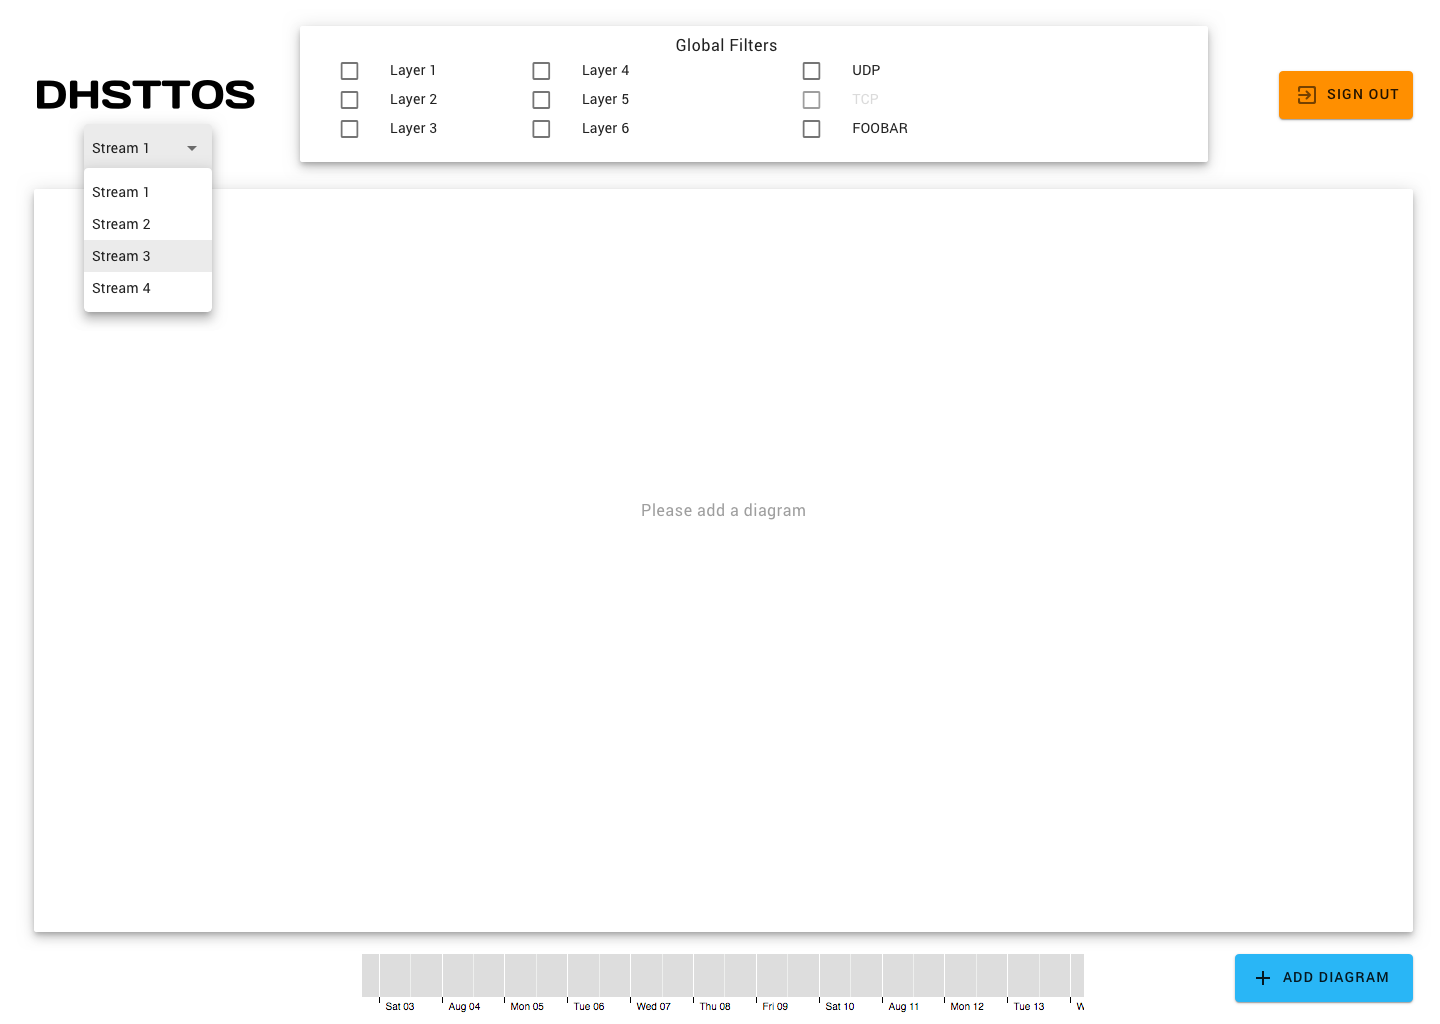
\includegraphics[max size={\textwidth}{0.4\textheight}]{images_design/ui_design/Main/0.png}}
	\end{adjustbox}
\end{figure}

\begin{figure}[h!]
	\begin{adjustbox}
		{addcode={\begin{minipage}{\width}}
						{\caption{%
							Adding first diagram
						}
						\label{fig:mockup_config}
					\end{minipage}}
			,center}
		\fbox{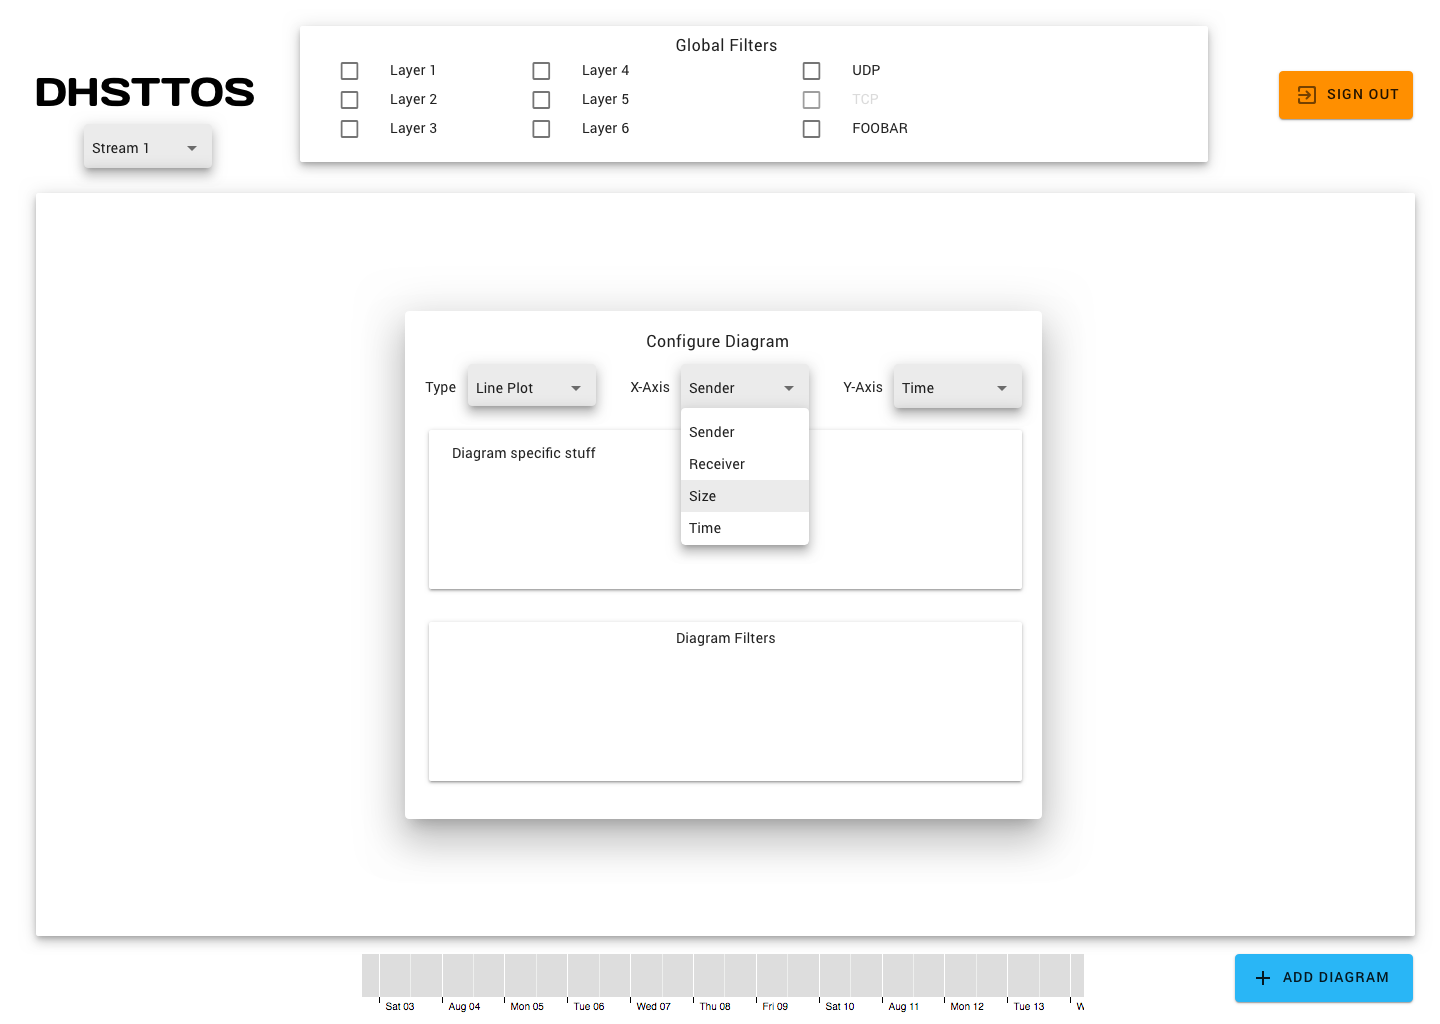
\includegraphics[max size={\textwidth}{0.4\textheight}]{images_design/ui_design/Main/1.png}}
	\end{adjustbox}
\end{figure}

\begin{figure}[h!]
	\begin{adjustbox}
		{addcode={\begin{minipage}{\width}}
						{\caption{%
							Displaying a single diagram
						}
						\label{fig:mockup_single_diagram}
					\end{minipage}}
			,center}
		\fbox{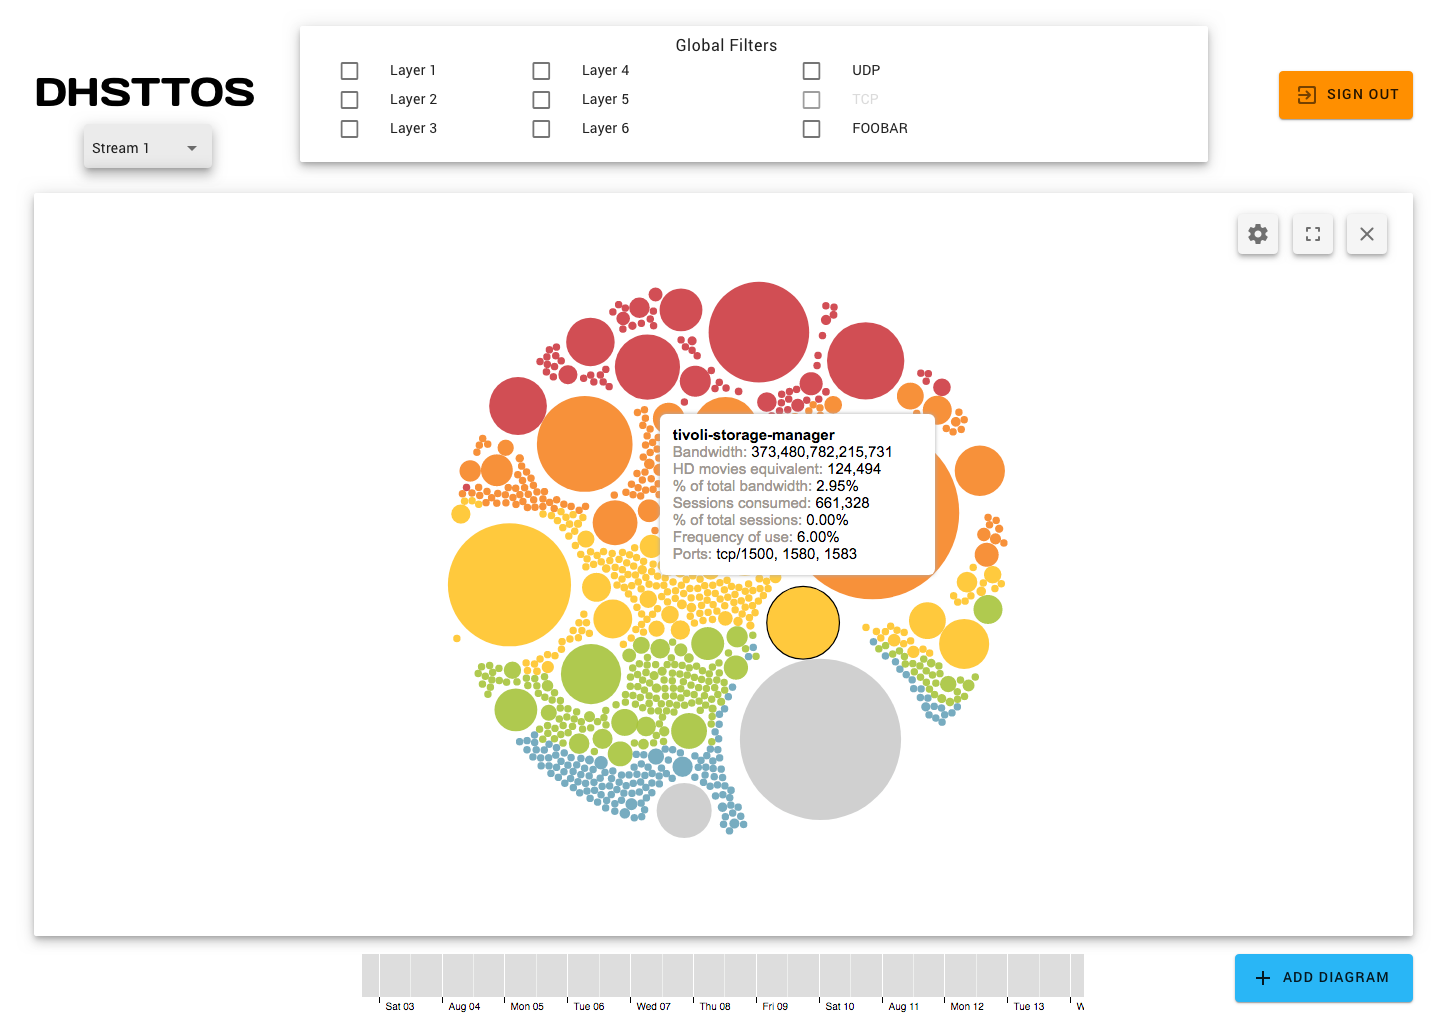
\includegraphics[max size={\textwidth}{0.4\textheight}]{images_design/ui_design/Main/2.png}}
	\end{adjustbox}
\end{figure}

\begin{figure}[h!]
	\begin{adjustbox}
		{addcode={\begin{minipage}{\width}}
						{\caption{%
							Adding new or configuring existing diagram
						}
						\label{fig:mockup_add_diagram_config}
					\end{minipage}}
			,center}
		\fbox{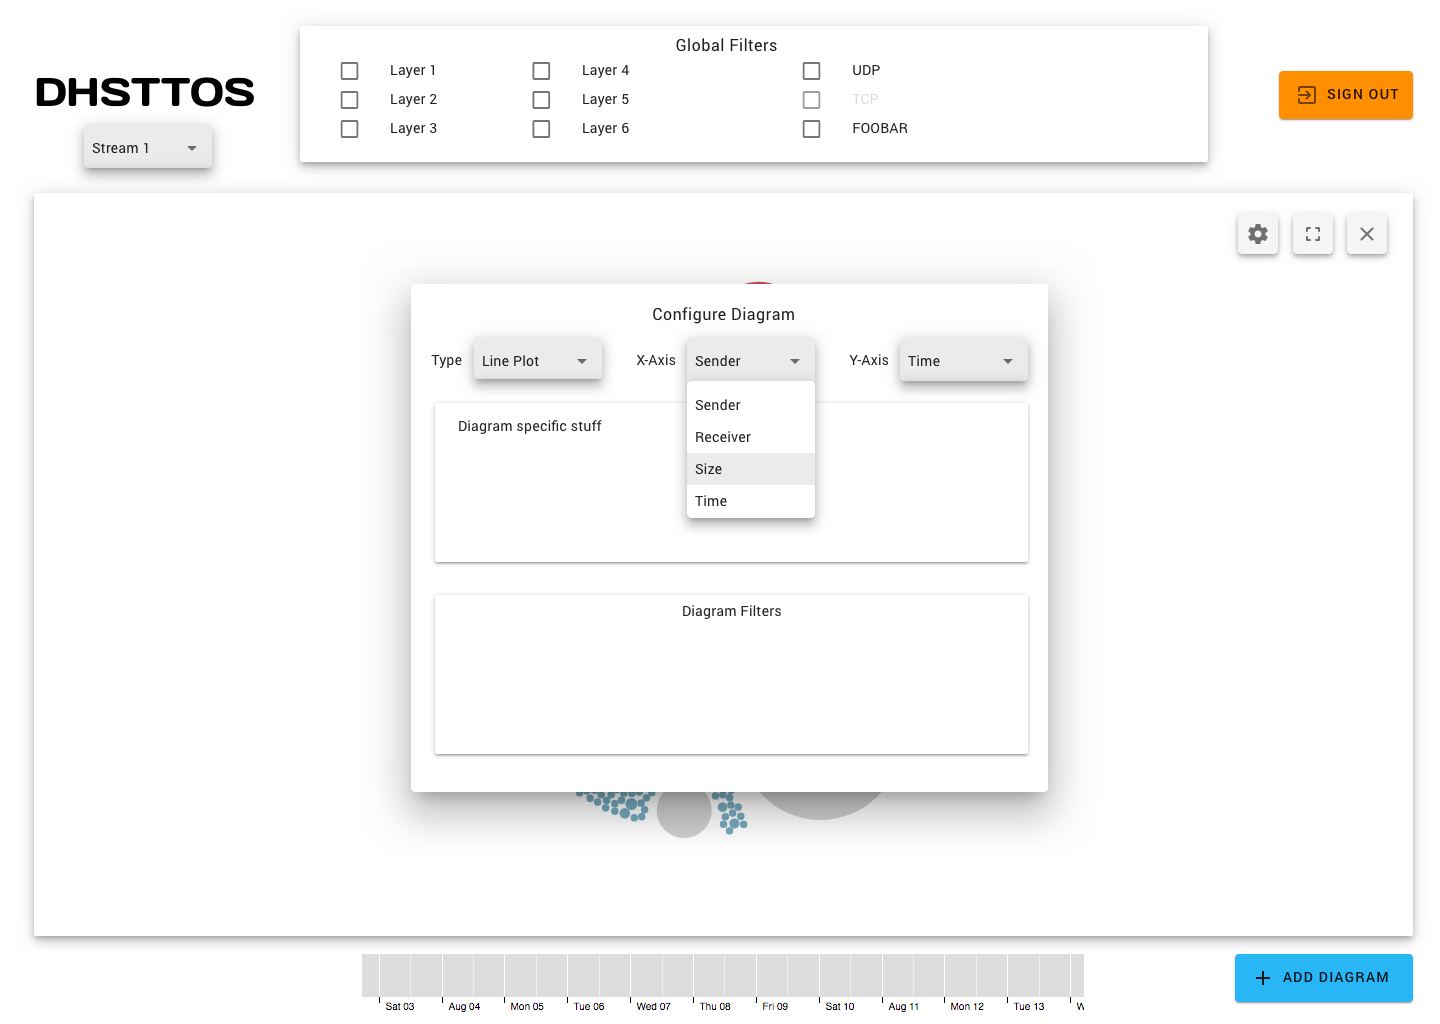
\includegraphics[max size={\textwidth}{0.4\textheight}]{images_design/ui_design/Main/3.png}}
	\end{adjustbox}
\end{figure}

\begin{figure}[h!]
	\begin{adjustbox}
		{addcode={\begin{minipage}{\width}}
						{\caption{%
							Displaying two diagrams
						}
						\label{fig:mockup_two_diagrams}
					\end{minipage}}
			,center}
		\fbox{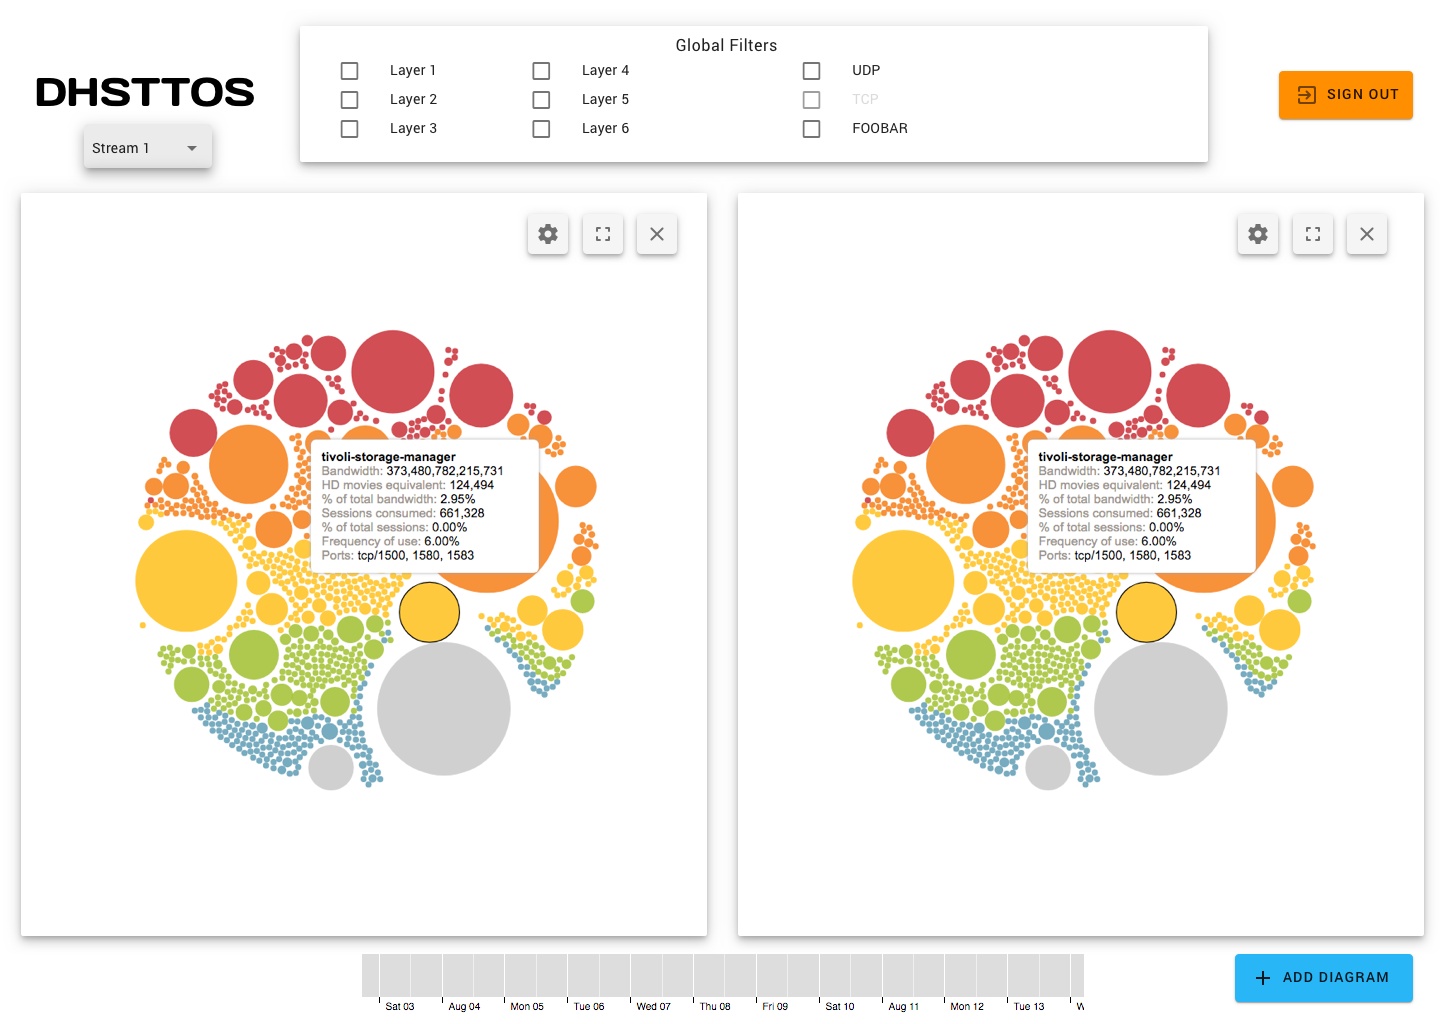
\includegraphics[max size={\textwidth}{0.4\textheight}]{images_design/ui_design/Main/4.png}}
	\end{adjustbox}
\end{figure}

\begin{figure}[h!]
	\begin{adjustbox}
		{addcode={\begin{minipage}{\width}}
						{\caption{%
							Adding additional or configuring existing diagram
						}
						\label{fig:mockup_add_more_diagram_config}
					\end{minipage}}
			,center}
		\fbox{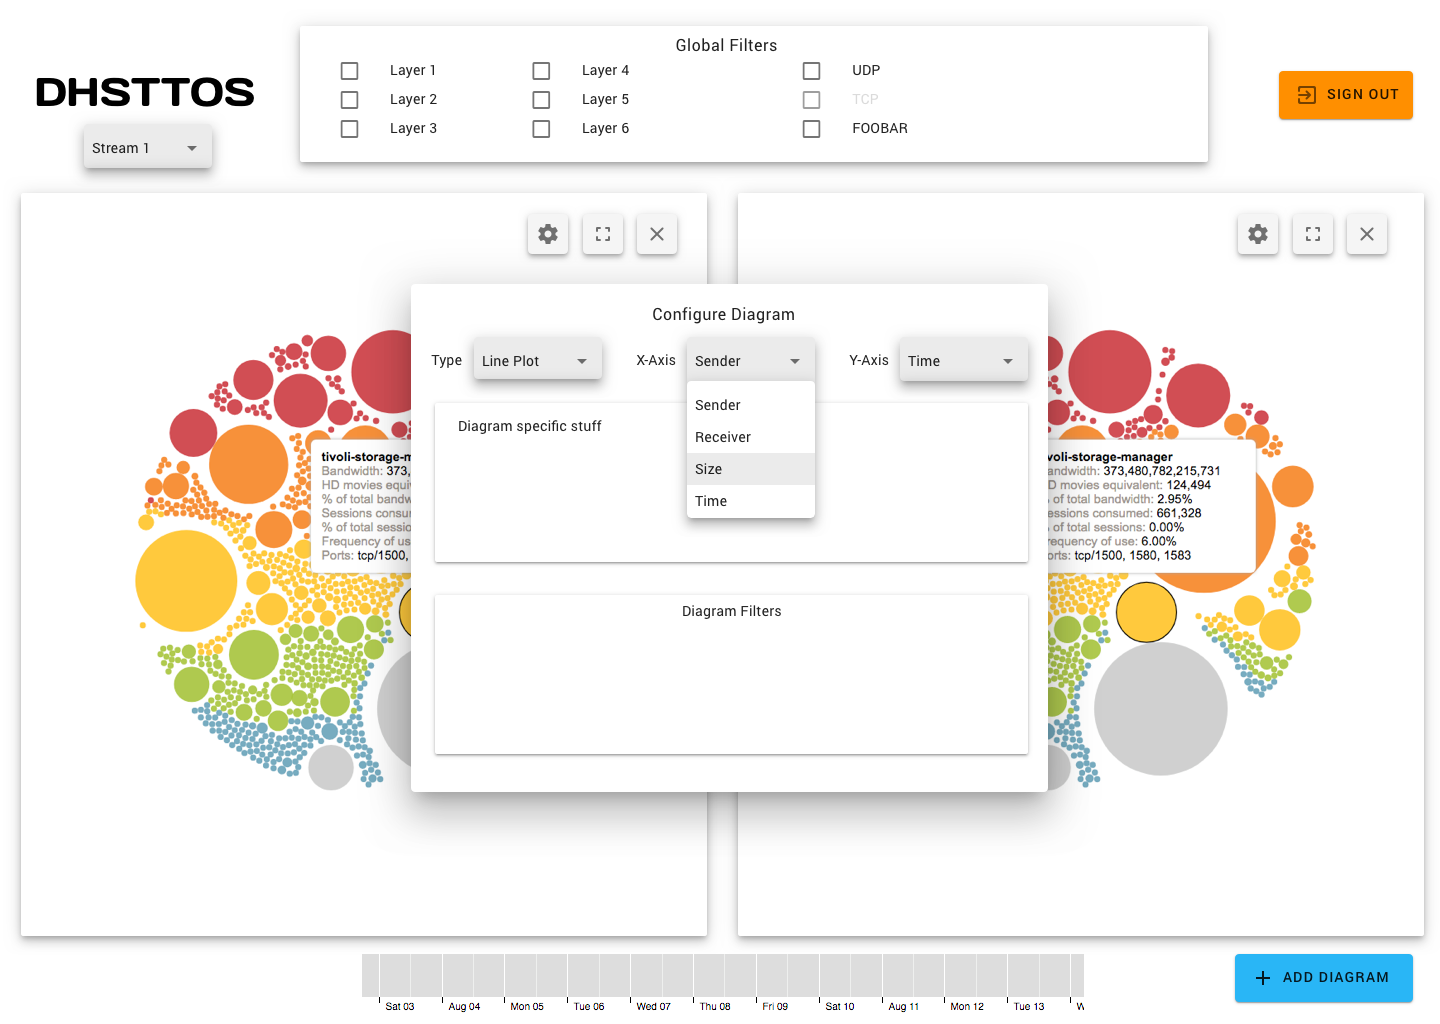
\includegraphics[max size={\textwidth}{0.4\textheight}]{images_design/ui_design/Main/5.png}}
	\end{adjustbox}
\end{figure}

\clearpage

\subsection{Class Diagrams}
\begin{figure}[h!]
	\begin{adjustbox}
		{addcode={\begin{minipage}{\width}}
						{\caption{%
							This diagram shows an overview of GUI elements and their relationships inside the main application, when the user has successfully logged in.
						}
						\label{fig:gui_overview}
					\end{minipage}}
			,rotate=90,center}
		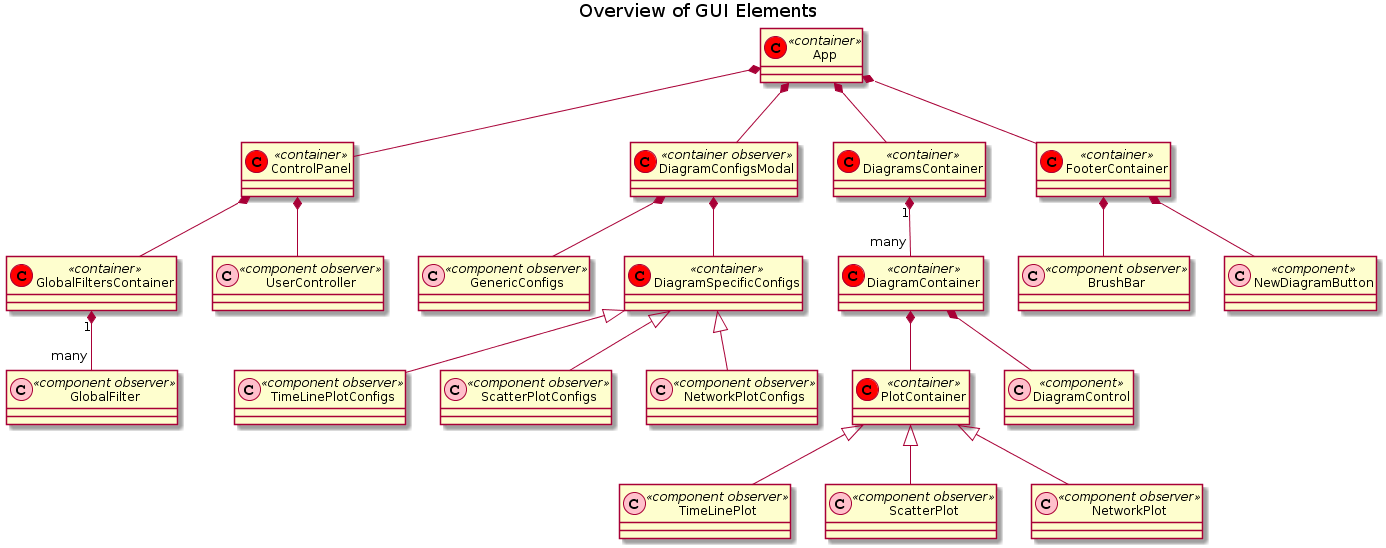
\includegraphics[max size={0.94\textheight}{\textwidth}]{images_design/overview.png}%
	\end{adjustbox}
\end{figure}

\begin{figure}[p]
	\vspace*{-2cm}
	\makebox[\linewidth]{
		\begin{adjustbox}
			{addcode={\begin{minipage}{\width}}
							{\caption{%
								This diagram shows the definitions of all representational elements.
							}
							\label{fig:component_defs}
						\end{minipage}},center}
			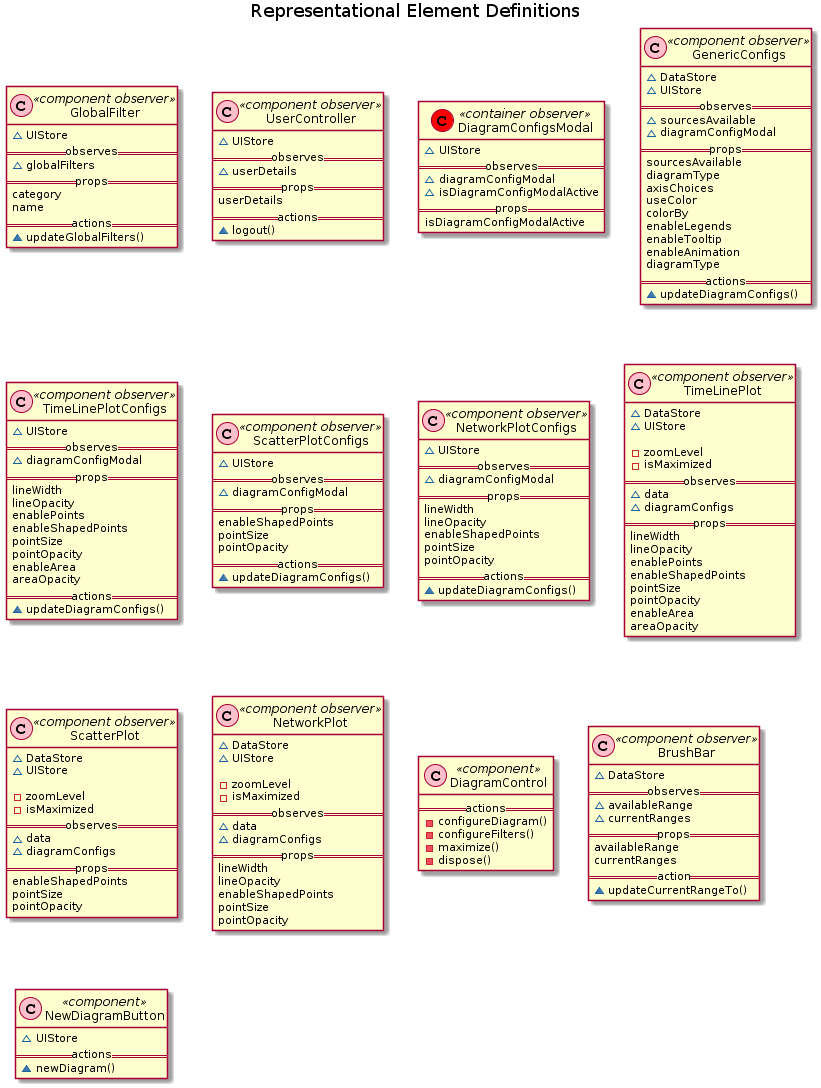
\includegraphics[max size={\textheight}{1.5\linewidth}]{images_design/componentDefs.png}%
		\end{adjustbox}
	}
\end{figure}

\begin{figure}
	\begin{adjustbox}
		{addcode={\begin{minipage}{\width}}
						{\caption{%
							This diagram shows the design of the MobX state store objects and predefined actions to mutate the states.
						}
						\label{fig:state_action_store}
					\end{minipage}}}
		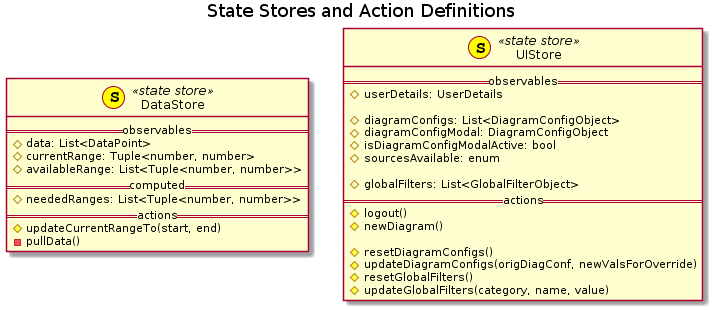
\includegraphics[max size={\textwidth}{\textheight}]{images_design/stateStoresAndActions.png}%
	\end{adjustbox}
\end{figure}

\begin{figure}
	\begin{adjustbox}
		{addcode={\begin{minipage}{\width}}
						{\caption{%
							This diagram shows the definitions of custom types that are used in the MobX state stores.
						}
						\label{fig:type_defs}
					\end{minipage}}}
		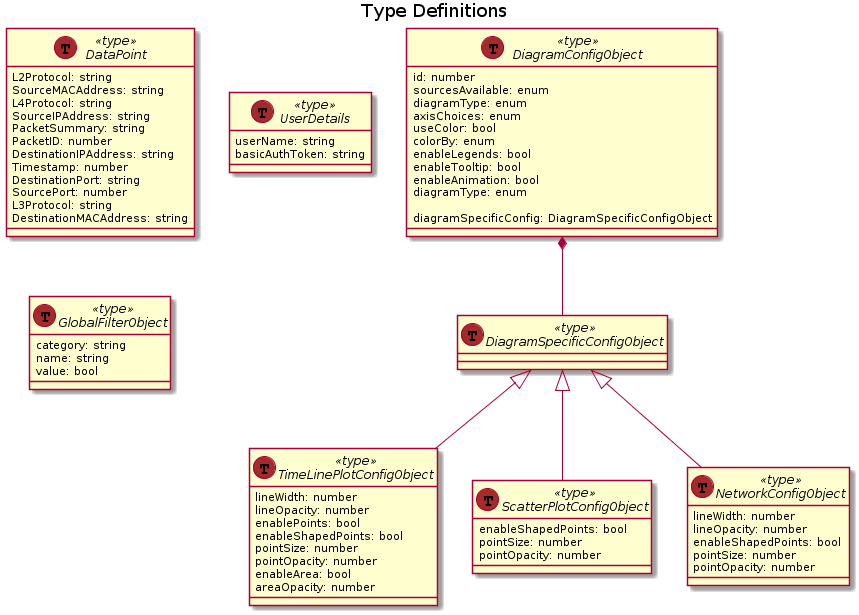
\includegraphics[max size={\textwidth}{\textheight}]{images_design/typeDefs.png}%
	\end{adjustbox}
\end{figure}

\begin{figure}[h!]
	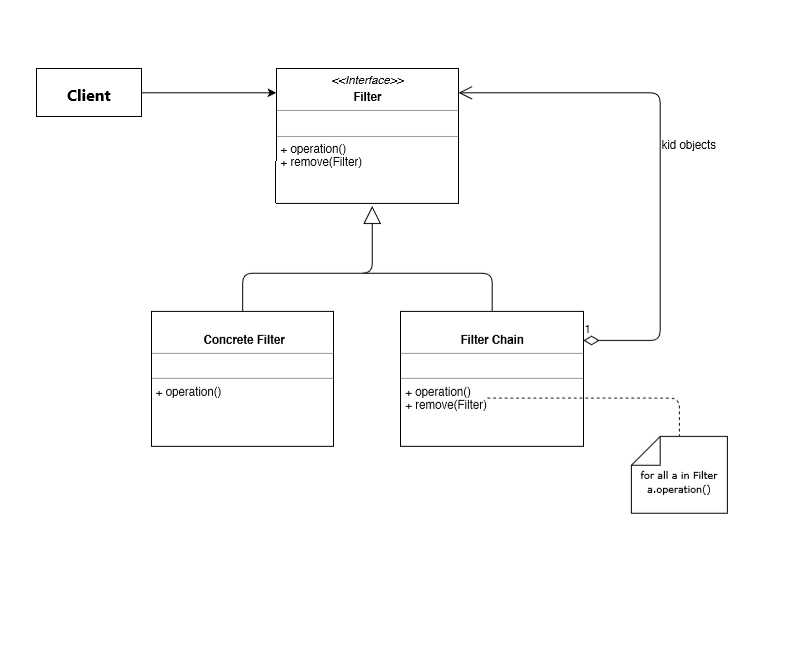
\includegraphics[max size={\textwidth}{0.9\textheight}]{images_design/clientfix.png}
	\caption{Class diagram representing the filtering chain.}
\end{figure}

\clearpage
\subsection{Sequence Diagram}

\begin{figure}[h!]
	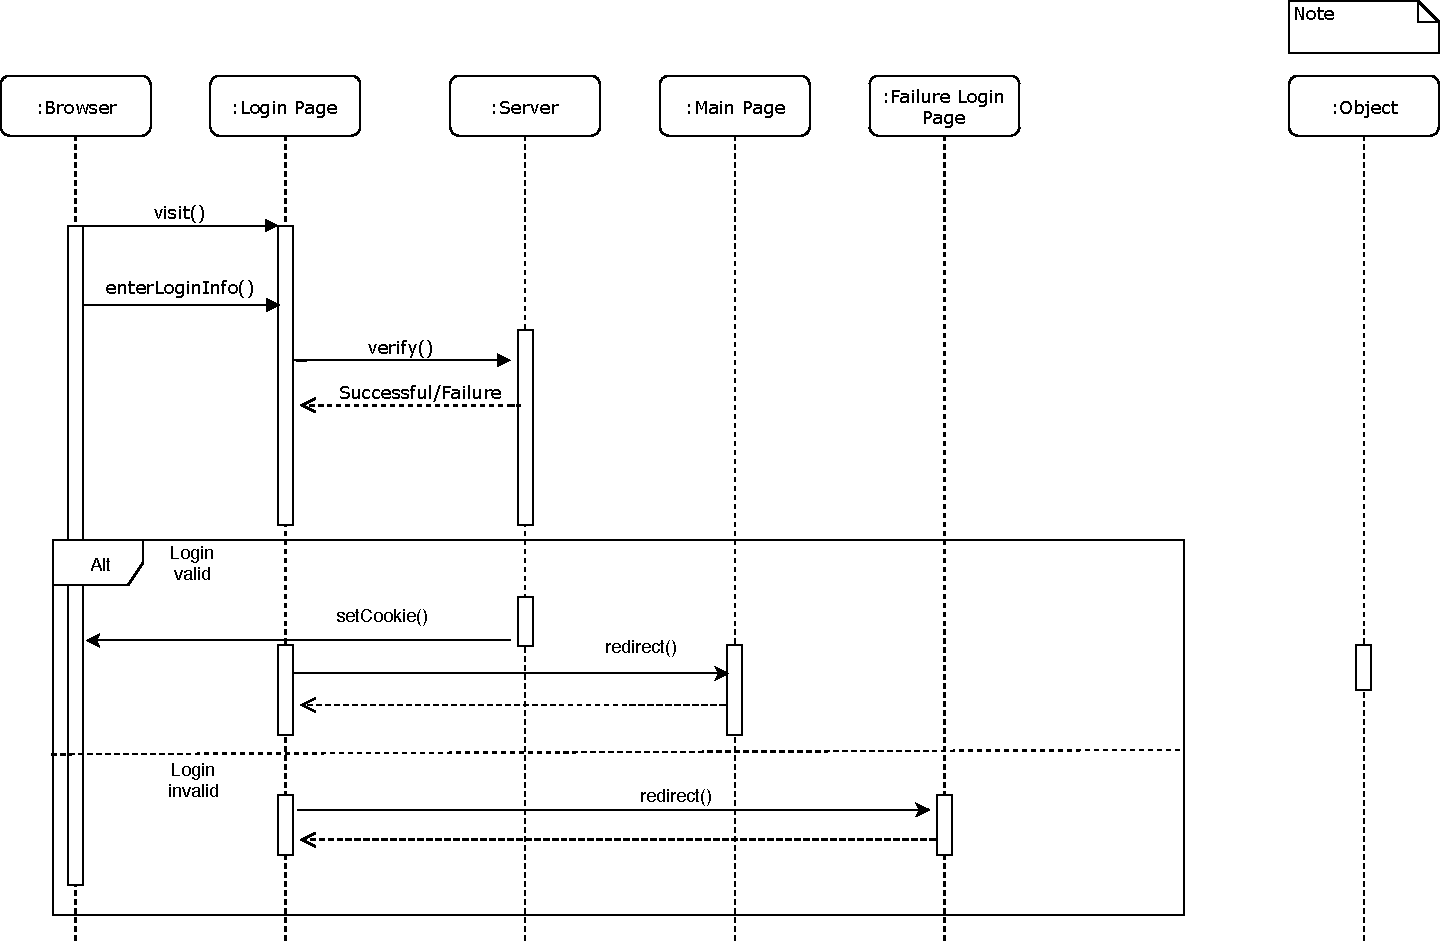
\includegraphics[max size={\textwidth}{\textheight}]{images_design/login1.pdf}
	\caption{Sequence diagram of Login Authentication System. The user credentials are transmitted via https and the server returns a token to identify the following user session.}
	\label{fig:login_https}
\end{figure}
\newpage

\begin{figure}[h!]
	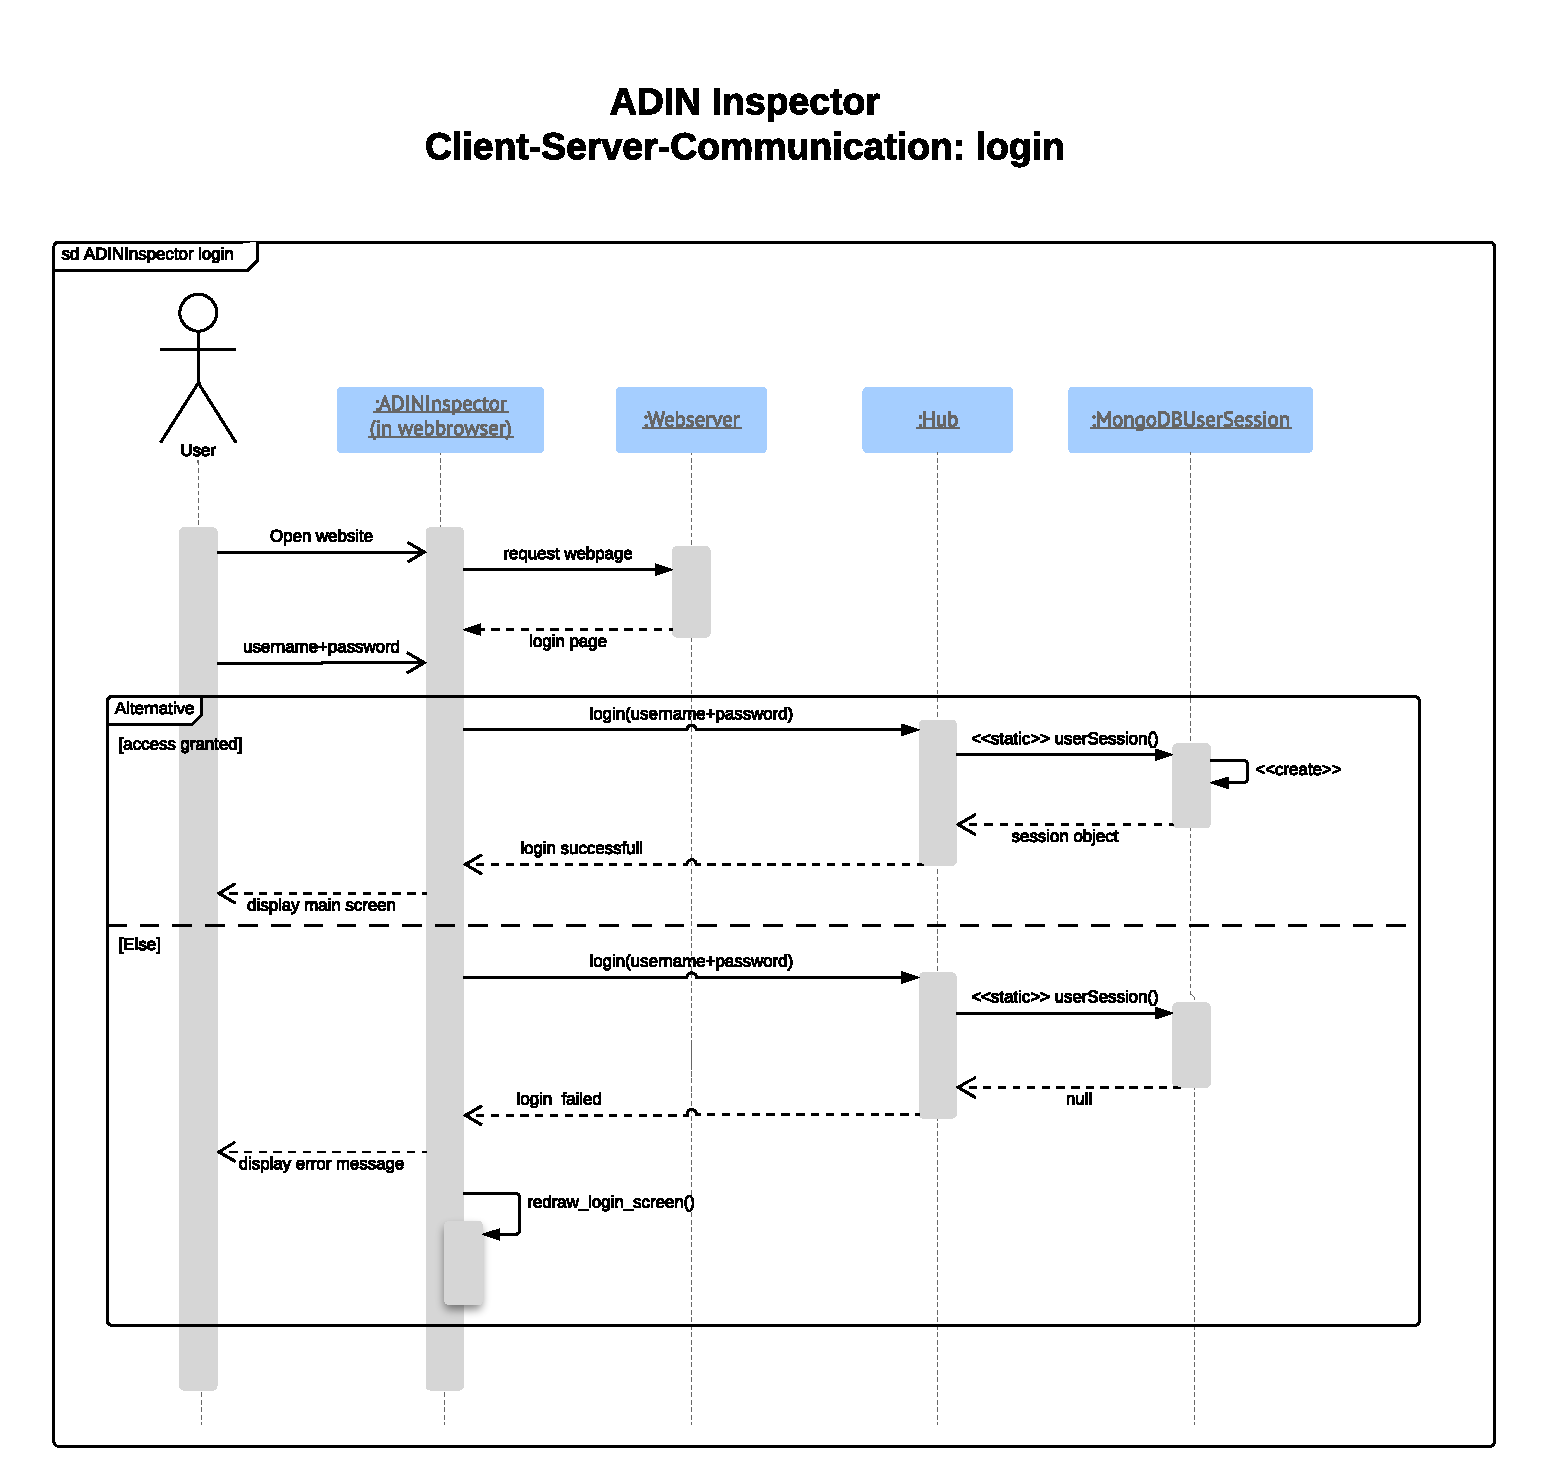
\includegraphics[max size={\textwidth}{\textheight}]{images_design/ADIN_Inspector_Client-Server-Communication-login.pdf}
	\caption{This diagram shows an alternative view of the login sequence where the user credentials are transmitted via the same encrypted WebSocket connections which is used for the following session.}
	\label{fig:login_websocket}
\end{figure}
\newpage

\begin{figure}[h!]
	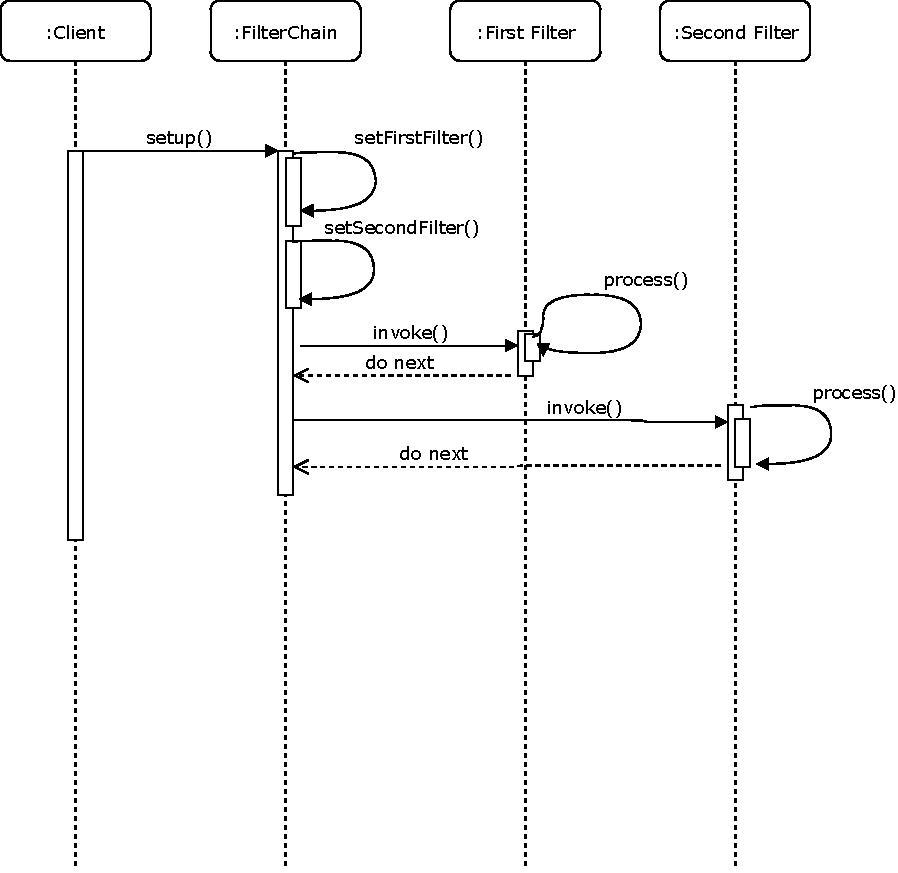
\includegraphics[max size={\textwidth}{\textheight}]{images_design/filterchain.pdf}
	\caption{Sequence diagram of chaining filters in a specific diagram.}
\end{figure}
\newpage

\begin{figure}[h!]
	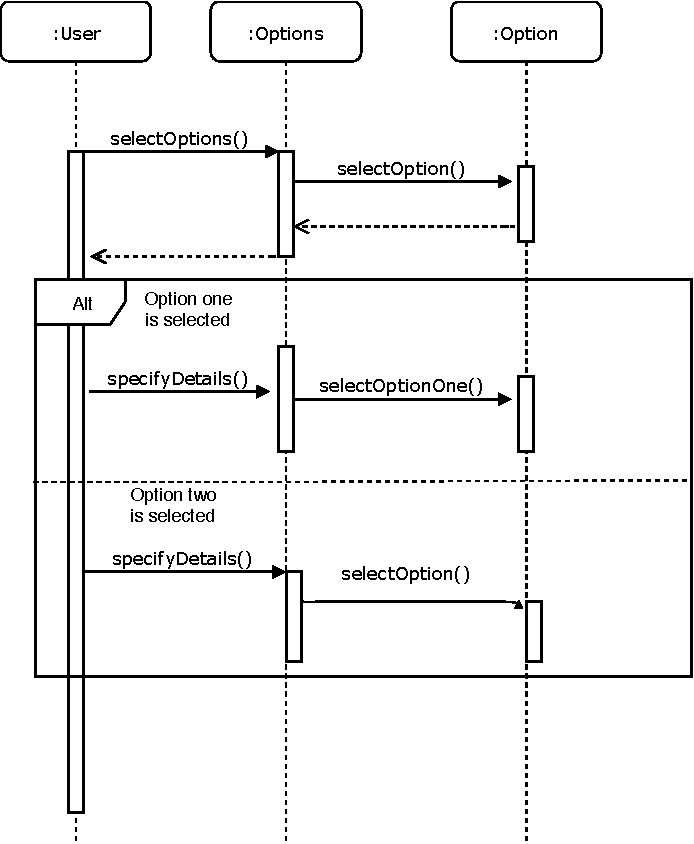
\includegraphics[max size={\textwidth}{\textheight}]{images_design/option.pdf}
	\caption{Selecting a specific option from a drop-down menu.}
\end{figure}

\begin{center}
	\begin{figure}[h!]
		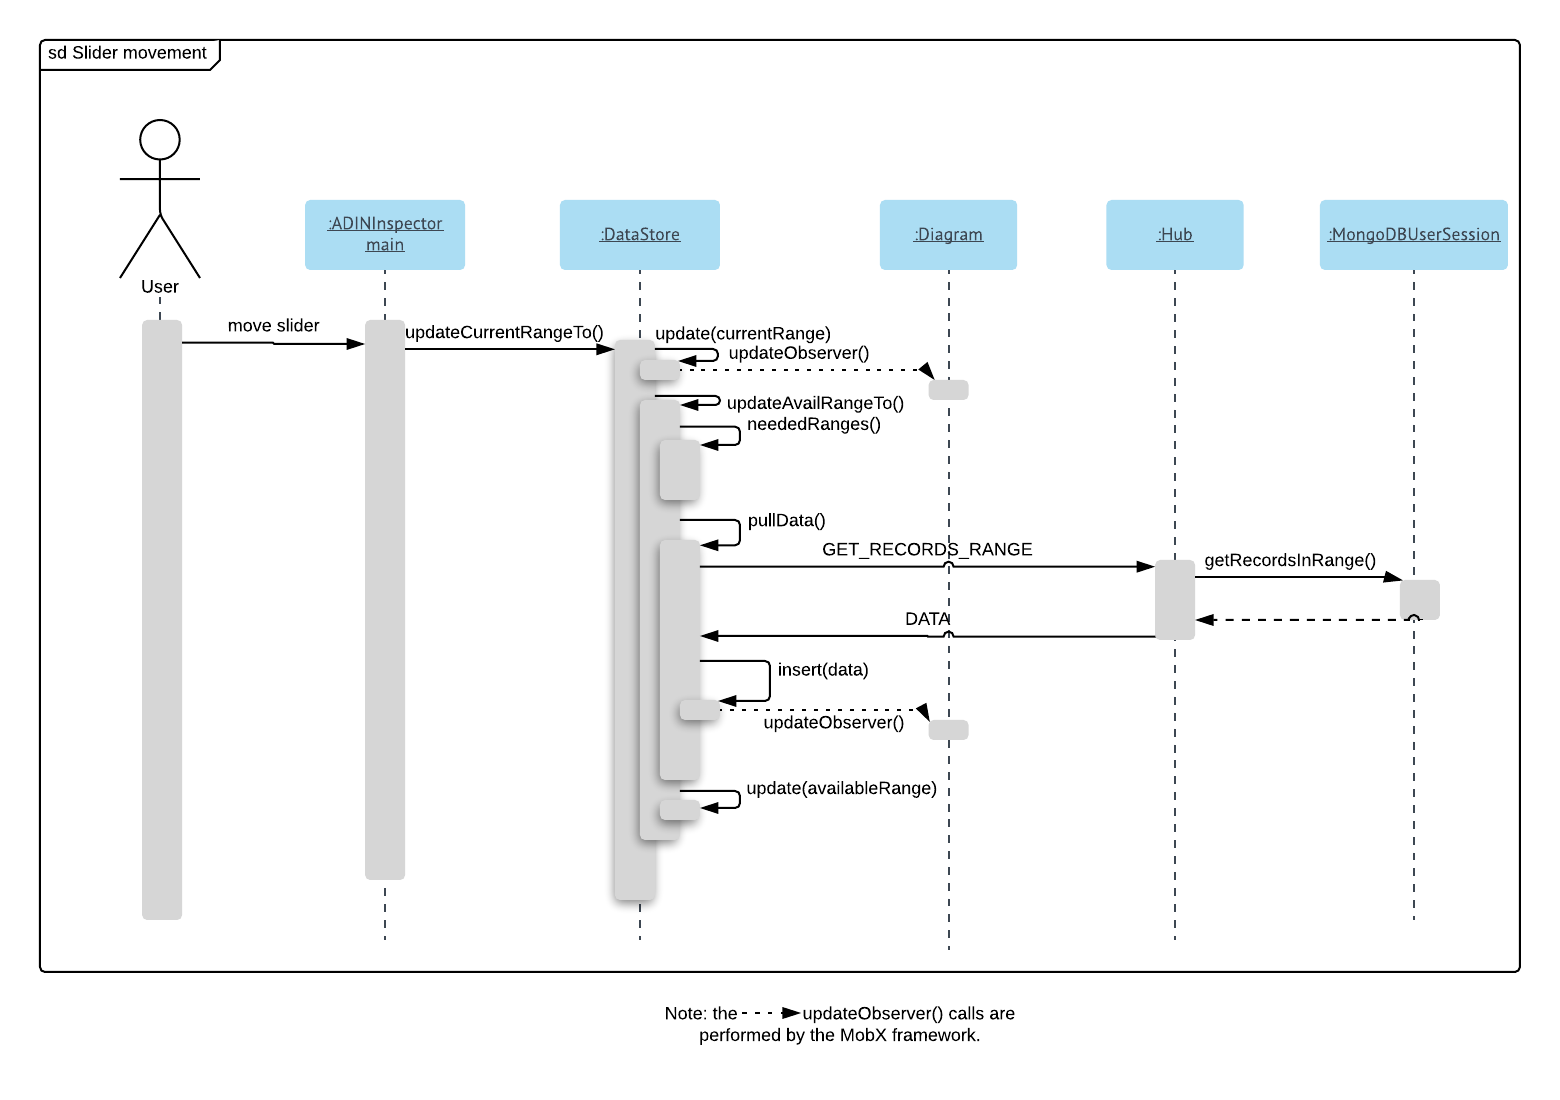
\includegraphics[width=\textwidth]{images_design/sd_frontend_comm-slider_movement.png}
		\caption{Sequence diagram showing control flow for handling a movement of the slider by the user.}
		\label{fig:sd_slider_movement}
	\end{figure}
\end{center}

\clearpage


\section{Client-server protocol}
The client (web browser) and server communicate using the encrypted WebSocket protocol (wss://).
Messages between client and server are exchanged as strings in JSON format.
Communication is typically initiated by the client. Each request has a message id which is echoed back in the response to help the sender to link the response to the request. The ids can be random, they don't have to be in a specific order.
\\
By default, all requests apart from login will be ignored.  A communication session starts with a login request that is responded to with an "OK" session control message. Within a communication session, login is ignored and all other requests can occur in arbitrary order. On receiving a logout request, the server returns into the default state, i.e logged out.\\
The user credentials that the user enters in the login web page can be transmitted in two different ways.
In the first case they are sent via https with the POST method to the web server and the server returns a token which the client (the web browser) will save in a cookie and then transmit to the server in the WebSocket session with the LOGIN\_TOKEN message to authenticate the WebSocket session (see \autoref{fig:login_https}).
In the alternative case the client opens an encrypted WebSocket connection to the server and sends the user credentials with the LOGIN message; i.e user authentication and data communication take place within the same WebSocket session (see \autoref{fig:login_websocket}).\\
All communication, including the user authentication, uses https or wss, respectively, both of which use TLS/SSL encryption. The MongoDB data base doesn't store user passwords in plaintext but stores a hashed value derived from the password.\\
Responses carrying data, specifically "data set" and "collection size", will echo back any key-value pairs that are in addition to those specified in the protocol. This allows the client to add information that will help in processing the response, e.g. when requesting several "chunks" of data that will be concatenated.
\hfill
\\
In the following list words in angle brackets ("<>") are placeholders.

\subsection{Requests from client to server:}
\begin{itemize}
	\item{login}
	      \\
	      syntax: \{"cmd": "LOGIN", "user": "<username>", "pwd": "<password>", "id": "<id>"\} \\
	      expected response: session control with key "par" having the value "LOGIN"


	\item{authentication via token}
	      \\
	      syntax: \{"cmd": "AUTH", "token": "<token>", "id": "<id>"\} \\
	      expected response: session control with "par": "AUTH"

	\item{logout}
	      \\
	      syntax: \{"cmd": "LOGOUT", "id": "<id>"\} \\
	      expected response: session control with "par": "LOGOUT"

	\item{getAvailableCollections}
	      \\
	      syntax: \{"cmd": "GET\_AV\_COLL", "id": "<id>"\} \\
	      expected response: list of collections

	\item{getCollectionSize(collection)}
	      \\
	      syntax: \{"cmd": "GET\_COLL\_SIZE", "par": "<collection>", "id": "<id>"\} \\
	      where <collection> is the name of a collection\\
	      expected response: collection size

	\item{getStartRecord(collection)}
	      \\
	      syntax: \{"cmd": "GET\_START", "par": "<collection>", "id": "<id>"\} \\
	      expected response: single data point, with "idx": "start" and key "data" containing the first data point of the given collection

	\item{getEndRecord(collection)}
	      \\
	      syntax: \{"cmd": "GET\_END", "par": "<collection>", "id": "<id>"\} \\
	      expected response: single data point, with "idx": "end" and key "data" containing the last data point of the given collection

	\item{getEndpoints(collection)}
	      \\
	      syntax: \{"cmd": "GET\_ENDPOINTS", "par": "<collection>", "id": "<id>"\} \\
	      expected response: data endpoints, with the key "data" containing a array consisting of the first and the last data point of the given collection

	\item{getCollection(collection)}
	      \\
	      syntax: \{"cmd": "GET\_COLL", "par": "<collection>", "id": "<id>"\} \\
	      expected response: data set

	\item{getRecordsInRange(collection, key, start, end)}
	      \\
	      syntax: \{"cmd": "GET\_RECORDS\_RANGE", "par": "<collection>", "key": "<keyvalue>", "start": "<startvalue>", "end": "<endvalue>", "id": "<id>"\} \\
	      where <key> is the name of a key in the given collection and <startvalue> and <endvalue> are valid values for this key\\
	      expected response: data set, where key "data" contains all data points (i.e. records) from the given collection for which the given key is in the interval [start, end).

	\item{getRecordsInRangeSize(collection, key, start, end)}
	      \\
	      syntax: \{"cmd": "GET\_RECORDS\_RANGE\_SIZE", "par": "<collection>", "key": "<keyvalue>", "start": "<startvalue>", "end": "<endvalue>", "id": "<id>"\} \\
	      expected response: collection size, where the key "par" gives the number of data points that would be returned by a getRecordsInRange() request with the same arguments.

\end{itemize}

\newpage

\subsection{Responses from server to client:}
\begin{itemize}
	\item{session control}
	      \\
	      syntax: \{"cmd": "SESSION", "par": "<specifier>", "status": "<status>", msg": "<message>", "id": "<id>"\} \\
	      where <specifier> is one of "LOGIN", "AUTH", oder "LOGOUT", <status> is either "OK" or "FAIL" and <message> is a string, e.g. an error message\\
	      "OK" as status for "LOGIN" and "AUTH" indicates a successful login, i.e. that the client session has started. "OK" as status for "LOGOUT" indicates that the server had ended the session and the user has been logged out.

	\item{list of collections}
	      \\
	      syntax: \{"cmd": "LIST\_COLL", "par": ["<collection>"], "id": "<id>"\} \\
	      where <collection> is the name of a collection

	\item{collection size}
	      \\
	      syntax: \{"cmd": "COLL\_SIZE", "name": "<name>", "key", "", "par": "<size>", "id": "<id>"\} \\
	      syntax: \{"cmd": "COLL\_SIZE", "name": "<name>", "key", "<key>", "start": "<start>", "end": "<end>", "par": "<size>", "id": "<id>"\} \\
	      where <name> is the name of a data collection and <size> is the number of data points in this collection . If <key> is not an empty string, then <size> will be the number of data points from the given collection for which the key value is in the interval [<start>, <end>).

	\item{single data point}
	      \\
	      syntax: \{"cmd": "DATASINGLE", "name": "<collection>", "idx": "<idx>", "data": "<data>", "id": "<id>"\} \\
	      where <collection> is the name of a collection, "idx" has either the value "start" or "end", and <data> is a string representing a single data point in JSON format.

	\item{data endpoints}
	      \\
	      syntax: \{"cmd": "DATA\_ENDPOINTS", "name": "<collection>", "data": ["<start>", "<end>"], "id": "<id>"\} \\
	      where <collection> is the name of a collection and <start> and <end> are the first and last data point of this collection.

	\item{data set}
	      \\
	      syntax: \{"cmd": "DATA", "name": "<name>", "key": "", "data": [<record>], "id": "<id>"\} \\
	      syntax: \{"cmd": "DATA", "name": "<name>", "key": "<key>", "start": "<start>", "end": "<end>", "data": [<record>], "id": "<id>"\} \\
	      where <name> is the name of a data collection and each record is a JSON object describing a data point from this collection. If <key> is not an empty string, then the data array will contain those data points from the given collection for which the key value is in the interval [<start>, <end>).
\end{itemize}

\section{Back-End}
This subsection deals with the back-end of the ADIN INSPECTOR. How the system deals with client http calls, and how kafka interacts with the system.
An overview of the system can be seen in \autoref{fig:class_back_end}. Smaller subsections have been expanded in \autoref{fig:class_back_end_init}, \autoref{fig:class_back_end_mongo}, \autoref{fig:class_back_end_hub}.

The connection to the client is handled in the class Hub which contains handlers for the network interface. This class uses a separate class (ClientProtocolHandler) to parse and handle requests from the handler. This setup is according to the strategy design pattern and allows easily modifying or even replacing the client server-protocol.
The Hub class and the ClientProtocolHandler access the database via an object that implements the IUserSession interface and encapsulates the database session. Currently there is only an implementation for MongoDB access (MongoDBUserSession), but the abstraction via the IUserSession interface allows to add classes that offer access to Kafka or other databases.
Classes that implement IUserSession are instantiated with a factory Method (UserSession()) which guarantees that the returned object represents a successfully logged in database session.


\subsection{Class Diagram}
The overview in  \autoref{fig:class_back_end} shows a number of classes and their interaction with each other. What follows is a more in-depth view of what each component of this diagram does, what data it stores and how it fits into the overarching architecture.

\clearpage
\begin{figure}[h!]
	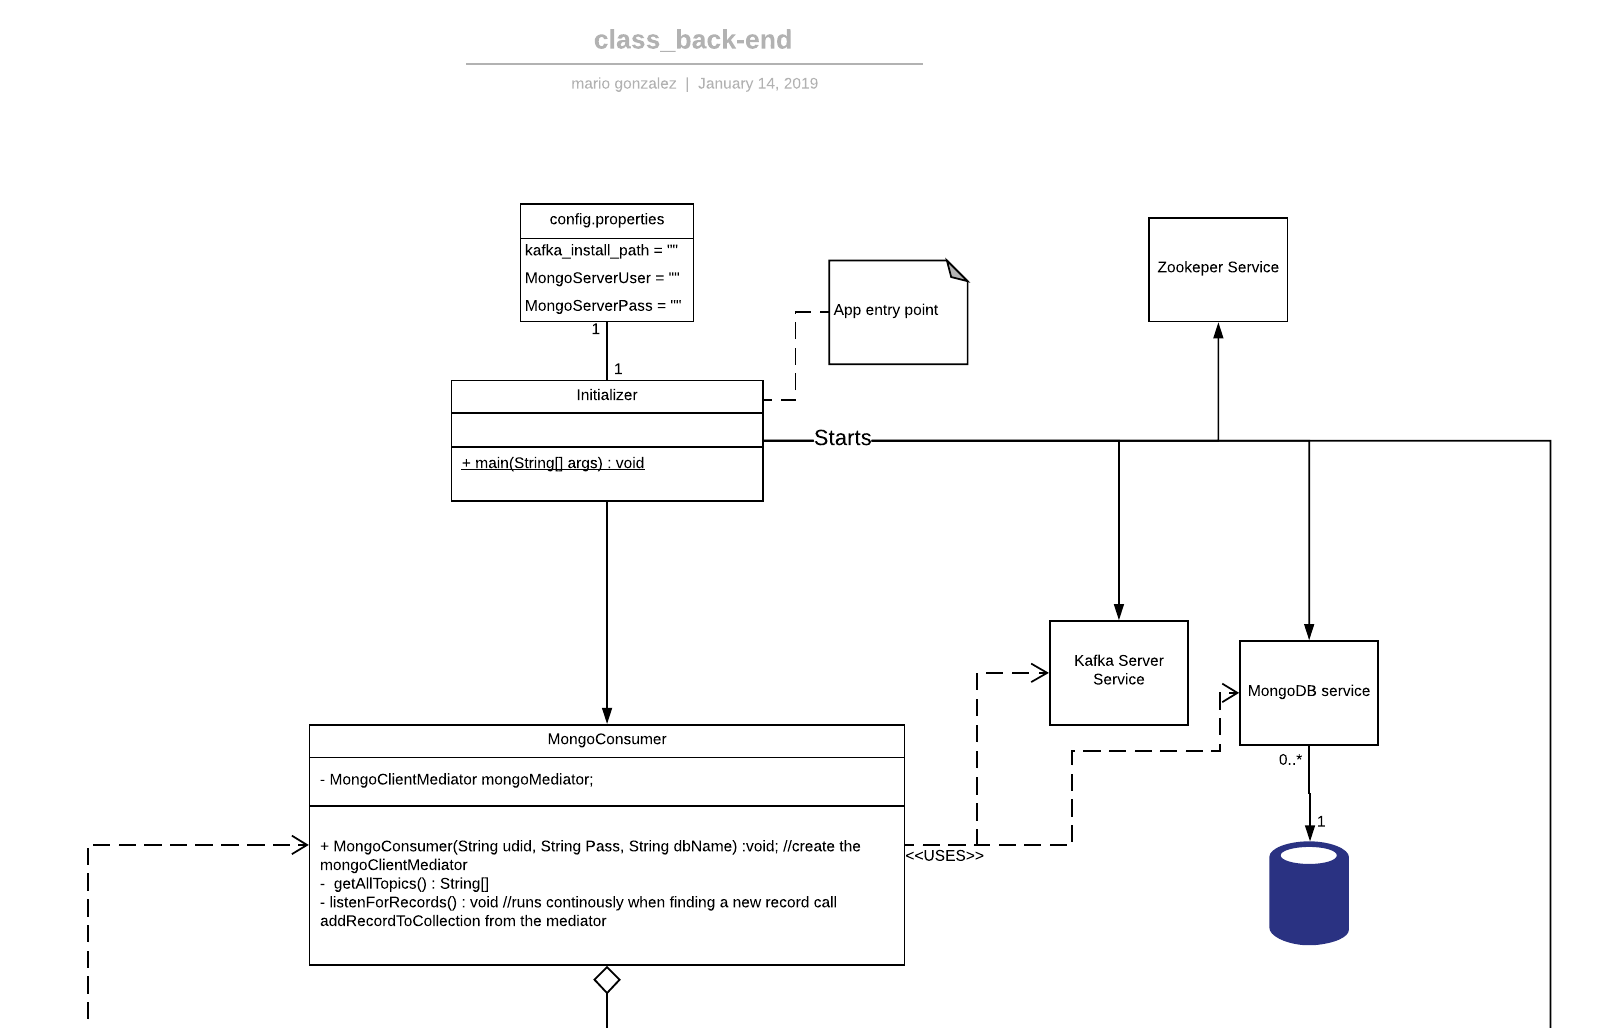
\includegraphics[max size={\textwidth}{\textheight}]{images_design/class_back-end_init.png}
	\caption{The classes involved in the initialization setup}
	\label{fig:class_back_end_init}
\end{figure}


\begin{itemize}

	\item[•] Config properties file
	      \\The config file is stored alongside the built application .jar file and contains the path to the Kafka installation folder, the user name and password of a mongoDB account with the highest level of access and the name of the database.

	\item[•]Initializer
	      \\Methods:
	      \begin{itemize}
		      \item[-]main
		            \\ parameters: String of arguments from the console
		            \\ returns: void
		            \\ App entry point.
		            \\ We load the config.properties life and use the path provided to start the zookeeper, kafka and mongodb services
	      \end{itemize}


	\item[•]MongoConsumer
	      \\The Mongo Consumer, as the name implies, consumes all messages from all topics in the Kafka messaging system. Once a message is found it is passed along to the Mongo Client for further processing.
	      \\Attributes
	      \begin{itemize}
		      \item[-]clientMediator
		            \\Type : MongoClientMediator
		            \\ An instance of the Mongo Client Mediator, created with the credentials from the config file.
	      \end{itemize}
	      Methods
	      \begin{itemize}
		      \item[-]MongoConsumer constructor
		            \\parameters: user name and password of a mongoDB account with the highest level of access.
		            \\ Initializes the MongoClient variable and calls listenForRecords();
		      \item[-]getAllTopics
		            \\parameters: none
		            \\returns: an array of strings containing all the available kafka Topics.
		            \\Asks the kafka server service which topics exists.
		      \item[-]listenForRecords
		            \\parameters: none
		            \\returns: void
		            \\This Method first calls getAllTopics and uses the array of topics to poll the kafka server for new messages.
		            \\If new messages are found then the messages are passed to the Mongo Mediator for adding them to the Database.
		            \\If no new messages are found for a topic notify the Mongo Mediator that the collection tied to the topic is ready for pre-processing.
	      \end{itemize}



	      \begin{figure}[h!]
		      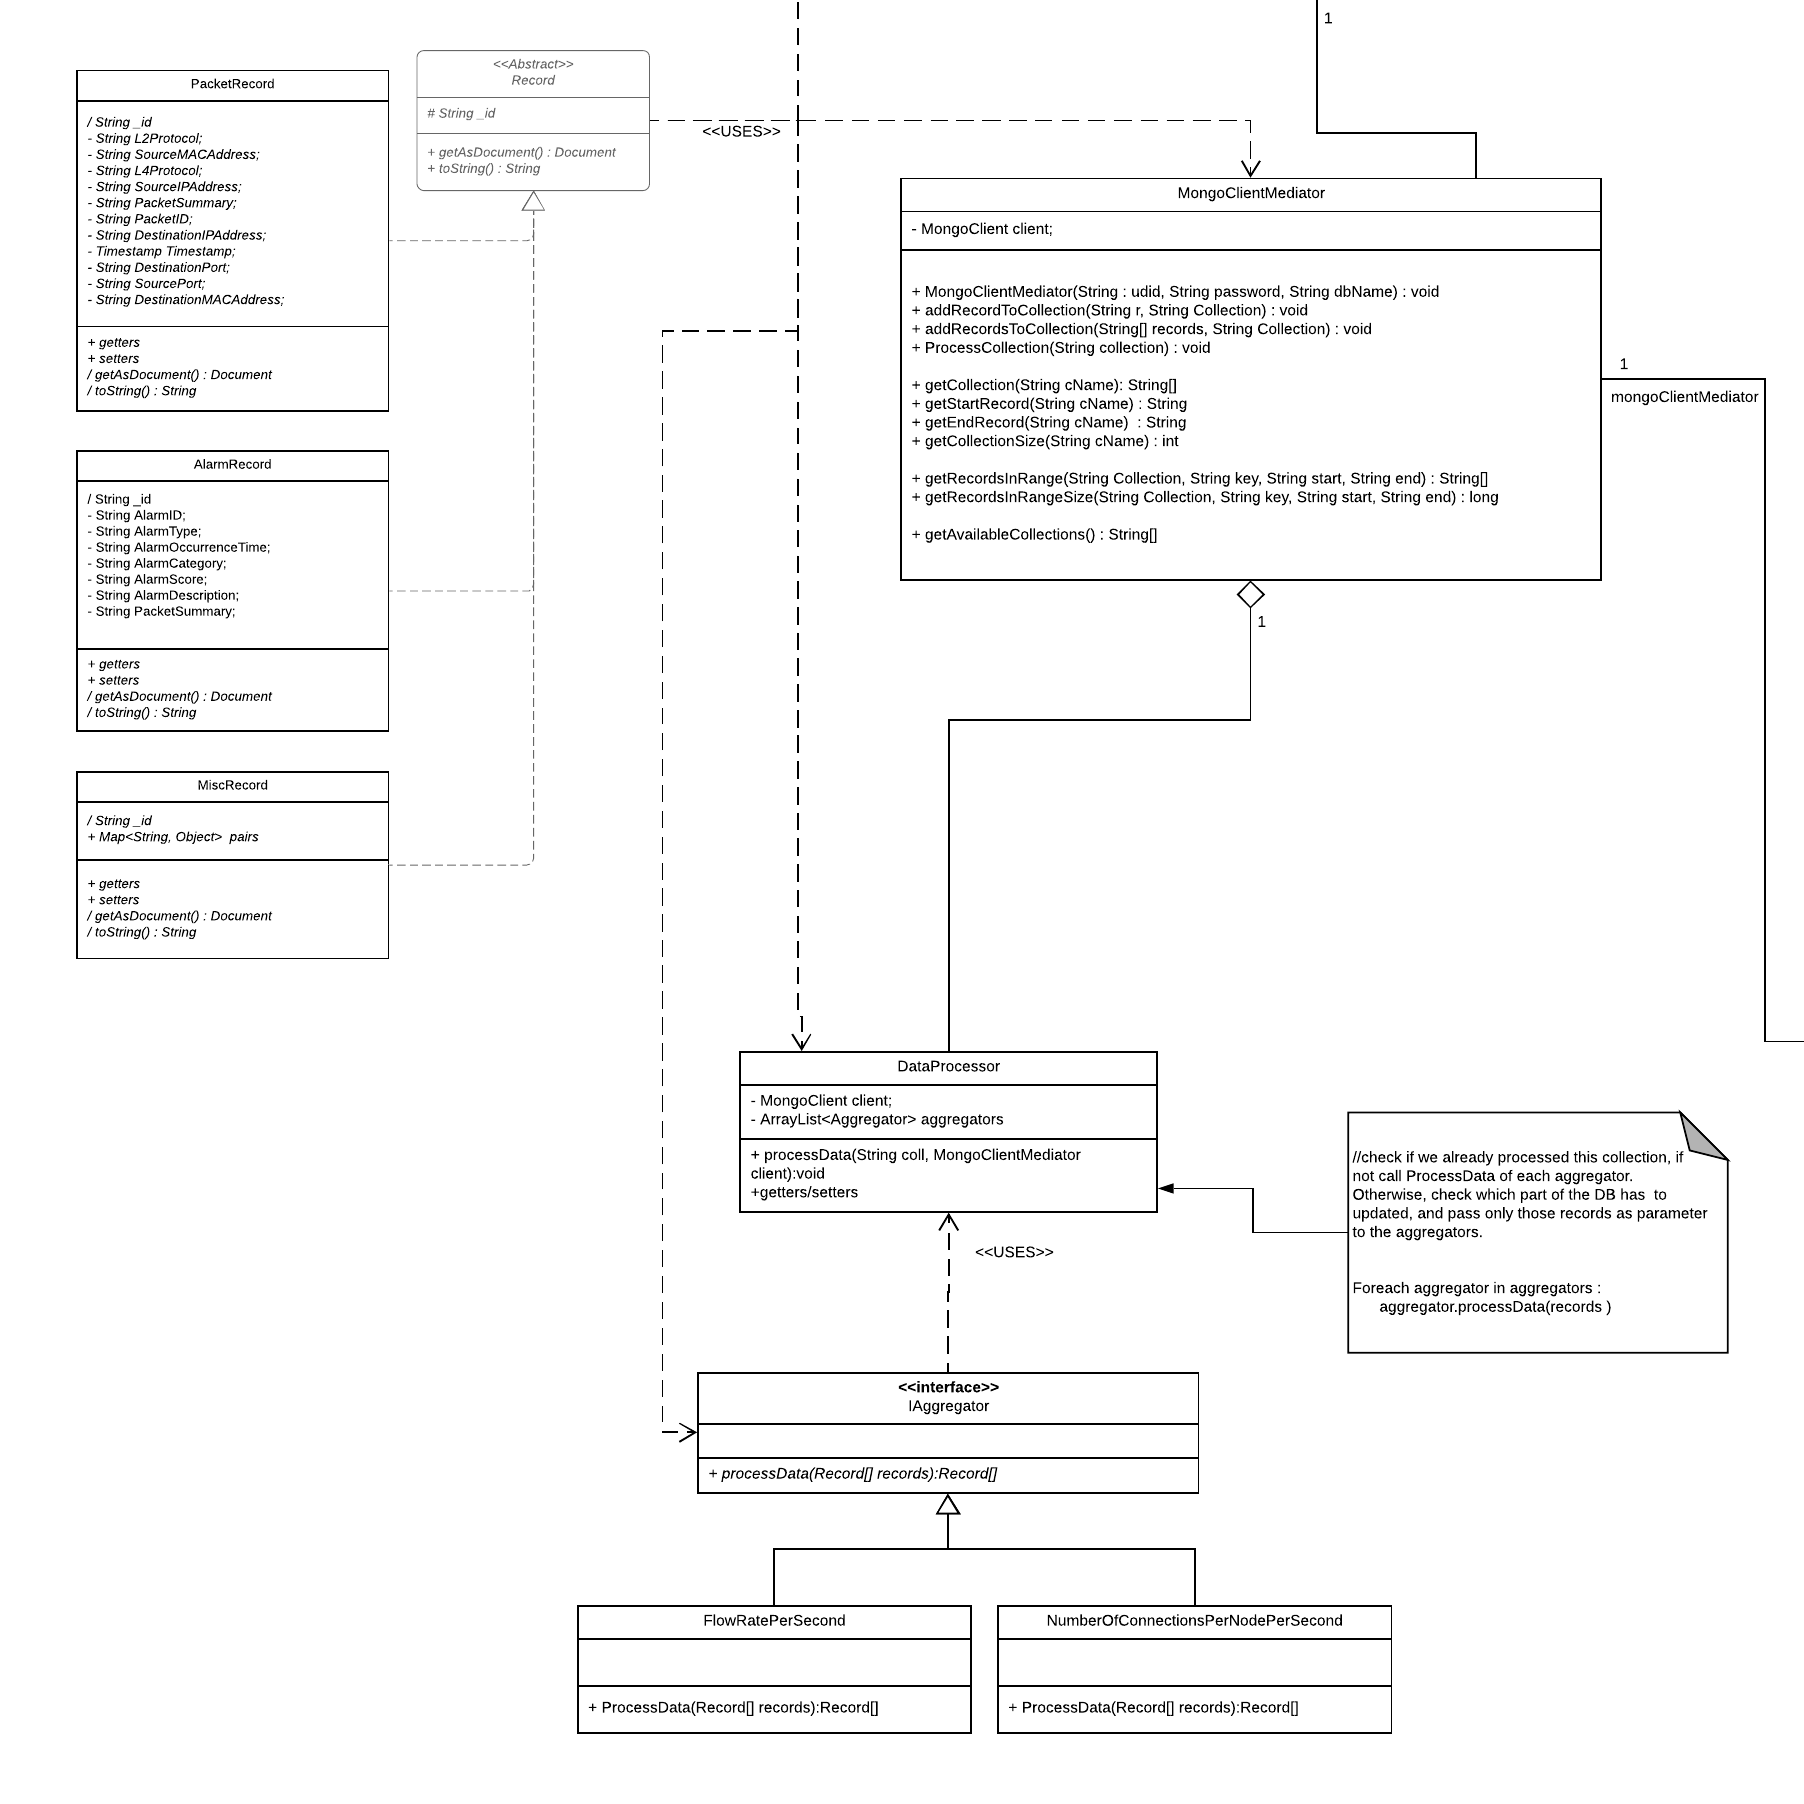
\includegraphics[max size={\textwidth}{\textheight}]{images_design/class_back-end_mongo.png}
		      \caption{The classes involved in reading and writing data into the database}
		      \label{fig:class_back_end_mongo}
	      \end{figure}
	      \clearpage
	\item[•]MongoClientMediator
	      This object serves as a nexus between the users who want to get data out of the database and the consumer and dataProcessor who want to add data into the database. This class encapsulates the mongo client from the mongo API. This means that any user wanting to sign in has to have valid credentials in the database, effectively relegating UAC to mongoDB.
	      \\Attributes
	      \begin{itemize}
		      \item[-] client
		            \\type: MongoClient
		            \\ An instance of the Mongo Client from the official java API.
		      \item[-] dataProc
		            \\ A reference to the data processor class for this client.
	      \end{itemize}
	      Methods
	      \begin{itemize}
		      \item[-]MongoClientMediator constructor
		            \\parameters: Username and password
		            \\Initializes the client variable, throws an error if the user is not found.

		      \item[-]addRecordToCollection
		            \\parameters: String representation of a record in json format
		            \\String name of the collection it should be added to.
		            \\returns: void
		            \\Converts the json string into a java object, then to a bson document and uses the mongoAPI to insert it into the database.

		      \item[-]addRecordsToCollection
		            \\parameters: String Array of records to be added to a collection
		            \\String name of the collection it should be added to.
		            \\returns: void
		            \\for each oneof the members of the array call addRecordToCollection

		      \item[-]ProcessCollection
		            \\parameters: String, name of a collection
		            \\returns: void
		            \\signal the data processor to start the processing of a collection

		      \item[-]getCollection
		            \\parameters: String, name of a collection
		            \\returns: String array containing all entries of the collection

		      \item[-]getStartRecord
		            \\parameters: String, name of a collection
		            \\returns: the first entry of the collection as a String.

		      \item[-]getEndRecord
		            \\parameters: String, name of a collection
		            \\returns: the last entry of the collection as a String.

		      \item[-]getCollectionSize
		            \\parameters: String, name of a collection
		            \\returns: the number of entries in the collection as int

		      \item[-]getRecordsInRange
		            \\parameters: String, name of the collection to query
		            \\String, key of the parameter used for filtering
		            \\String start and end ranges for the filtering
		            \\returns: String array containing all entries of the collection within that range
		            \\this Method is very general to allow for flexibility.For example by letting the key be, SourceIPaddresses, or a timeStamp.

		      \item[-]getRecordsInRangeSize
		            \\parameters: String, name of the collection to query
		            \\String, key of the parameter used for filtering
		            \\String start and end ranges for the filtering
		            \\returns: number of elements matching the range as int
		      \item[-]getAvailableCollections
		            \\parameters: -
		            \\returns: String array with collection names
		            \\Returns an array with the names of the collections available to the current user.


	      \end{itemize}

	\item[•]Record
	      \\Every message that comes from kafka and needs to be added to the database has its own Record class that inherit from this one.
	      \\Every single class that inherits needs to be able to, using reflection, convert itself into a Bson Document where every variable is a key Value pair of the name of the variable and its associated value.
	      \\Attributes
	      \begin{itemize}
		      \item[-] id
		            \\type: String
	      \end{itemize}
	      Methods
	      \begin{itemize}
		      \item[-]getAsDocument()
		            \\parameters: none
		            \\returns: A Document, containing every variable of any class inheriting from this one.
		            \\This function checks for every variable, gets its name and value as a string and adds it to the document that it eventually returns.
	      \end{itemize}

	\item[•]PacketRecord
	      \\Inheriting from Record, this class contains the variables that match the json string obtained from kafka.
	      \\Attributes
	      \begin{itemize}
		      \item[-] id
		            \\type: String
		            \\this id is used for determining the ordering when saving to mongoDB, it's the offset of the message in the kafka messaging queue. inherited from Record
		      \item[-] client
		            \\type: String
		      \item[-] L2Protocol
		            \\type: String
		      \item[-] SourceMACAddress
		            \\type: String
		      \item[-] L3Protocol
		            \\type: String
		      \item[-] L4Protocol
		            \\type: String
		      \item[-] SourceIPAddress
		            \\type: String
		      \item[-] PacketSummary
		            \\type: String
		      \item[-] DestinationIPAddress
		            \\type: String
		      \item[-] Timestamp
		            \\type: String
		      \item[-] DestinationPort
		            \\type: String
		      \item[-] SourcePort
		            \\type: String
		      \item[-] DestinationMACAddress
		            \\type: String

	      \end{itemize}

	      Methods
	      \begin{itemize}
		      \item[-]getters / setters
		            \\parameters: variable
		            \\returns: variable type
		            \\Each variable has its getters and setter methods.
	      \end{itemize}

	\item[•]AlarmRecord
	      \\Inheriting from Record, this class contains the variables that match the json string obtained from kafka.
	      \\Attributes
	      \begin{itemize}
		      \item[-] id
		            \\type: String
		      \item[-] AlarmID
		            \\type: String
		      \item[-] AlarmType
		            \\type: String
		      \item[-] AlarmOccurrenceTime
		            \\type: String
		      \item[-] AlarmCategory
		            \\type: String
		      \item[-] AlarmScore
		            \\type: String
		      \item[-] AlarmDescription
		            \\type: String
		      \item[-] PacketSummary
		            \\type: String

	      \end{itemize}
	      Methods
	      \begin{itemize}
		      \item[-]getters / setters
		            \\parameters: variable
		            \\returns: variable type
		            \\Each variable has its getters and setter methods.
	      \end{itemize}

	\item[•]MiscRecord
	      \\Inheriting from Record, this class is used by the data processor as an 'in-between' state before saving to the database. As well as an extension point for adding more types of records into the database programatically in the future.
	      \\Refer to the data processor class for further data on the key value pairs.
	      \\Attributes
	      \begin{itemize}
		      \item[-] pairs
		            \\ A Map of strings to Objects to store any 1 to many relationships
	      \end{itemize}
	      Methods
	      \begin{itemize}
		      \item[-]getters / setters
		            \\parameters: none
		            \\returns: variable type
		            \\Each variable has its getters and setter methods.
	      \end{itemize}

	\item[•]DataProcessor
	      \\This class is a mediator for each one of our data aggregators used for extraciton of features from the raw data stored in mongoDB.
	      \\ We might want to hve multiple data processors for chaining different aggregators together or to split up the work into mutliple threads. This is dependant on further performance testing.
	      \\Attributes
	      \begin{itemize}
		      \item[-] client
		            \\ an instance of the associated mongoClient that requested the data aggregation
		      \item[-] aggregators
		            \\ A Arraylist containing all the aggregators to be applied on a collection.
	      \end{itemize}
	      Methods
	      \begin{itemize}
		      \item[-]getters / setters
		      \item[-]processData
		            \\parameters: variable
		            \\returns: variable type
	      \end{itemize}
	\item[•] IAggregator
	      \\This interface is the building block for every aggregator to be applied to data
	      \\Attributes
	      Methods
	      \begin{itemize}
		      \item[-]processData
		            \\parameters: Records array of the records to be processed
	      \end{itemize}

	\item[•] FlowRatePerSecond
	      \\Implements IAggregator. This calculates, per port, the outgoing and incoming connections.
	      A record processed by this aggregator is stored in a collection as follows:
	      \begin{verbatim} 
		  Name of collection: collectionName\_FlowratePerSec
		  structure of record as json:
		   {
		  "date" : \{" date" " Unix_Timestamp  } 
		  rounded down to the second this record points to.
		  Connections : [
		  { Port: "portNumer", "InOut" : " In/Out ", count : "Number" }
		  { Port: "portNumer", "InOut" : " In/Out ", count : "Number" }
		  ...
		  
		  ] This array has an entry per port if the port communicated that second. 
		  Precomputing this allows us to stream whenever the client needs the information 
		  for a specific node.
		}
	      \end{verbatim}
	      Methods
	      \begin{itemize}
		      \item[-]processData
		            \\parameters: Records array of the records to be processed
		            \\ specific imlpementation left to the classes implementing this interface
	      \end{itemize}

	\item[•] NumberOfConnectionsPerNodePerSecond
	      \\Implements IAggregator. This calculates the outgoing and incoming connections.
	      A record processed by this aggregator is stored in a collection as follows:
	      \begin{verbatim} 
		  Name of collection: collectionName\_FlowratePerSec
		  structure of record as json:
		   {
		  "date" : \{" date" " Unix_Timestamp  } 
		  rounded down to the second this record points to.
		  Connections : [
		  { Port: "portNumer", count : "Number" }
		  { Port: "portNumer", count : "Number" }
		  ...
		  
		  ] This array has an entry per port if the port communicated that second. 
		  Precomputing this allows us to stream whenever the client needs the information 
		  for a specific node.
		}
	      \end{verbatim}
	      Methods
	      \begin{itemize}
		      \item[-]processData
		            \\parameters: Records array of the records to be processed
	      \end{itemize}

	      \begin{figure}[h!]
		      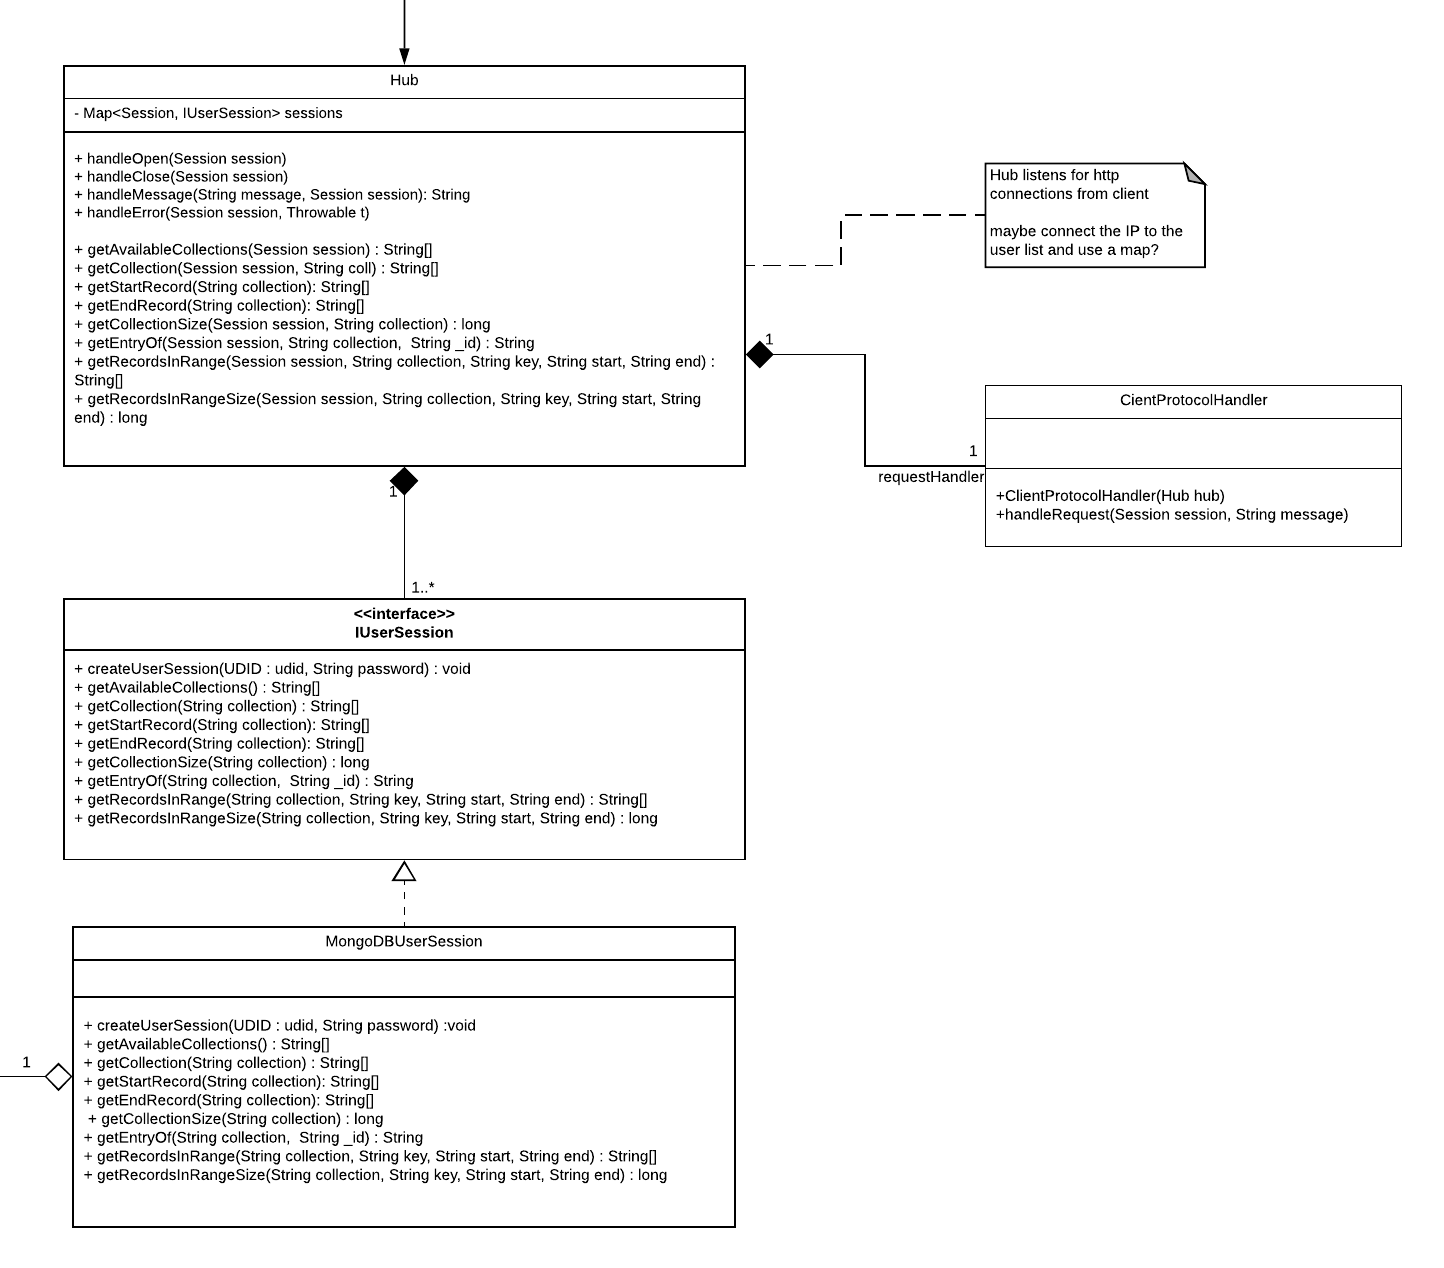
\includegraphics[max size={\textwidth}{\textheight}]{images_design/class_back-end_hub.png}
		      \caption{The classes involved in the communication between the server and the client}
		      \label{fig:class_back_end_hub}
	      \end{figure}
	      \clearpage
	\item[•]Hub
	      \\
	      This class implements the network handlers for the WebSocket connection to the client. It also has wrapper methods that delegate the database commands to the appropriate IUserSession object.
	      \\Attributes
	      \begin{itemize}
		      \item[-]requestHandler
		            \\Type : ClientProtocolHandler
		            \\The strategy object we call for the actual parsing of the client requests.
		      \item[-]sessions
		            \\Type : map<Session, IUserSession>
		            \\A map that connects a client communication session to a database session.  A non-null entry represents a successfully logged in user session.
	      \end{itemize}
	      Methods
	      \begin{itemize}
		      \item[-]handleOpen
		            \\parameters: Session session - the current session
		            \\returns: void
		            \\Event handler for the start of WebSocket connection.
		      \item[-]handleClose
		            \\parameters: Session session - the current session
		            \\returns: void
		            \\Event handler for closing a connection.

		      \item[-]handleMessage
		            \\parameters: String message - the message that we received from the client
		            \\Session session - the current session
		            \\returns: String - the response to be sent to the client
		            \\Event handler for receiving a message. The message is passed to the ClientProtocolHandler.

		      \item[-]handleError
		            \\parameters: Session session - the current session
		            \\Throwable t - the exception that occurred
		            \\returns: void
		            \\Event handler for errors/exceptions during communication.
		      \item[-]createUserSession
		            \\parameters: Session session - the current session
		            \\String username - the user id to login with
		            \\String password - the password
		            \\returns: IUserSession
		            \\Delegate to the IUserSession method to instantiate a new UserSession and log in into the database using the given credentials.

		      \item[-]getAvailableCollections
		            \\parameters: Session session - the current session
		            \\returns: String array with collection names
		            \\Returns an array with the names of the collections available to the current user.

		      \item[-]getCollection
		            \\parameters: Session session - the current session
		            \\String - name of a collection
		            \\returns: String array containing all entries of the collection

		      \item[-]getStartRecord
		            \\parameters: String, name of a collection
		            \\returns: the first entry of the collection as a String.

		      \item[-]getEndRecord
		            \\parameters: String, name of a collection
		            \\returns: the last entry of the collection as a String.

		      \item[-]getCollectionSize
		            \\parameters: Session session - the current session
		            \\String collection - the collection to query
		            \\returns: long - the number of records
		            \\Returns the number of records in the specified collection.

		      \item[-]getRecordsInRange
		            \\parameters: Session session - the current session
		            \\String - name of the collection to query
		            \\String key - the parameter used for filtering
		            \\String start and end - range for the filtering
		            \\returns: String array containing all entries of the collection within the filter range
		            \\ Returns an array containing all records of this
		            collection for which the value of the
		            specified key is in the range [start, end).
		            The records will be in the same order as
		            they are in the collection.

		      \item[-]getRecordsInRangeSize
		            \\parameters: Session session - the current session
		            \\String - name of the collection to query
		            \\String key - the parameter used for filtering
		            \\String start and end - range for the filtering
		            \\returns: number of elements matching the range as int
		            \\Returns the number of records in the specified
		            collection for which the value of the specified
		            key is within the range [start, end).
	      \end{itemize}

	      \newpage
	\item[•]IUserSession
	      \\An IUserSession object encapsulates a data base session.
	      On instantiation an IUserSession connects to a database using
	      the given user id and password and uses this connection for
	      all following data base access.
	      \\Methods
	      \begin{itemize}
		      \item[-]createUserSession
		            \\parameters: String username - the user id to login with
		            \\String password - the password
		            \\returns: IUserSession
		            \\Factory method to instantiate a new UserSession and log in into the database using the given credentials.

		      \item[-]getAvailableCollections
		            \\parameters: -
		            \\returns: String array with collection names
		            \\Returns an array with the names of the collections available to the current user.

		      \item[-]getCollection
		            \\parameters: String - name of a collection
		            \\returns: String array containing all entries of the collection

		      \item[-]getStartRecord
		            \\parameters: String, name of a collection
		            \\returns: the first entry of the collection as a String.

		      \item[-]getEndRecord
		            \\parameters: String, name of a collection
		            \\returns: the last entry of the collection as a String.

		      \item[-]getCollectionSize
		            \\parameters: String collection - the collection to query
		            \\returns: long - the number of records
		            \\Returns the number of records in the specified collection.

		      \item[-]getRecordsInRange
		            \\parameters: String - name of the collection to query
		            \\String key - the parameter used for filtering
		            \\String start and end - range for the filtering
		            \\returns: String array containing all entries of the collection within the filter range
		            \\ Returns an array containing all records of this
		            collection for which the value of the
		            specified key is in the range [start, end).
		            The records will be in the same order as
		            they are in the collection.

		      \item[-]getRecordsInRangeSize
		            \\parameters: String - name of the collection to query
		            \\String key - the parameter used for filtering
		            \\String start and end - range for the filtering
		            \\returns: number of elements matching the range as int
		            \\Returns the number of records in the specified
		            collection for which the value of the specified
		            key is within the range [start, end).
	      \end{itemize}


	      \newpage
	\item[•]MongoDBUserSession
	      \\Encapsulates a user session for a connection to a MongoDB database.
	      \\Attributes
	      \begin{itemize}
		      \item[-]mongoClientMediator
		            \\Type : mongoClientMediator
		            \\The mediator object used to access the database
	      \end{itemize}
	      Methods
	      \begin{itemize}
		      \item[-]MongoDBUserSession constructor
		            \\parameters: -
		            \\Private constructor to create a new MongoDB session.

		      \item[-]createUserSession
		            \\parameters: String username - the user id to login with
		            \\String password - the password
		            \\returns: a new MongoDBUserSession object
		            \\Factory method to instantiate a new MongoDBUserSession and log in into the database using the given credentials.

		      \item[-]getAvailableCollections
		            \\parameters: -
		            \\returns: String array with collection names
		            \\Returns an array with the names of the collections available to the current user.

		      \item[-]getCollection
		            \\parameters: String - name of a collection
		            \\returns: String array containing all entries of the collection

		      \item[-]getStartRecord
		            \\parameters: String, name of a collection
		            \\returns: the first entry of the collection as a String.

		      \item[-]getEndRecord
		            \\parameters: String, name of a collection
		            \\returns: the last entry of the collection as a String.

		      \item[-]getCollectionSize
		            \\parameters: String collection - the collection to query
		            \\returns: long - the number of records
		            \\Returns the number of records in the specified collection.

		      \item[-]getRecordsInRange
		            \\parameters: String - name of the collection to query
		            \\String key - the parameter used for filtering
		            \\String start and end - range for the filtering
		            \\returns: String array containing all entries of the collection within the filter range
		            \\ Returns an array containing all records of this
		            collection for which the value of the
		            specified key is in the range [start, end).
		            The records will be in the same order as
		            they are in the collection.

		      \item[-]getRecordsInRangeSize
		            \\parameters: String - name of the collection to query
		            \\String key - the parameter used for filtering
		            \\String start and end - range for the filtering
		            \\returns: number of elements matching the range as int
		            \\Returns the number of records in the specified
		            collection for which the value of the specified
		            key is within the range [start, end).

	      \end{itemize}

	      \newpage

	\item[•]ClientRequestHandler
	      \\This class handles client requests by parsing them, executing
	      the requested action and producing responses.
	      The requested actions are typically executed by calls to the appropriate methods in the Hub object. The relation between the Hub class and this class is basically the strategy design pattern with a single strategy.
	      \\Attributes
	      \begin{itemize}
		      \item[-]hub
		            \\Type : Hub
		            \\The Hub object to work with
	      \end{itemize}
	      Methods
	      \begin{itemize}
		      \item[-]ClientRequestHandler
		            \\parameter: Hub hub - the Hub object to work with
		            \\The constructor; sets the hub attribute.

		      \item[-]handleRequest
		            \\parameters: Session session - the current client session
		            \\String message - the client request to process
		            \\returns: String - the response to be sent to the client
		            \\Parse the message from the client, execute the requested action, and construct the response message.
	      \end{itemize}


\end{itemize}

\begin{figure}
	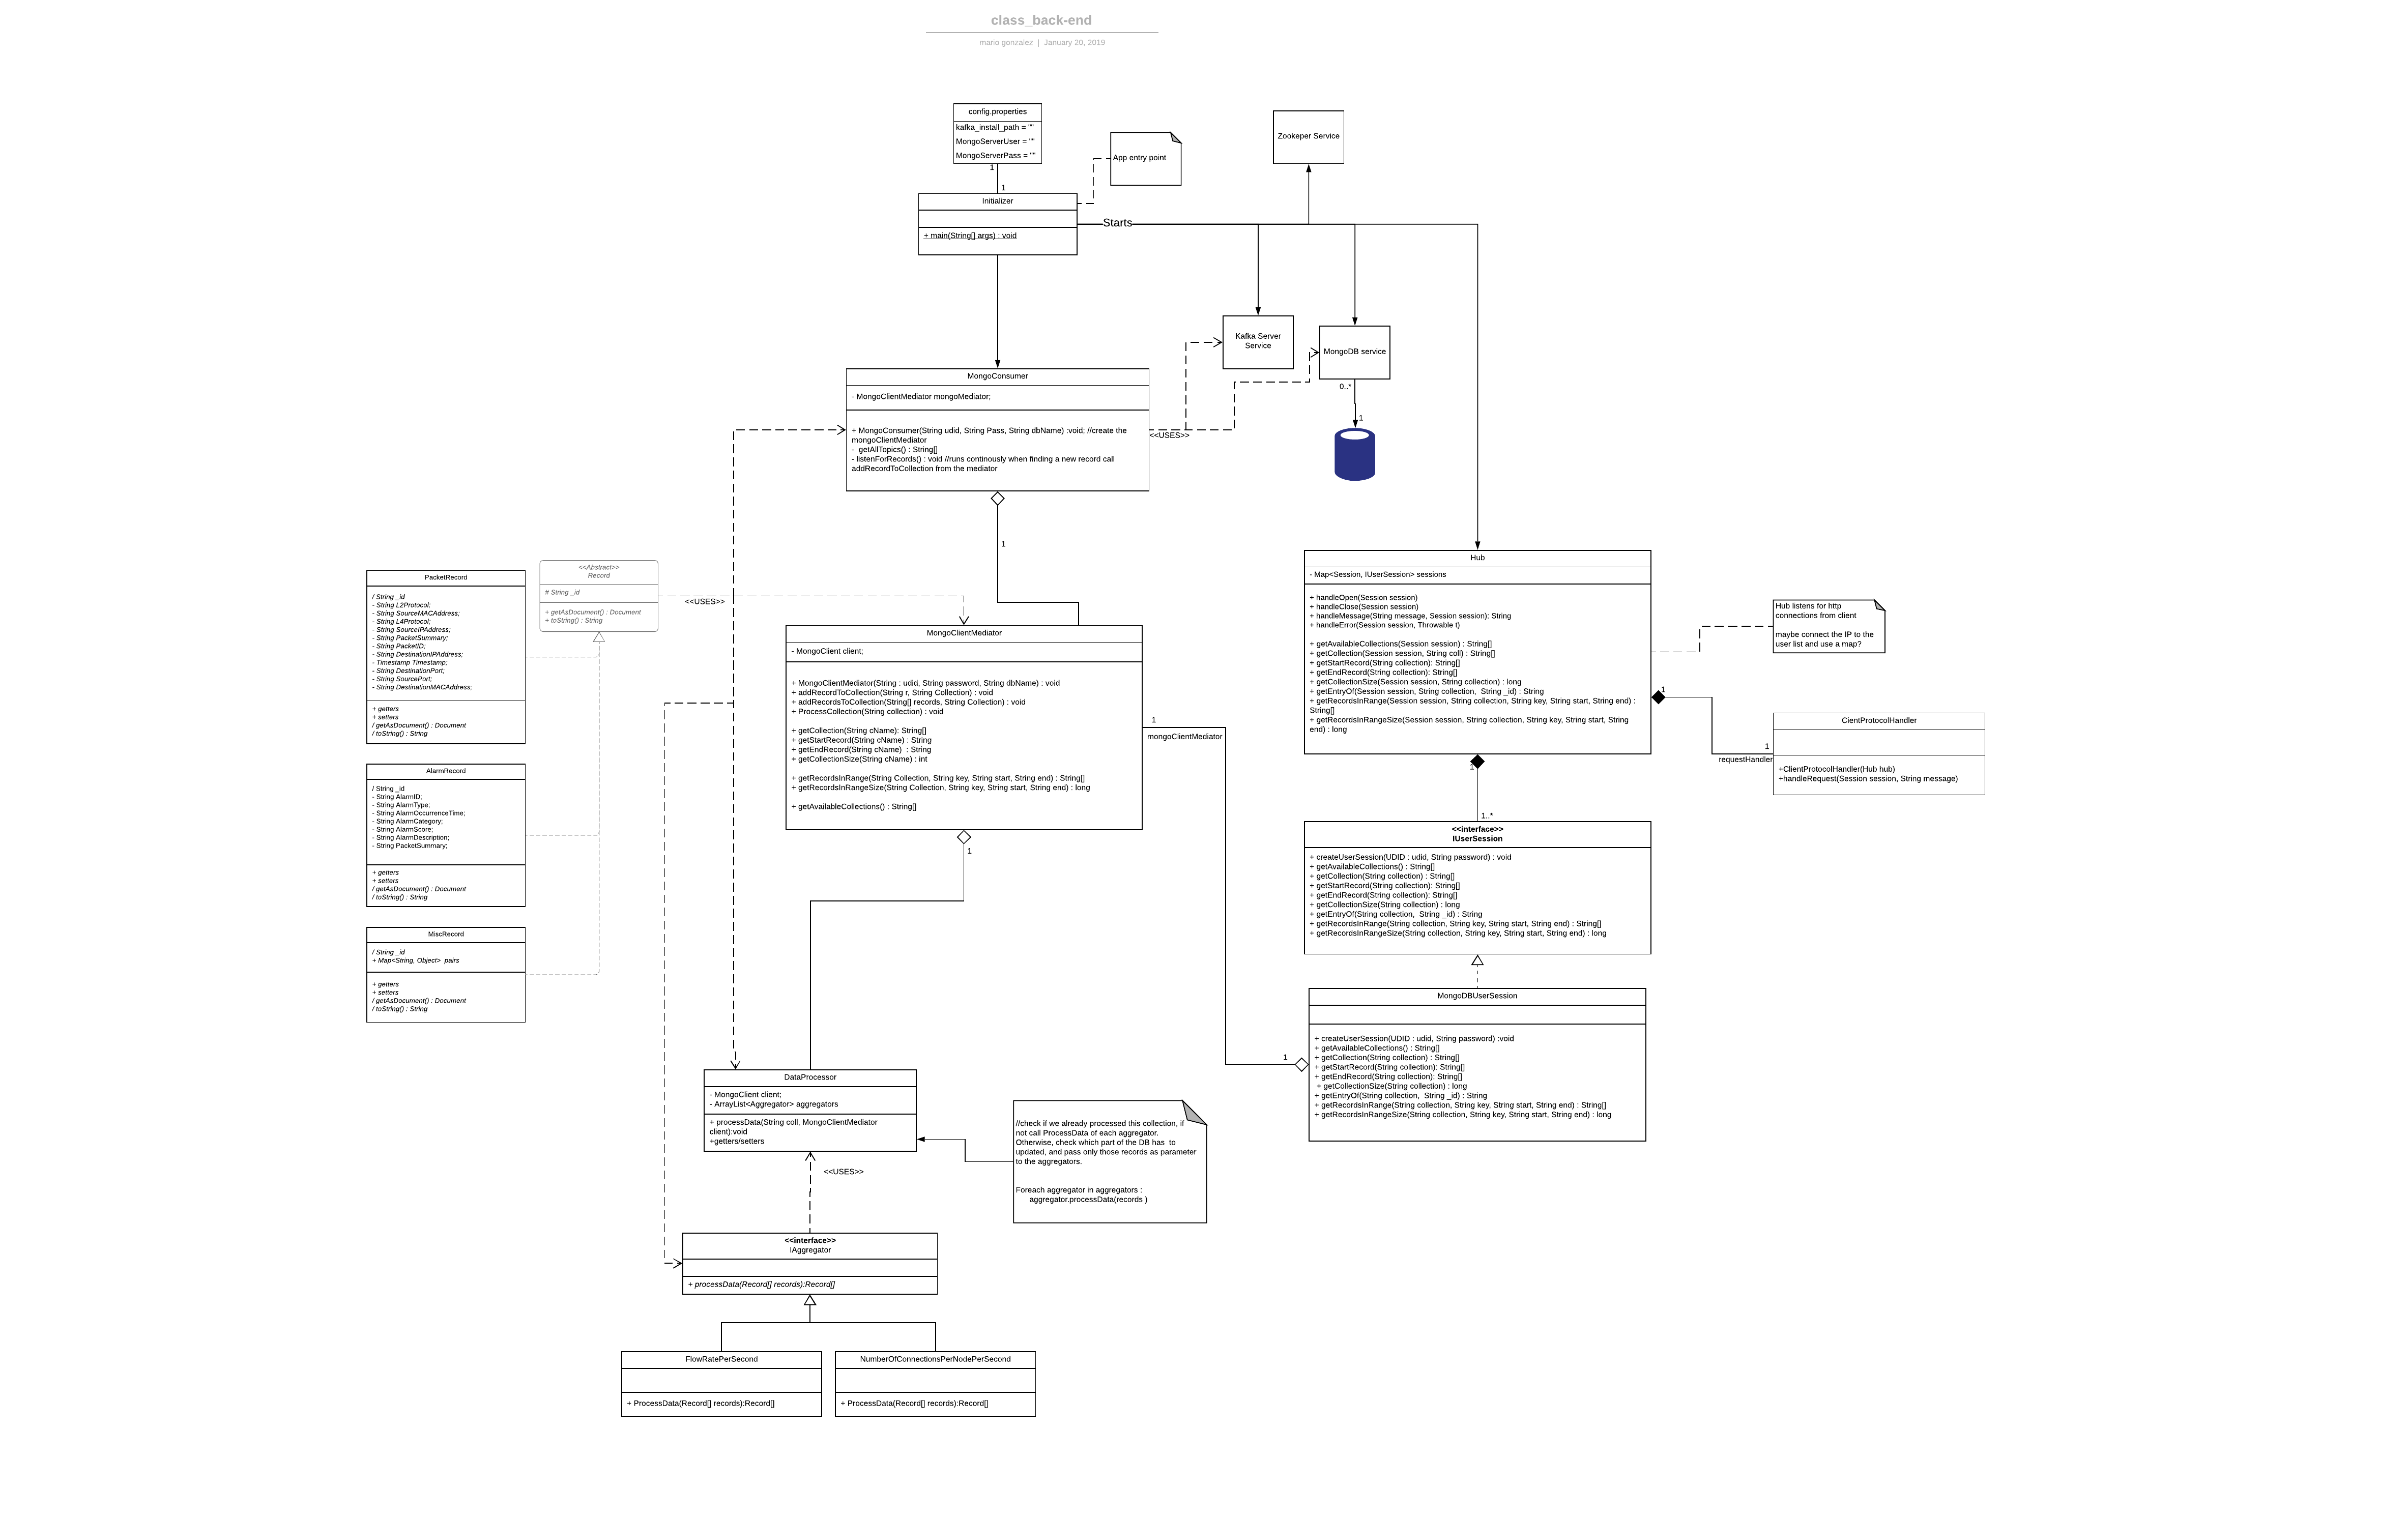
\includegraphics[angle=90,origin=c,max size={\textwidth}{\textheight}]{images_design/class_back-end.png}
	\caption{This is the class diagram for the whole back-end system}
	\label{fig:class_back_end}
\end{figure}
\newpage

\subsection{Sequence Diagrams}
\autoref{fig:seq_server_init}  shows the initalization sequence order, the correspoding class diagram is \autoref{fig:class_back_end_init}, the program dependes on a couple of services namely (in order), the zookeeper serivce, the kafka server service and the mongoDB service. Once all services are up and running the MongoConsumer is created and can start consuming messages and the Hub can start listening to client logins, requests, etc.
\begin{figure}[h!]
	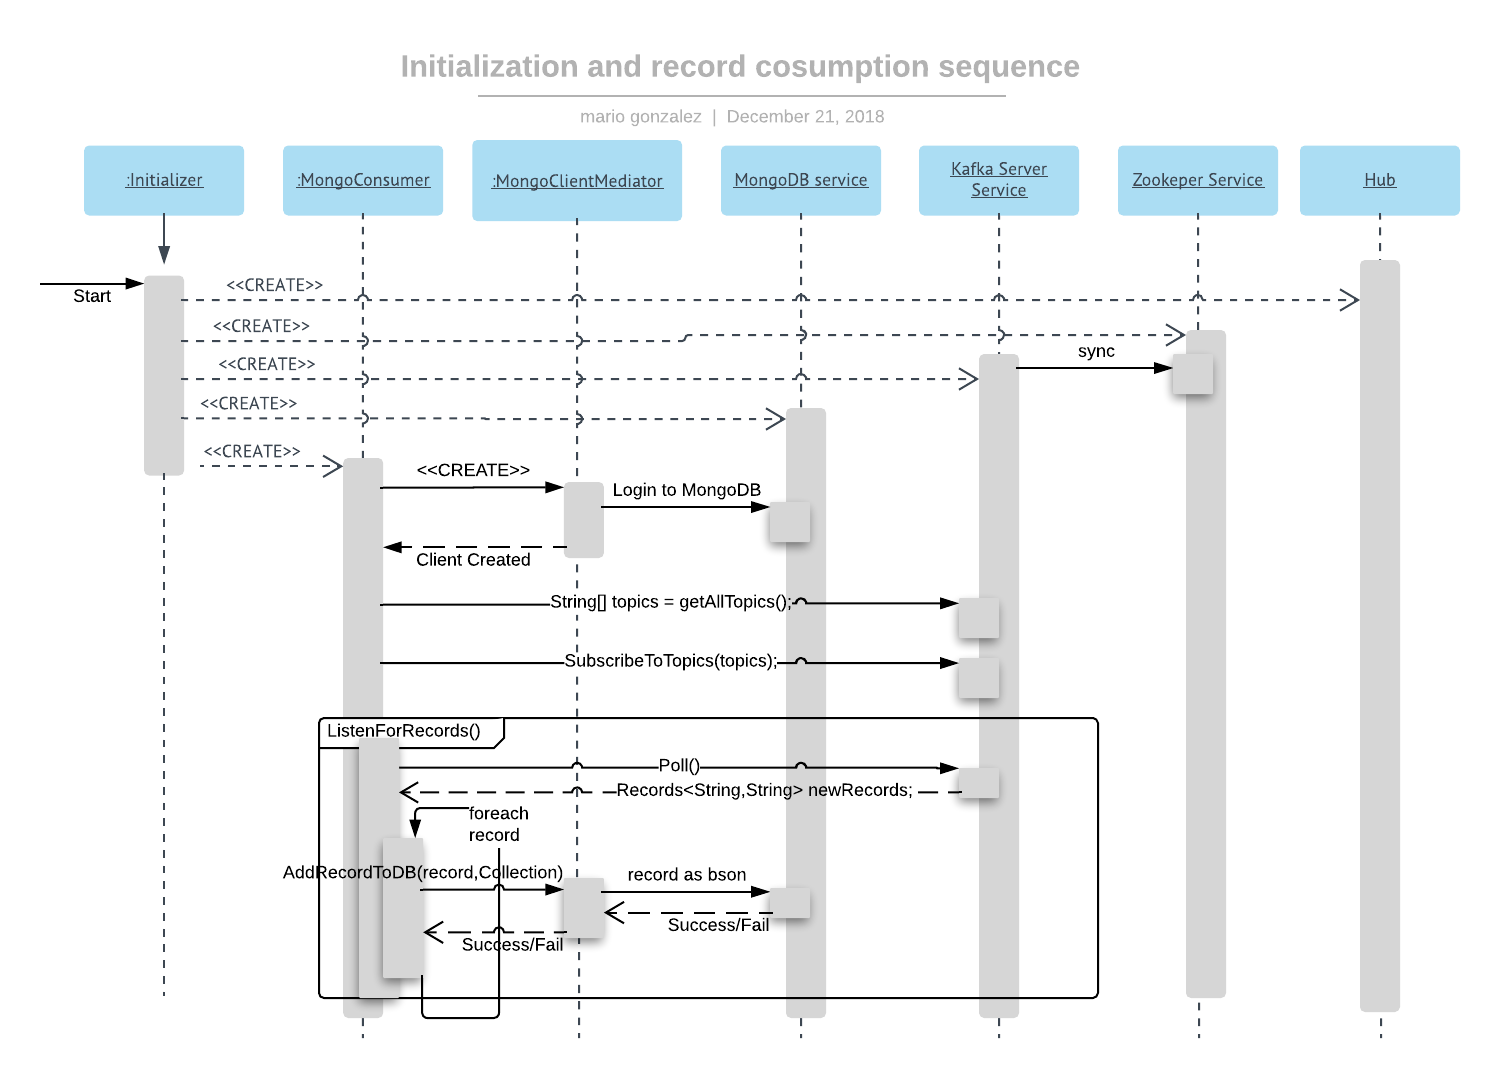
\includegraphics[max size={\textwidth}{\textheight}]{images_design/sequence_server_init.png}
	\caption{Initialization sequence and message consumption}
	\label{fig:seq_server_init}
\end{figure}


\subsection{Activity Diagram}

As previously mentioned for UAC the built-in UAC in MongoDB is used. \\
\autoref{fig:act_UAC} shows the workflow on adding new roles and new user, who upon creation have a role assigned to them, to MongoDB.
\\
A Role determines what can be done and seen within a database. For the purposes of the ADIN INSPECTOR there are three basic roles,
Admin, Operator and Analyst.
The admin role , created by default, can create and destroy users as well as assign specific roles to them. An analyst can see all collections on the database and an Operator can only see part of them.

\begin{figure}[h!]
	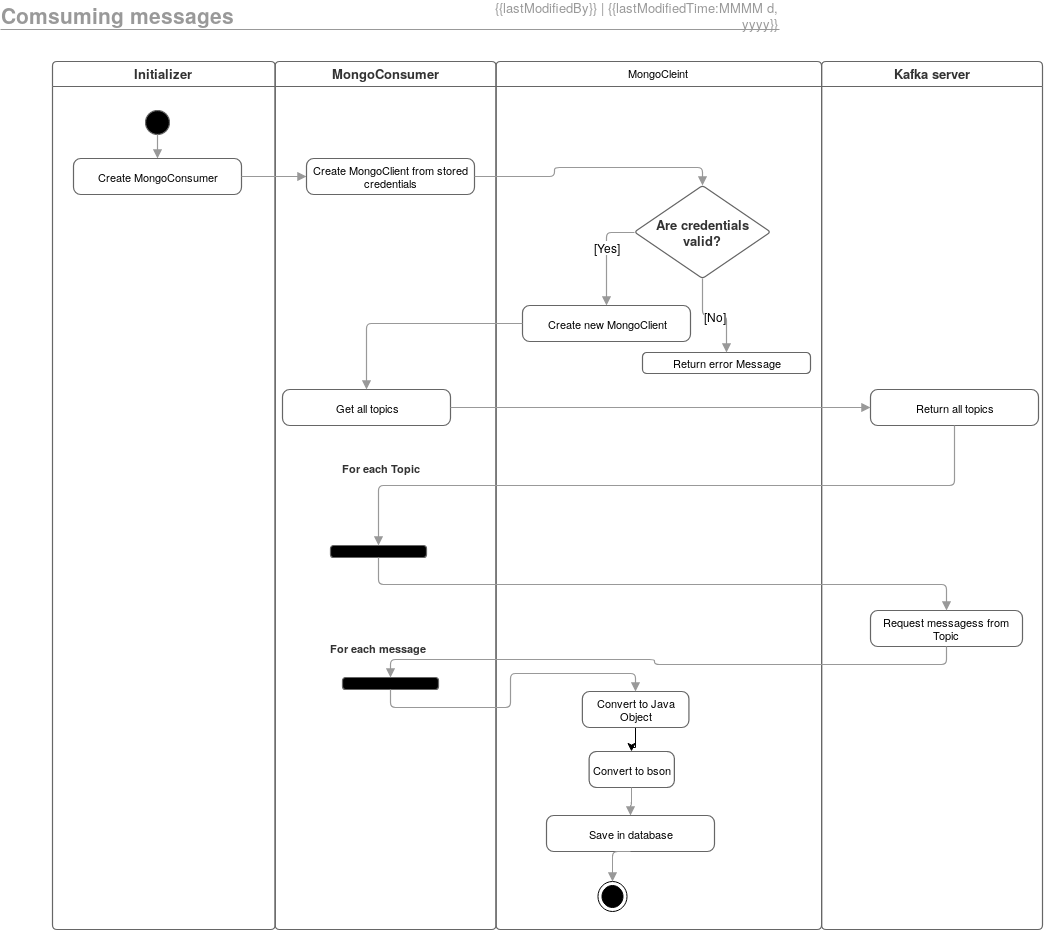
\includegraphics[max size={\textwidth}{\textheight}]{images_design/activity_MongoConsumer.png}
	\caption{Initialization and message consumption workflow.}
	\label{fig:act_consume}
\end{figure}
\clearpage

\begin{figure}[h!]
	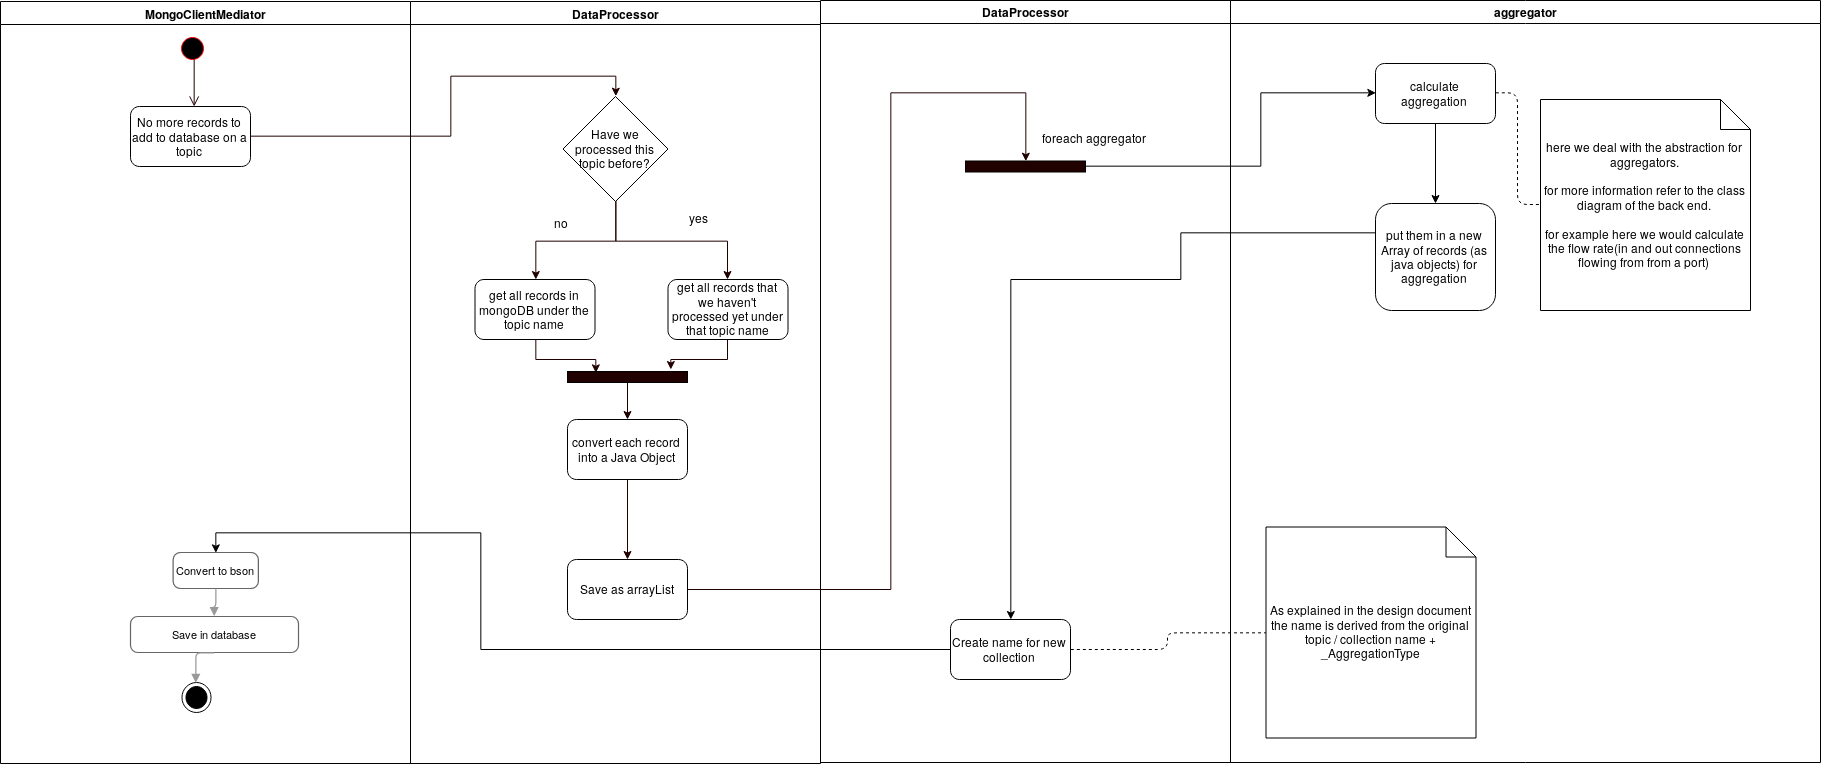
\includegraphics[angle=90,origin=c,max size={\textheight}{\textwidth}]{images_design/activity_ProcessData.png}
	\caption{This diagram shows the processing of Collections and records as well as the addition of extracted data back into the database.}
	\label{fig:act_proc_data}
\end{figure}
\clearpage


\begin{figure}[h!]
	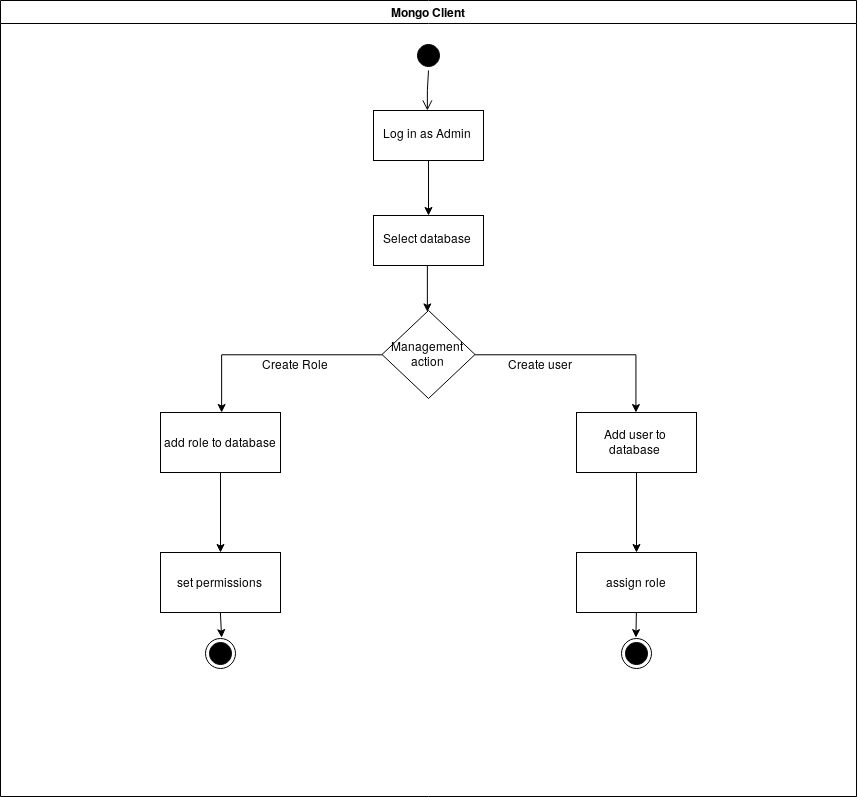
\includegraphics[max size={\textwidth}{\textheight}]{images_design/activity_User-Management.png}
	\caption{User Management workflow}
	\label{fig:act_UAC}
\end{figure}

\clearpage
\section{Changes}
Changes made between version 1.1.0 and version 2.0.0 of this document.

\subsection{Changes to the client-server protocol}
The protocol responses have been made more expressive in general.
\begin{itemize}
	\item{Rename "LOGIN\_TOKEN" request to "AUTH".}
	\item{Rename "LIST\_COL" response to "LIST\_COLL".}
	\item{Expand "session" response with the specifier key "par"}
	\item{Expand "data set" and "collection size" responses with the key "key"}
	\item{Expand "data set" and "collection size" responses with the keys "start" and "end", if they were in the request}
	\item{"data set" and "collection size" responses will now echo back any key-value pairs not specified in the protocol}
	\item{getStartRecord, getEndRecord, and the "single data point" response were added.}
	      item{getEndpoints and the "data endpoints" response were added.}
	      end XXX
\end{itemize}


\chapter{Implementation}\label{sec:implementation}
\section{Introduction}

This implementation report covers changes in the design from the one decribed in the original design phase
and decribes the current state of the implementation by lists of completed and not completed requirements.


\section{Changes in the Design}

Changes are grouped together according to the reason for the change.

\subsection{User Interface changes for better aesthetics and convenience}
\begin{itemize}
  \item{New Login Page
  \\
    Opted for a different graphical design than the one in the mockups due to aesthetic reasons. The functionality and behavior of the login page remains the same as in the design docs.}
    
  \item{Removal of the filter button inside diagram control containers
  \\
  The filters now can be easily accessible inside the config modal of the diagram.}
\end{itemize}

\subsection{User Interface changes for usability improvements}
\begin{itemize}
  \item{New text input box for WebSocket endpoint
  \\
  Added the feature of choosing an arbitrary WebSocket endpoint by persisting the input with Browser Local Storage API, making the frontend application completely standalone and therefore largely simplified the deploy process of the entire DHSTTOS suite.}
  
\end{itemize}

\subsection{Refactoring for cleaner code and changes for convenience reasons}
\begin{itemize}
\item{Data formatting helper function on the frontend
  \\
  Added a helper function \textsf{\textbf{formatData = (\{ groupName, x, y, rawData = [] \}) : Object[] }} which converts the raw data points the frontend receives from the server to structured data arrays which allows easy data passing into the diagram drawing routines.}
  
\item{Add parameter
  \\
	Added parameter DBname to \textsf{\textbf{MongoConsumer(user, pass, dbName)}} for creating a reference to pass onto the MongoClientMediator}

\item{Refactoring
  \\
  Add attribute \textsf{\textbf{private KafkaConsumer<String, String> consumer}} because other functions need to use the consumer}

  \item{Refactor: extract instance attribute}
    \\ 
    Add attribute \textsf{\textbf{private MongoDatabase db}}
    as a reference to the database all methods need to access.

  \item{Convenience functions for different data types}
    \\
    Added variations of \textsf{\textbf{addRecordToCollection(Record record, String collection)}}
    that take a document or an list of documents or an array of record sinstead of a Record.


  \item{Add convenience function}
    \\
    Added \textsf{\textbf{getCollectionAsRecordsArrayList()}}
    to DataProcessor.

  \item{Refactor passing the current mediator object}
  \\
    Add parameter \textsf{\textbf{MongoClientMediator}} to \textsf{\textbf{public static void ProcessData:processData(String collectionName, MongoClientMediator clientMediator)}} so that \textsf{\textbf{processData}} can use it to write the processed data to the database. Remove attribute \textsf{\textbf{ProcessData:MongoClientMediator client}} which was used for this before.


  \item{Add convenience function}
    \\
    Add method \textsf{\textbf{public static void processData(ArrayList<String> collectionNames, MongoClientMediator clientMediator)}} to process a list of collections (instead of calling \textsf{\textbf{processData}} for each collection.
    
  \item{Add convenience function}
    \\
    Added method \textsf{\textbf{public Document getNewAggregatorDocument(Date tstmp)}} for easier handling of date values.

    
  \item{Add convenience attributes}
    \\
    Add the variables Variables
    \textsf{\textbf{private ArrayList<Map<String, Object>> connectionsMapList}} and
    \textsf{\textbf{private Document currentDocument}} to the classes \textsf{\textbf{FlowRatePerSecond}} and \textsf{\textbf{NumberOfConnectionsPerNode}} to
    keep track of which document is being processed now and which connections happened within this second.


\item{Refactoring for cleaner code in protocol handling}
  \\
  Change the protocol parsing in class \textsf{\textbf{ClientProtocoHandler}} from a switch construct to using a private enum.

\end{itemize}

\subsection{Changes due to clarified requirements}
\begin{itemize}
\item{Differing input formats for Date/Timestamp}
  \\
  Split class \textsf{\textbf{PacketRecord}} into \textsf{\textbf{PacketRecordDesFromMongo}} and \textsf{\textbf{PacketRecordDesFromKafka}} to handle different formats.

\end{itemize}


\subsection{Changes due to oversights}

These are changes and additions due to oversights and mistakes in the original design.

\begin{itemize}
  \item{added dbName to MongoClientMediator since we need to know from which DB we want to read/write collections.}
\\

  \item{Unspecified return type}
    \\
    The return type of \textsf{\textbf{public ArrayList<Document> processData( ArrayList<Record> records)}} in \textsf{\textbf{IAggregator}}
was unspecified in the Design document.

  \item{Session handling}
    \\
    To handle session state, \textsf{\textbf{Hub:login()}}, \textsf{\textbf{Hub:loginWithToken()}}, and \textsf{\textbf{Hub:logout()}} were added.
    To keep track of client session state, the private attributes \textsf{\textbf{Hub:sessions}} and \textsf{\textbf{Hub:loginTokens}} were added.

\end{itemize}


\subsection{Changes due to unexpected complexity}
These changes can be attributed to lack of familiarity with the used components and libraries.
\begin{itemize}
  \item{Workaround for Kafka's API}
    \\
    Change \textsf{\textbf{getAllTopics()}} to \textsf{\textbf{getAllTopicsPartitions()}}:
    return a Collection of topic partitions essentially to force kafka to send all records from the start.
    It was complex to make kafka read all the topics from the beginning.
    Secondary aspect: convenient because it relegates topic creation to another method.

  \item{Workaround for Kafka's API}
    \\
    Add method \textsf{\textbf{ArrayList<String> getTopicsForProcessing()}}
  because there are some topics in kakfka which are for internal use, e.g. \_\_consumeroffsets.
 This returns the topics we need to process.
	
  \item{Exception handling}
    \\ 
    The constructor for class \textsf{\textbf{MongoClientMediator}} now throws a LoginFailureException instead of forwarding an unchecked exception.

  \item{Converting between different APIs}
    \\ 
    Add method \textsf{\textbf{mongoIteratorToStringArray(MongoIterable)}}
    because the hub expects an array but the mongodb returns a MongoIterable.

  \item{Making the network protocol more expressive to simplify handling responses}
  \item{Handling the login happening in another websocket session than the main app}
    \\
    \begin{itemize}
    To deal with a restart of the websocket connection when changing from the login page to the main page, session handling was changed. Added the \textsf{\textbf{LOGIN\_TOKEN}} request to the protocol and \textsf{\textbf{Hub:loginWithToken}}.
  Also, the client can add new key-value-pairs to the request which will be returned unchanged by the server.

    \end{itemize}

  \item{Adapt to React and MobX}
    \\
    To adapt to the observer-driven architecture of React and MobX, store data from the server in datastructures \textsf{\textbf{dataStore.rawData}} and \textsf{\textbf{dataStore.alarms}}
    instead of returning it as return values of
    \textsf{\textbf{getAvailableCollections()}},
    \textsf{\textbf{getCollection()}}, \textsf{\textbf{getCollectionSize()}}, \textsf{\textbf{getRecordsInRange()}} and \textsf{\textbf{getRecordsInRangeSize()}} in \textsf{\textbf{wsutils.js}}.

\end{itemize}

\newpage

\section{List of implemented must- and should-requirements}
\subsection{List of implemented must-requirements}
FR100, FR110, FR200, FR300, FR400, FR500, FR700, FR710, FR720, FR1110, FR1300, FR1310
\\
cancelled after Mike left: FR800

\subsection{List of implemented should-requirements}
\begin{itemize}
  \item{FR1332 filter to compute flow rate}
  \begin{itemize}
    \item{this has instead been implemented in the backend which provides this as a new data stream}
  \end{itemize}
  \item{FR1400}
\end{itemize}

\subsection{List of not implemented must-requirements}
\begin{itemize}
  \item{FR600 dynamically change the selected/displayed components}
  \item{FR900 The amount of data can be limited via a slider [...]}
to which all diagrams must update to.
  \item{FR910 Within the slider the user is able to scroll through the timeline and the diagrams need to react in real-time.}
  \item{FR1000 auto scroll}
  \item{FR1100 pick data points, hover}
  \item{FR1200 selecting data points}
  \item{FR1210 create new diagram from selected data}
  \item{FR1330}
\end{itemize}


\subsection{List of not implemented should-requirements}
\begin{itemize}
\item{FR1320 per-diagram filters}
\end{itemize}


\section{Timeline and Delays}
There were delays in the implementation phase caused by
\begin{itemize}
\item{clarification of requirements}
\item{evaluation of graphics libraries}
\item{familiarization with the used APIs and libraries}
\end{itemize}

\begin{figure}[h!]
	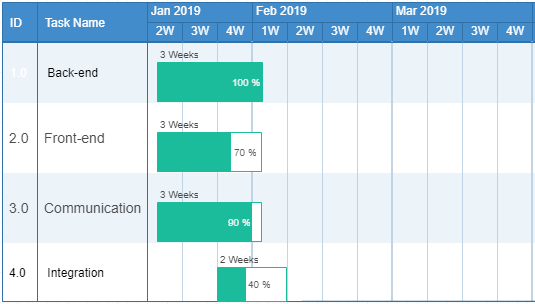
\includegraphics[max size={\textwidth}{\textheight}]{images_implementation/implementation-gantt1.png}
	\caption{The timeline.}
	\label{fig:gantt1}
\end{figure}


\section{Overview of unit tests}
Number of unit tests:\\
\hfill
\\
\begin{tabular}{|p{0.8\textwidth}p{0.1\textwidth}}
DataProcessor & 2\\  Test 1 and 2 both test the functionality of trying to process missing data. In both cases the aggregators responsible should not fail and simply make sure nothing gets added into the Database.\\ \\
Hub & 4\\ Test session handling methods.\\ \\
MockMongoDBUserSession & 4\\ \\
MongoClientMediator & 5 \\ Test1 and 2 and 3: test different credential errors, like missing credentials or credential without access to the necessary databases. All tests cases return a LoginFailureException.\\ 
Test 4 and 5 test handling null reference objects to adding records into MongoDB. In this case then simply, nothing is added into the database.\\ \\
MongoConsumer & 2 \\ Test 1 : tests the case on failure to communicate with kafka, the consumer exists and reports this to the console but operation of all other parts of the program continue since failure of this does not affect working with data already stored in the database.\\
Test2: tests case when the consumer does not have the right credentials to access the MongoDB, the Consumer should then fail to be created and call a LoginFailureException.\\ \\
TestClientProtocolHandler & 2 \\ \\
FormatData. & \\ Testing the GUI would be possible however, this is both complex and time consuming. Due to time constraints minimal testing was done outside of basic functionality.\\ \\
\end{tabular}

\include{chapter_testing}

\end{document}
